\documentclass[krantz1,ChapterTOCs]{krantz} %See documentation for other class options
\usepackage{fixltx2e,fix-cm}
\usepackage{amssymb}
\usepackage{amsmath}
\usepackage{graphicx}
\usepackage{subfigure}
\usepackage{makeidx}
\usepackage{multicol}

%\usepackage[dvips]{hyperref}

\frenchspacing
\tolerance=5000

\makeindex

\newtheorem{theorem}{Theorem}
\newtheorem{exercise}{Exercise}[chapter]
\newtheorem{example}{Example}
\newtheorem{definition}{Definition}
\newtheorem{proof}{Proof}
 %place custom commands and macros here

\begin{document}

\frontmatter

\title{Krantz Template} %This is a placeholder titlepage, it will not be final.
\author{Yours Truly}
\maketitle

\cleardoublepage
\thispagestyle{empty}
\vspace*{\stretch{1}}
\begin{center}
\Large\itshape
To my dog\\
and my cat.
\end{center}
\vspace{\stretch{2}}
\cleardoublepage
\setcounter{page}{7} %previous pages will be reserved for frontmatter to be added in later.
\tableofcontents
\chapter*{Foreword}
I am delighted to introduce the first book on Multimedia Data Mining.  When I came to know about this book project undertaken by two of the most active young researchers in the field, I was pleased that this book is coming in early stage of a field that will need it more than most fields do.  In most emerging research fields, a book can play a significant role in bringing some maturity to the field.  Research fields advance through research papers.  In research papers, however, only a limited perspective could be provided about the field, its application potential, and the techniques required and already developed in the field.  A book gives such a chance.  I liked the idea that there will be a book that will try to unify the field by bringing in disparate topics already available in several papers that are not easy to find and understand.  I was supportive of this book project even before I had seen any material on it.  The project was a brilliant and a bold idea by two active researchers.  Now that I have it on my screen, it appears to be even a better idea.  

Multimedia started gaining recognition in 1990s as a field.  Processing, storage, communication, and capture and display technologies had advanced enough that researchers and technologists started building approaches to combine information in multiple types of signals such as audio, images, video, and  text.  Multimedia computing and communication techniques recognize correlated information in multiple sources as well as insufficiency of information in any individual source.    By properly selecting sources to provide complementary information, such systems aspire, much like human perception system, to create a holistic picture of a situation using only partial information from separate sources.

Data mining is a direct outgrowth of progress in data storage and processing speeds.  When it became possible to store large volume of data and run different statistical computations to explore all possible and even unlikely correlations among data, the field of data mining was born.  Data mining allowed people to hypothesize relationships among data entities and explore support for those.  This field has been put to applications in many diverse domains and keeps getting more applications.  In fact many new fields are direct outgrowth of data mining and it is likely to become a powerful computational tool.\vadjust{\vfill\pagebreak}



\chapter{Preface}
%\addcontentsline{toc}{chapter}{\numberline{}Preface}

\TODO{The preface has not yet been written.  This is just a stub.}

\section*{Audience}
% This book assumes basic understanding of statistical concepts at least at an
% intermediate undergraduate level including regression and analysis of variance
% (for example, at the level of \citet{Neter-etal:90,MendenhallSincich:2003}).
% 
% It is written to appeal to two audiences:
% \begin{itemize*}
%   \item Students and methodologists in the social and health sciences, epidemiology,
%     economics, business
% 	and (bio)statistics
% 	\item Substantive researchers in various disciplines wanting to be able to
% 	apply these methods to their own data
% \end{itemize*}
% 
% It is also assumed that the reader has at least basic knowledge of the \R language and
% environment, including interacting with the \R console (RGui for Windows, R.app for Mac OS X)
% or other graphical user interface (e.g., R Studio), using \R functions in packages,
% getting help for these from \R, etc.  One introductory chapter (\chref{ch:working}) is devoted
% to covering topics beyond such basic skills needed in the book.

\section*{Overview}

\section*{Acknowledgements}


\listoffigures
\listoftables
%%\twocolumn
\chapter*{Contributors}

\begin{multicols}{2}
\contributor{Michael Aftosmis}{NASA Ames Research Center}{Moffett Field, California}

\contributor{Pratul K. Agarwal}{Oak Ridge National Laboratory}{Oak Ridge, Tennessee}

\contributor{Sadaf R. Alam}{Oak Ridge National Laboratory}{Oak Ridge, Tennessee}

\contributor{Gabrielle Allen}{Louisiana State University}{Baton Rouge, Louisiana}

\contributor{Martin Sandve Aln{\ae}s}{Simula Research Laboratory and University of Oslo, Norway}{Norway}

\contributor{Steven F. Ashby} {Lawrence Livermore National Laboratory}{Livermore, California}

\contributor{David A. Bader} {Georgia Institute of Technology}{Atlanta, Georgia}

\contributor{Benjamin Bergen} {Los Alamos National Laboratory}{Los Alamos, New Mexico}

\contributor{Jonathan W. Berry} {Sandia National Laboratories}{Albuquerque, New Mexico}

\contributor{Martin Berzins}{University of Utah}{Salt Lake City, Utah}

\contributor{Abhinav Bhatele}{University of Illinois}{Urbana-Champaign, Illinois}

\contributor{Christian Bischof} {RWTH Aachen University}{Germany}

\contributor{Rupak Biswas} {NASA Ames Research Center}{Moffett Field, California}\vspace*{5pt}

\contributor{Eric Bohm} {University of Illinois}{Urbana-Champaign, Illinois}\vspace*{5pt}

\contributor{James Bordner} {University of California, San Diego}{San Diego, California}\vspace*{5pt}

\contributor{George Bosilca} {University of Tennessee}{Knoxville, Tennessee}\vspace*{5pt}

\contributor{Greg L. Bryan} {Columbia University}{New York, New York}\vspace*{5pt}

\contributor{Marian Bubak} {AGH University of Science and Technology}{
Krak{\'o}w, Poland}\vspace*{5pt}

\contributor{Andrew Canning}{Lawrence Berkeley National
Laboratory}{Berkeley, California}

\contributor{Jonathan Carter} {Lawrence Berkeley National
Laboratory}{Berkeley, California}

\contributor{Zizhong Chen} {Jacksonville State University}{Jacksonville,
Alabama}

\contributor{Joseph R. Crobak} {Rutgers, The State University of New
Jersey}{Piscataway, New Jersey}

\contributor{Roxana E. Diaconescu} {Yahoo! Inc.}{Burbank, California}

\contributor{Peter Diener}
{Louisiana State University}{Baton Rouge, Louisiana}

\contributor{Jack J. Dongarra} {University of Tennessee, Knoxville, 
Oak Ridge National Laboratory, and}{University of Manchester}

\contributor{John B. Drake} {Oak Ridge National Laboratory}{Oak Ridge,
Tennessee}

\contributor{Kelvin K. Droegemeier} {University of Oklahoma}{Norman,
Oklahoma}

\contributor{St{\'e}phane Ethier} {Princeton University}{Princeton, New
Jersey}

\contributor{Christoph Freundl}
{Friedrich--Alexander--Universit{\"a}t}{Erlangen, Germany}

\contributor{Karl F{\"u}rlinger} {University of Tennessee}{Knoxville,
Tennessee}

\contributor{Al Geist} {Oak Ridge National Laboratory}{Oak Ridge,
Tennessee}

\contributor{Michael Gerndt} {Technische Universit{\"a}t
M{\"u}nchen}{Munich, Germany}

\contributor{Tom Goodale}
{Louisiana State University}{Baton Rouge, Louisiana}

\contributor{Tobias Gradl}
{Friedrich--Alexander--Universit{\"a}t}{Erlangen, Germany}

\contributor{William D. Gropp} {Argonne National Laboratory}{Argonne,
Illinois}

\contributor{Robert Harkness} {University of California, San
Diego}{San Diego, California}

\contributor{Albert Hartono} {Ohio State University}{Columbus, Ohio}

\contributor{Thomas C. Henderson} {University of Utah}{Salt Lake City,
Utah}

\contributor{Bruce A. Hendrickson} {Sandia National
Laboratories}{Albuquerque, New Mexico}

\contributor{Alfons G. Hoekstra} {University of Amsterdam}{Amsterdam,
The Netherlands}

\contributor{Philip W. Jones} {Los Alamos National Laboratory}{Los
Alamos, New Mexico}

\contributor{Laxmikant Kal{\'e}} {University of
Illinois}{Urbana-Champaign, Illinois}

\contributor{Shoaib Kamil} {Lawrence Berkeley National
Laboratory}{Berkeley, California}

\contributor{Cetin Kiris} {NASA Ames Research Center}{Moffett Field,
California}

\contributor{Uwe K{\"u}ster} {University of Stuttgart}{Stuttgart,
Germany}

\contributor{Julien Langou} {University of Colorado}{Denver, Colorado}

\contributor{Hans Petter Langtangen}
{Simula Research Laboratory and}{University of Oslo, Norway}

\contributor{Michael Lijewski} {Lawrence Berkeley National
Laboratory}{Berkeley, California}

\contributor{Anders Logg}
{Simula Research Laboratory and}{University of Oslo, Norway}

\contributor{Justin Luitjens} {University of Utah}{Salt Lake City, Utah}

\contributor{Kamesh Madduri} {Georgia Institute of Technology}{Atlanta,
Georgia}

\contributor{Kent-Andre Mardal}
{Simula Research Laboratory and}{University of Oslo, Norway}

\contributor{Satoshi Matsuoka} {Tokyo Institute of Technology}{Tokyo,
Japan}

\contributor{John M. May} {Lawrence Livermore National
Laboratory}{Livermore, California}

\contributor{Celso L. Mendes} {University of Illinois}{Urbana-Champaign,
Illinois}

\contributor{Dieter an Mey} {RWTH Aachen University}{Germany}

\contributor{Tetsu Narumi} {Keio University}{Japan}

\contributor{Michael L. Norman} {University of California, San
Diego}{San Diego, California}

\contributor{Boyana Norris} {Argonne National Laboratory}{Argonne,
Illinois}

\contributor{Yousuke Ohno} {Institute of Physical and Chemical Research
(RIKEN)}{Kanagawa, Japan}

\contributor{Leonid Oliker} {Lawrence Berkeley National
Laboratory}{Berkeley, California}

\contributor{Brian O'Shea} {Los Alamos National Laboratory}{Los Alamos,
New Mexico}

\contributor{Christian D. Ott}
{University of Arizona}{Tucson, Arizona}

\contributor{James C. Phillips} {University of
Illinois}{Urbana-Champaign, Illinois}

\contributor{Simon Portegies Zwart} {University of
Amsterdam,}{Amsterdam, The Netherlands}

\contributor{Thomas Radke}
{Albert-Einstein-Institut}{Golm, Germany}

\contributor{Michael Resch} {University of Stuttgart}{Stuttgart,
Germany}

\contributor{Daniel Reynolds} {University of California, San Diego}{San
Diego, California}

\contributor{Ulrich R{\"u}de}
{Friedrich--Alexander--Universit{\"a}t}{Erlangen, Germany}

\contributor{Samuel Sarholz}
{RWTH Aachen University}{Germany}

\contributor{Erik Schnetter}
{Louisiana State University}{Baton Rouge, Louisiana}

\contributor{Klaus Schulten} {University of Illinois}{Urbana-Champaign,
Illinois}

\contributor{Edward Seidel}
{Louisiana State University}{Baton Rouge, Louisiana}

\contributor{John Shalf} {Lawrence Berkeley National
Laboratory}{Berkeley, California}

\contributor{Bo-Wen Shen} {NASA Goddard Space Flight Center}{Greenbelt,
Maryland}

\contributor{Ola Skavhaug}
{Simula Research Laboratory and}{University of Oslo, Norway}

\contributor{Peter M.A. Sloot} {University of Amsterdam}{Amsterdam, The
Netherlands}

\contributor{Erich Strohmaier} {Lawrence Berkeley National
Laboratory}{Berkeley, California}

\contributor{Makoto Taiji} {Institute of Physical and Chemical Research
(RIKEN)}{Kanagawa, Japan}

\contributor{Christian Terboven}
{RWTH Aachen University,}{Germany}

\contributor{Mariana Vertenstein} {National Center for Atmospheric
Research}{Boulder, Colorado}

\contributor{Rick Wagner} {University of California, San Diego}{San
Diego, California}

\contributor{Daniel Weber} {University of Oklahoma}{Norman, Oklahoma}

\contributor{James B. White, III} {Oak Ridge National Laboratory}{Oak
Ridge, Tennessee}

\contributor{Terry Wilmarth} {University of Illinois}{Urbana-Champaign,
Illinois}

\end{multicols}
\chapter*{Symbols}
\begin{symbollist}{000000}
\symbolentry{$\alpha$}{To solve the generator maintenance scheduling, in the  past, several mathematical techniques have  been applied.}
\symbolentry{$\sigma^2$}{These include integer programming, integer linear programming, dynamic programming, branch and bound etc.}
\symbolentry{$\sum$}{Several heuristic search algorithms have also been developed. In recent years expert systems,}
\symbolentry{$abc$}{fuzzy approaches, simulated annealing and genetic algorithms have also been tested.}
\symbolentry{$\theta\sqrt{abc}$}{This paper presents a survey of the literature}
\symbolentry{$\zeta$}{ over the past fifteen years in the generator}
\symbolentry{$\partial$}{maintenance scheduling. The objective is to}
\symbolentry{sdf}{present a clear picture of the available recent literature}
\symbolentry{ewq}{of the problem, the constraints and the other aspects of}
\symbolentry{bvcn}{the generator maintenance schedule.}
\end{symbollist}

\mainmatter

\part{This is What a Part Would Look Like}
\chapter{Basic Concepts}

A component part for an electronic item is
manufactured at one of three different factories, and then delivered to
the main assembly line.Of the total number supplied, factory A supplies
50\%, factory B 30\%, and factory C 20\%. Of the components
manufactured at factory A, 1\% are faulty and the corresponding
proportions for factories B and C are 4\% and 2\% respectively. A
component is picked at random from the assembly line. What is the
probability that it is faulty? 

\section{Introduction}\label{intro}
The term reliability usually refers to the probability that a
component or system will operate satisfactorily either at any particular
instant at which it is required or for a certain length of
time. Fundamental to quantifying reliability s a knowledge of how to
define, assess and combine probabilities \cite{Bontempi2005Adaptive}. This may hinge on identifying the
form of the variability which is nherent n most processes. If all
components had a fixed known lifetime there would be no need to model
reliability.

\begin{enumerate}[1.]
\item A component part for an electronic item is
manufactured at one of three different factories.

\item A component part $x$ for an electronic item is
manufactured at one of three different factories.
\begin{enumerate}
\item A component part for an electronic item is
manufactured at one of three different factories.

\item A component part $x$ for an electronic item is
manufactured at one of three different factories.
\begin{enumerate}[iv.]
\item A component part for an electronic item is
manufactured at one of three different factories.

\item A component part $x$ for an electronic item is
manufactured at one of three different factories.

\item A component part for an electronic item is
manufactured at one of three different factories.

\item A component part 1, 2, 3, 4 for an electronic item is
manufactured at one of three different factories.

\item A component part for enumerate list of an electronic item is
manufactured at one of three different factories.

\end{enumerate}

\item A component part for an electronic item is
manufactured at one of three different factories.

\item A component part 1, 2, 3, 4 for an electronic item is
manufactured at one of three different factories.

\item A component part for enumerate list of an electronic item is
manufactured at one of three different factories.

\end{enumerate}

\item A component part for an electronic item is
manufactured at one of three different factories.

\item A component part 1, 2, 3, 4 for an electronic item is
manufactured at one of three different factories.

\item A component part for enumerate list of an electronic item is
manufactured at one of three different factories.

\end{enumerate}

\subsection{A component part}
A component part for an electronic item is
manufactured at one of three different factories, and then delivered to
the main assembly line.Of the total number supplied, factory A supplies
50\%, factory B 30\%, and factory C 20\%. Of the components
manufactured at factory A, 1\% are faulty and the corresponding
proportions for factories B and C are 4\% and 2\% respectively. A
component is picked at random from the assembly line. What is the
probability that it is faulty \cite{ilyas2004hsn}? 
A component part for an electronic item is
manufactured at one of three different factories, and then delivered to
the main assembly line. Of the total number supplied, factory A supplies
50\%, factory B 30\%, and factory C 20\%. Of the components
manufactured at factory A, 1\% are faulty and the corresponding
proportions for factories B and C are 4\% and 2\% respectively. A
component is picked at random from the assembly line. What is the
probability that it is faulty? 
A component part for an electronic item is
manufactured at one of three different factories, and then delivered to
the main assembly line.Of the total number supplied, factory A supplies
50\%, factory B 30\%, and factory C 20\%. Of the components
manufactured at factory A, 1\% are faulty and the corresponding
proportions for factories B and C are 4\% and 2\% respectively. A
component is picked at random from the assembly line. What is the
probability that it is faulty? 

\begin{VF}
``A Process is a structured, measured set of activities designed to produce a specific output for a particular customer
or market---A process is thus a specific ordering of work activities across time and space, with a beginning, an end.
and clearly defined inputs and outputs: a structure for action.''

\VA{Thomas Davenport}{Senior Adjutant to the Junior Marketing VP}
\end{VF}


\begin{table}%1
%\noautomaticrules
\tabletitle{Now we are engaged $(a_g^a)$ $\big(a_g^a\big)$ in a great civil war, testing whether that
nation, or any nation so conceived.}%
\begin{tabular}{lccc}
\tch{Scene}    &\tch{Reg. fts.} &\tch{Hor. fts.} &\tch{Ver. fts.}\\
Ball &19, 221 &4, 598   &3, 200\\
Pepsi$^a$&46, 281 &6, 898 &5, 400\\
Keybrd$^b$   &27, 290 &2, 968 &3, 405\\
Pepsi    &14, 796 &9, 188 &3, 209\\
\end{tabular}
\end{table}

\textbf{MultiRelational $k$-Anonymity.} Most works on $k$-anonymity focus on anonymizing a single data table; however, a real-life \cite{diamantaras1996pcn} database usually contains multiple relational tables. This has proposed a privacy model called \emph{MultiR $k$-anonymity} to ensure $k$-anonymity on multiple relational tables. Their model assumes that a relational database contains a person-specific table $PT$ and a set of tables $T_1,\cdots,T_n$, where $PT$ contains a person identifier $Pid$ and some sensitive attributes, and $T_i$, for $1 \leq i \leq n$, contains some foreign keys, some attributes in $QID$, and sensitive attributes. The general privacy notion is to ensure that for each record owner $o$ contained in the join of all tables $PT \Join T_1 \Join \cdots \Join T_n$, there exists at least $k-1$ other record owners share the same $QID$ with $o$. It is important to emphasize that the $k$-anonymization is applied at the \emph{record owner} level, not at the \emph{record} level in traditional $k$-anonymity. This idea is similar to $(X,Y)$-anonymity, where $X=QID$ and $Y=\{Pid\}$.

Most works on $k$-anonymity focus on anonymizing a single data table; however, a real-life \cite{diamantaras1996pcn} database usually contains multiple relational tables. This has proposed a privacy model called \emph{MultiR $k$-anonymity} to ensure $k$-anonymity on multiple relational tables. Their model assumes that a relational database contains a person-specific table $PT$ and a set of tables $T_1,\cdots,T_n$, where $PT$ contains a person identifier $Pid$ and some sensitive attributes, and $T_i$, for $1 \leq i \leq n$, contains some foreign keys, some attributes in $QID$, and sensitive attributes. The general privacy notion is to ensure that for each record owner $o$ contained in the join of all tables $PT \Join T_1 \Join \cdots \Join T_n$, there exists at least $k-1$ other record owners share the same $QID$ with $o$. It is important to emphasize that the $k$-anonymization is applied at the \emph{record owner} level, not at the \emph{record} level in traditional $k$-anonymity. This idea is similar to $(X,Y)$-anonymity, where $X=QID$ and $Y=\{Pid\}$.

\begin{table}[b!]%2
\tabletitle[Short Table Caption]{Now we are engaged $(a_g^a)$ $\big(a_g^a\big)$ in a great civil war, testing whether that
nation, or any nation so conceived.}%}{%
\begin{tabular}{lccc}
\tch{Scene}    &\tch{Reg. fts.} &\tch{Hor. fts.} &\tch{Ver. fts.}\\
\multicolumn{4}{@{}l@{}}{\tsh{Table Head}}\\[3pt]\hline\\[-6pt]
Ball &19, 221 &4, 598   &3, 200\\
Pepsi &46, 281 &6, 898 &5, 400\\
Keybrd   &27, 290 &2, 968 &3, 405\\
Pepsi    &14, 796 &9, 188 &3, 209\\
\end{tabular}
\end{table}

\begin{shadebox}
A component part for an electronic item is
manufactured at one of three different factories, and then delivered to
the main assembly line.Of the total number supplied, factory A supplies
50\%, factory B 30\%, and factory C 20\%. Of the components
manufactured at factory A, 1\% are faulty and the corresponding
proportions for factories B and C are 4\% and 2\% respectively. A
component is picked at random from the assembly line. What is the
probability that it is faulty? 
\end{shadebox}

In most literature on PPDP, they \cite{jolliffe2002pca} consider a more relaxed, yet more practical, notion of privacy protection by assuming limited attacker's background knowledge. Below, the term ``victim" refers to the record owner being linked. We can broadly classify linking models to two families.

\begin{extract}
A component part for an electronic item is \cite{hyvarinen2001ica}
manufactured at one of three different factories, and then delivered to
the main assembly line.Of the total number supplied, factory A supplies
50\%, factory B 30\%, and factory C 20\%. Of the components
manufactured at factory A, 1\% are faulty and the corresponding
proportions for factories B and C are 4\% and 2\% respectively. 
\end{extract}


One family considers a privacy threat occurs when an attacker is able to link a record owner to a record in a published data table, to a sensitive attribute in a published data table, or to the published data table itself. We call them \emph{record linkage}, \emph{attribute linkage}, and \emph{table linkage}, respectively. In all types of linkages, we assume that the attacker knows the $QID$ of the victim. In record and attribute linkages, we further assume that the attacker knows the presence of the victim's record in the released table, and seeks to identify the victim's record and/or sensitive information from the table \cite{yao2002can}. In table linkage, the attack seeks to determine the present or absent of the victim's record in the released table. A data table is considered to privacy preserved if the table can effectively prevent the attacker from successfully performing these types of linkages on the table \cite{madden2002tta}. Sections~\ref{intro}-\ref{sec:reclinkage} study this family of privacy models.
\begin{equation}
\mbox{var}\widehat{\Delta} = \sum_{j = 1}^t \sum_{k = j+1}^t
\mbox{var}\,(\hat{\alpha}_j - \hat{\alpha}_k)  = \sum_{j = 1}^t
\sum_{k = j+1}^t \sigma^2(1/n_j + 1/n_k). \label{2delvart2}
\end{equation}


An obvious measure of imbalance is just the difference in the
number of times the two treatments are allocated
\begin{equation}
D_n = \mathcal{M}|n_A - n_B|. \label{2deffD}
\end{equation}
For rules such as deterministic allocation, for which the expected
value of this difference can be calculated, we obtain the population
value ${\cal D}_n$.

\begin{shortbox}
\Boxhead{Box Title Here}
Another family aims at achieving the \emph{uninformative principle}: The published table should provide the attacker with little additional information beyond the background knowledge. There should not be a large difference between the prior and posterior beliefs; otherwise, there is a privacy threat~\cite{jain2004ass, jolliffe2002pca}. Many privacy models in this family are designed for statistical database and do not distinguish attributes in $T$ into $QID$, but some of them could also thwart record, attribute, and table linkages. Section~\ref{intro} studies this family of privacy models.

Let $m$ be a prime number. With the addition and multiplication as 
defined above, $Z_m$ is a field.
\end{shortbox}

\begin{theorem}\label{1th:Z_m}
Let $m$ be a prime number. With the addition and multiplication as 
defined above, $Z_m$ is a field.
\end{theorem}

\begin{proof}
Most of the proof of this theorem is routine.  It is clear that $0\in Z_m$ 
and $1\in Z_m$ are the 
zero element and identity element. If $a\in Z_m$ and $a\ne 0$, then $m-a$ 
is the additive inverse of $a$. If $a\in Z_m$ and $a\ne 0$, then the 
greatest common divisor of $a$ and $m$ is 1, and hence
there exist integers $s$ and $t$ such that $sa+tm=1$. Thus $sa=1 -tm$ is 
congruent to 1 modulo $m$. Let $s^*$ be the integer in $Z_m$ 
congruent to $s$ 
modulo $m$. Then we also have $s^*a\equiv 1\  \mbox{mod}\ m$. Hence $s^*$ 
is 
the multiplicative inverse of $a$ modulo $m$. Verification of the rest of 
the field properties is now routine.\end{proof}



\section{Record Linkage Model}\label{sec:reclinkage}

In the privacy attack of \emph{record linkage}, some value $qid$ on $QID$ identifies a small number of records in the released table $T$,
called a \emph{group}. If the victim's $QID$ matches the value
$qid$, the victim is vulnerable to being linked to the small
number of records in the group \cite{madden2005taq}. In this case, the attacker faces
only a small number of possibilities for the victim's record, and
with the help of additional knowledge, there is a chance that the
attacker could uniquely identify the victim's record from the
group.


%%%\begin{table}
%%%    \tabletitle{Examples for illustrating attacks}
%%%    \begin{tabular}{|c|c|c|c|}
%%%        \hline
%%%        \textbf{Job} & \textbf{Sex} & \textbf{Age} & \textbf{Disease} \\
%%%        \hline
%%%        Engineer & Male & 35 & Hepatitis \\
%%%        Engineer & Male & 38 & Hepatitis \\
%%%        Lawyer & Male & 38 & HIV \\
%%%        Writer & Female & 30 & Flu \\
%%%        Writer & Female & 30 & HIV \\
%%%        Dancer & Female & 30 & HIV \\
%%%        Dancer & Female & 30 & HIV \\
%%%        \hline
%%%    \end{tabular}
%%%    \label{table:rawpatient}
%%%\end{table}



\subsection{A component part}
A component part for an electronic item is
manufactured at one of three different factories, and then delivered to
the main assembly line.Of the total number supplied, factory A supplies
50\%, factory B 30\%, and factory C 20\%. Of the components
manufactured at factory A, 1\% are faulty and the corresponding
proportions for factories B and C are 4\% and 2\% respectively. A
component is picked at random from the assembly line. What is the
probability that it is faulty? 



\begin{figure}

\includegraphics[width=350pt, height=200pt]{Chapters/chapter1/figures/cat.eps}
%%\centerline{\epsfig{/Chapters/chapter1/figures/cat.eps,width=.8\textheight,height=.4\textwidth}}
\caption[List of figure caption goes here]{Figure caption goes here.}
\end{figure}



\begin{figure}[htb]

\includegraphics[width=200pt, height=200pt]{Chapters/chapter1/figures/cat.eps}
%%\centerline{\epsfig{figure=cat.eps,width=.5\textheight,height=.4\textwidth}}
\caption[Short figure caption]{Figure caption goes here. Figure caption goes here.
Figure caption goes here. Figure caption goes here. Figure caption goes here.
Figure caption goes here.}
\end{figure}





\begin{figure}
\begin{center}
\subfigure[\label{f8a}]{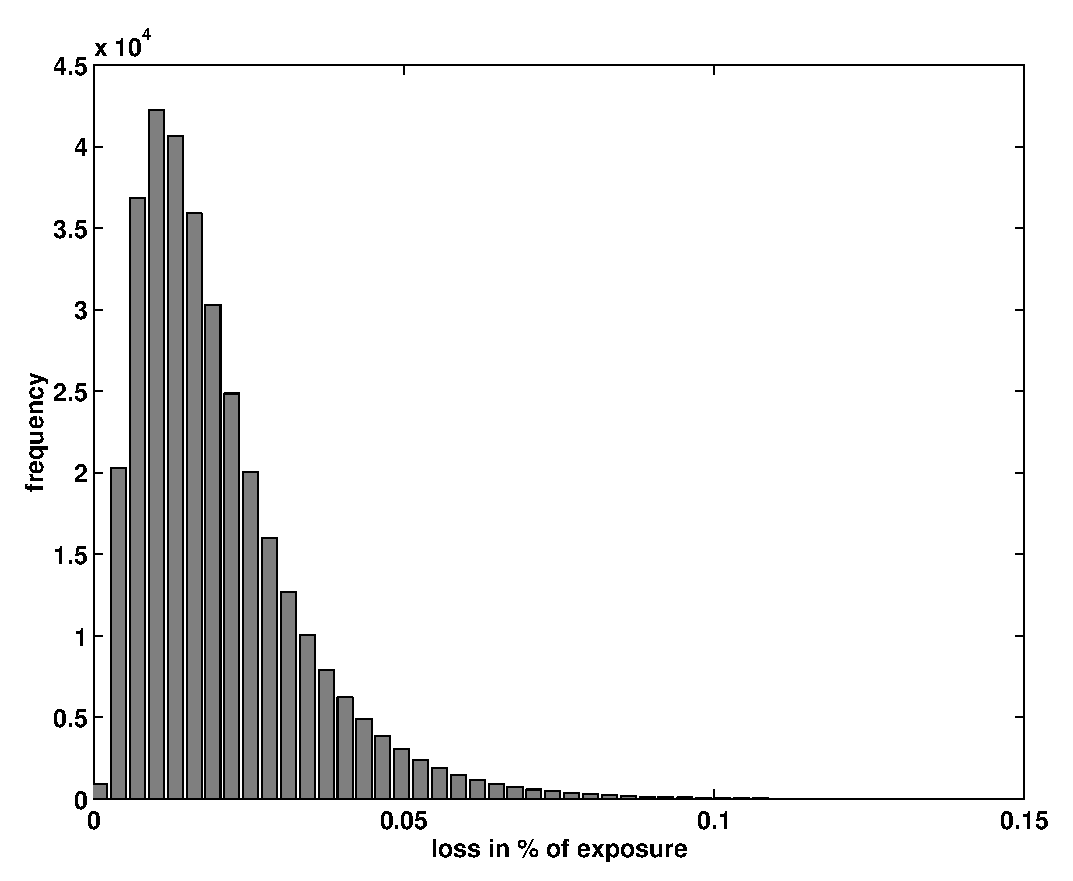
\includegraphics[angle=90,width=7cm,height=7cm,angle=-90]{Chapters/chapter1/figures/Histogram.eps}}
\subfigure[\label{f8b}]{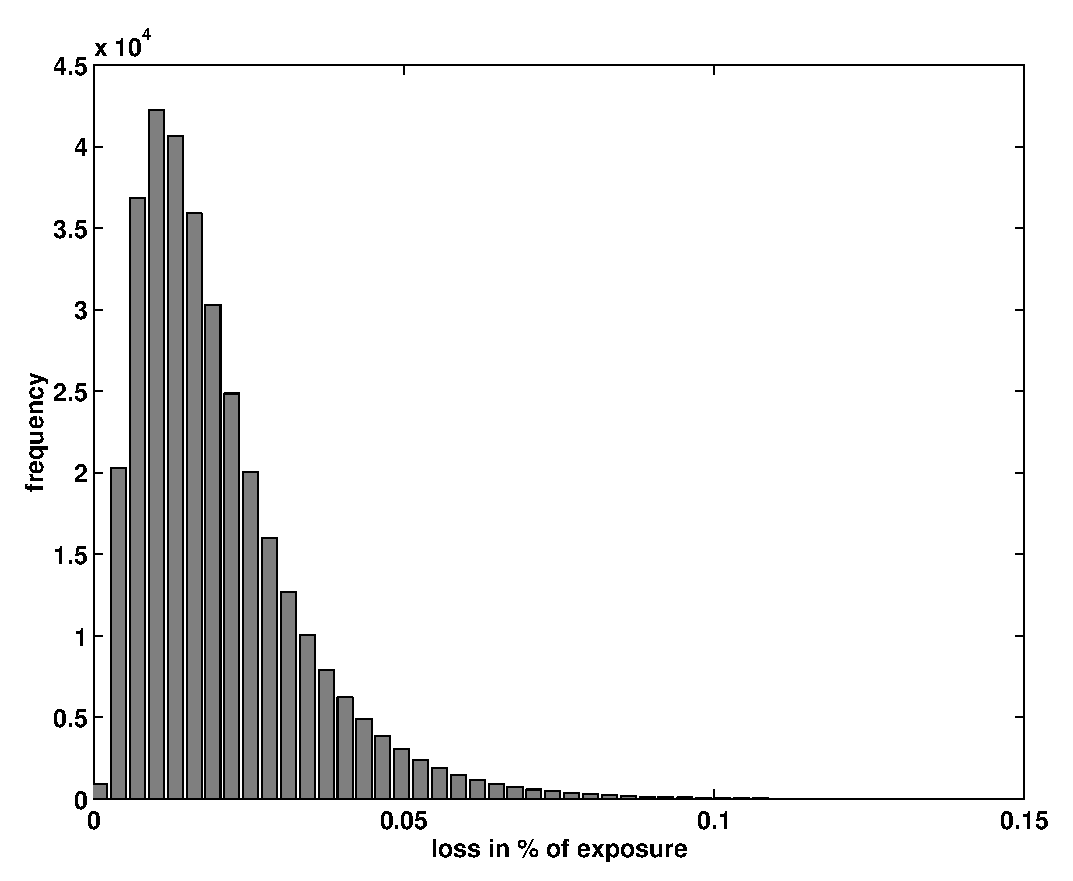
\includegraphics[angle=90,width=7cm,height=7cm,angle=-90]{Chapters/chapter1/figures/Histogram.eps}}
\end{center}
\caption[The bar charts depict the different risk contributions]{The bar charts depict the different risk contributions (top: 99\% quantile, bottom: 99.9\% quantile) of the business areas of a bank. The black bars
are based on a Var/Covar approach, the white ones correspond to shortfall risk.}
\end{figure}

\subsubsection{H3 A component part }
A component part for an electronic item is
manufactured at one of three \cite{mardia1979ma} different factories, and then delivered to
the main assembly line.Of the total number supplied, factory A supplies
50\%, factory B 30\%, and factory C 20\%. Of the components
manufactured at factory A, 1\% are faulty and the corresponding
proportions for factories B and C are 4\% and 2\% respectively. A
component is picked at random from the assembly line. What is the
probability that it is faulty? 


A fundamental notion \cite{yao2002can} is that of a\index{subspace}\index{vector 
space!subspace of} subspace of $F^n$. Let $V$ be a nonempty subset of 
$F^n$. Then $V$ is a {\it subspace} of $F^n$ provided $V$ is closed 
under vector addition and scalar multiplication, that is, 
\begin{enumerate} 
\item[\rm (a)] For all $u$ and $v$ in $V$, $u+v$ is 
also in $V$. 
\item[\rm (b)] For all $u$ in $V$ and $c$ in $F$, $cu$ is 
in $V$. 
\end{enumerate} 
Let $u$ be in the subspace $V$. Because $0u=0$, 
it follows that the zero vector is in $V$. Similarly, $-u$ is in $V$ 
for all $u$ in $V$. A simple example of a subspace of $F^n$ is the set 
of all vectors $(0,a_2,\ldots,a_n)$ with first coordinate equal to 0. 
The zero vector itself is a subspace.

\begin{definition}\label{1def:linearcomb}{\rm
Let $u^{(1)},u^{(2)},\ldots,u^{(m)}$ be vectors in $F^n$, and let 
$c_1,c_2,\ldots,c_m$ be scalars. Then the vector
\[c_1u^{(1)}+c_2u^{(2)}+\cdots+c_mu^{(m)}\]
is called a {\it linear combination} \index{linear combination} of $u^{(1)},u^{(2)},\ldots,u^{(m)}$.
If $V$ is a subspace of $F^n$, then $V$ is closed under vector addition and 
scalar multiplication, and it follows easily by induction that a 
linear combination of vectors in $V$ is also a vector in $V$. Thus 
{\it subspaces 
are closed under linear combinations}; in fact, this can be taken as the 
defining property of subspaces.
The vectors $u^{(1)},u^{(2)},\ldots,u^{(m)}$ {\it span} $V$ \index{spanning set}
(equivalently, form a {\it spanning set} of $V$) provided every vector in 
$V$ 
is a linear combination of $u^{(1)},u^{(2)},\ldots,u^{(m)}$. The zero 
vector can be written as a linear combination of 
$u^{(1)},u^{(2)},\ldots,u^{(m)}$ with all scalars equal to 0; this is a 
{\it trivial linear combination}.\index{linear combination!trivial} The vectors
$u^{(1)},u^{(2)},\ldots,u^{(m)}$ are {\it linearly dependent} provided 
there are scalars $c_1,c_2,\ldots,c_m$, not all of which are zero, such 
that
\[c_1u^{(1)}+c_2u^{(2)}+\cdots+c_mu^{(m)}=0,\]
that is, the zero vector can be written as a {\it nontrivial linear \index{linear combination!nontrivial} 
combination} of $u^{(1)},u^{(2)},\ldots,u^{(m)}$.
For example, the vectors $(1,4), (3,-1)$, and $(3,5)$ in $\Re^2$ are 
linearly 
dependent since
\[3(1,4)+1(3,-2)-2(3,5)=(0,0).\] Vectors are {\it linearly independent} provided  they are not linearly dependent.\index{linearly independent}
The vectors 
$u^{(1)},u^{(2)},\ldots,u^{(m)}$ are a {\it basis} \index{basis} of $V$ provided they are  
linearly independent and span $V$.
By an {\it ordered basis} \index{basis!ordered} we mean a basis in which the vectors of the basis are listed 
in a specified order; to indicate that we have an ordered basis we write
$(u^{(1)},u^{(2)},\ldots,u^{(m)})$. 
A spanning set $S$ of $V$ is a \index{spanning set!minimal} {\it minimal spanning set of $V$} provided that
each set 
of vectors obtained from $S$ by removing a vector is not a spanning set 
for $V$.
A linearly independent set $S$ of vectors of $V$ is a {\it maximal linearly \index{linearly independent!maximal}
independent set of vectors of $V$} provided that for each vector $w$ of 
$V$ that 
is not in $S$, $S\cup\{w\}$ is  linearly dependent (when this happens, 
$w$ must be  a linear combination of the vectors in 
$S$).\hfill{$\Box$}
}\end{definition}

In addition to matrix addition, subtraction, and multiplication, there is 
one additional operation that we define now. It's perhaps the simplest of 
them all. Let $A=[a_{ij}]$ be an $m$ by $n$ matrix and let $c$ be a 
number \cite{hyvarinen2001ica}. Then the matrix $c\cdot A$, or simply $cA$, is the $m$ by $n$ 
matrix obtained by multiplying each entry of $A$ by $c$:
\[c A=[ca_{ij}].\]\index{matrix!scalar multiplication} \index{matrix!scalar multiple of}
The matrix $c A$ is called a {\it scalar multiple} of $A$.

\begin{VT1}

\VH{Think About It...}

Commonly thought of as the first modern computer, ENTAC was built in 1944. It took up more space than an 18-wheeler's
tractor trailer and weighed more than 17 Chevrolet Camaros. It consumed 140,000 watts of electricity while executing
up to 5,000 basic arithmetic operations per second. One of today's popular microprocessors, the 486, is built on a
tiny piece of silicon about the size of a dime.

\VT
With the continual expansion of capabilities, computing power will eventually exceed the capacity for human
comprehension or human control.

\VTA{The Information Revolution}{Business Week}
\end{VT1}


\section{Glossary}
\begin{Glossary}
\item[360 Degree Review] Performance review that includes feedback from superiors, peers, subordinates, and clients.
\item[Abnormal Variation] Changes in process performance that cannot be accounted for by typical day-to-day variation. Also referred to as
non-random variation.
\item[Acceptable Quality Level (AQL)] The minimum number of parts that must comply with quality standards, usually stated as a percentage.
\item[Activity] The tasks performed to change inputs into outputs.
\item[Adaptable] An adaptable process is designed to maintain effectiveness and efficiency as requirements change. The process is
deemed adaptable when there is agreement among suppliers, owners, and customers that the process will meet
requirements throughout the strategic period.
\end{Glossary}




%\chapter{Fitting and graphing discrete distributions}\label{ch:discrete}
\begin{center}
 \rule[-4pt]{0.5pt}{4pt}\hrulefill\rule[-4pt]{0.5pt}{4pt}\\
 \begin{minipage}[c]{.33\linewidth}
  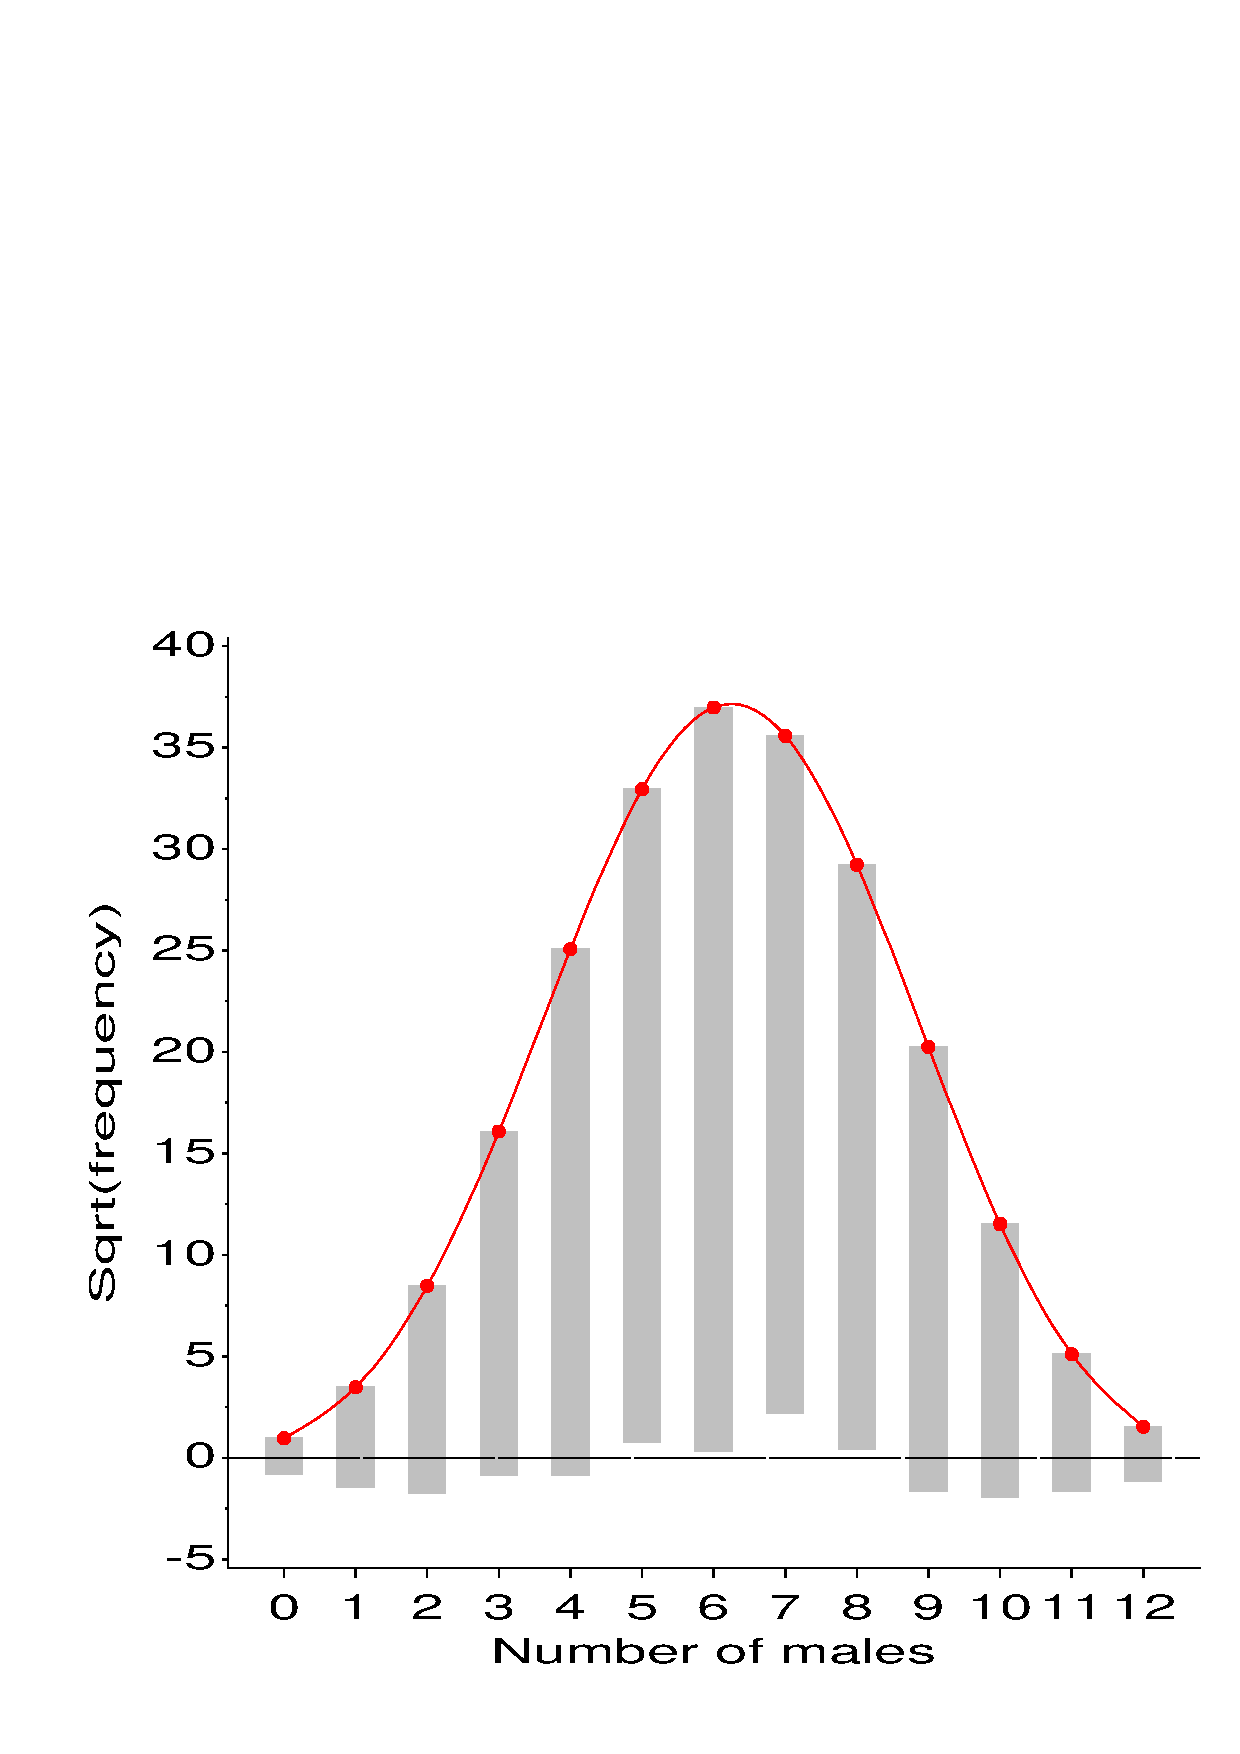
\includegraphics[width=1\linewidth]{saxony}\graphicsfile{ch2/fig/saxony.eps}{}
 \end{minipage}%
 \hfill
 \begin{minipage}[c]{.33\linewidth}
  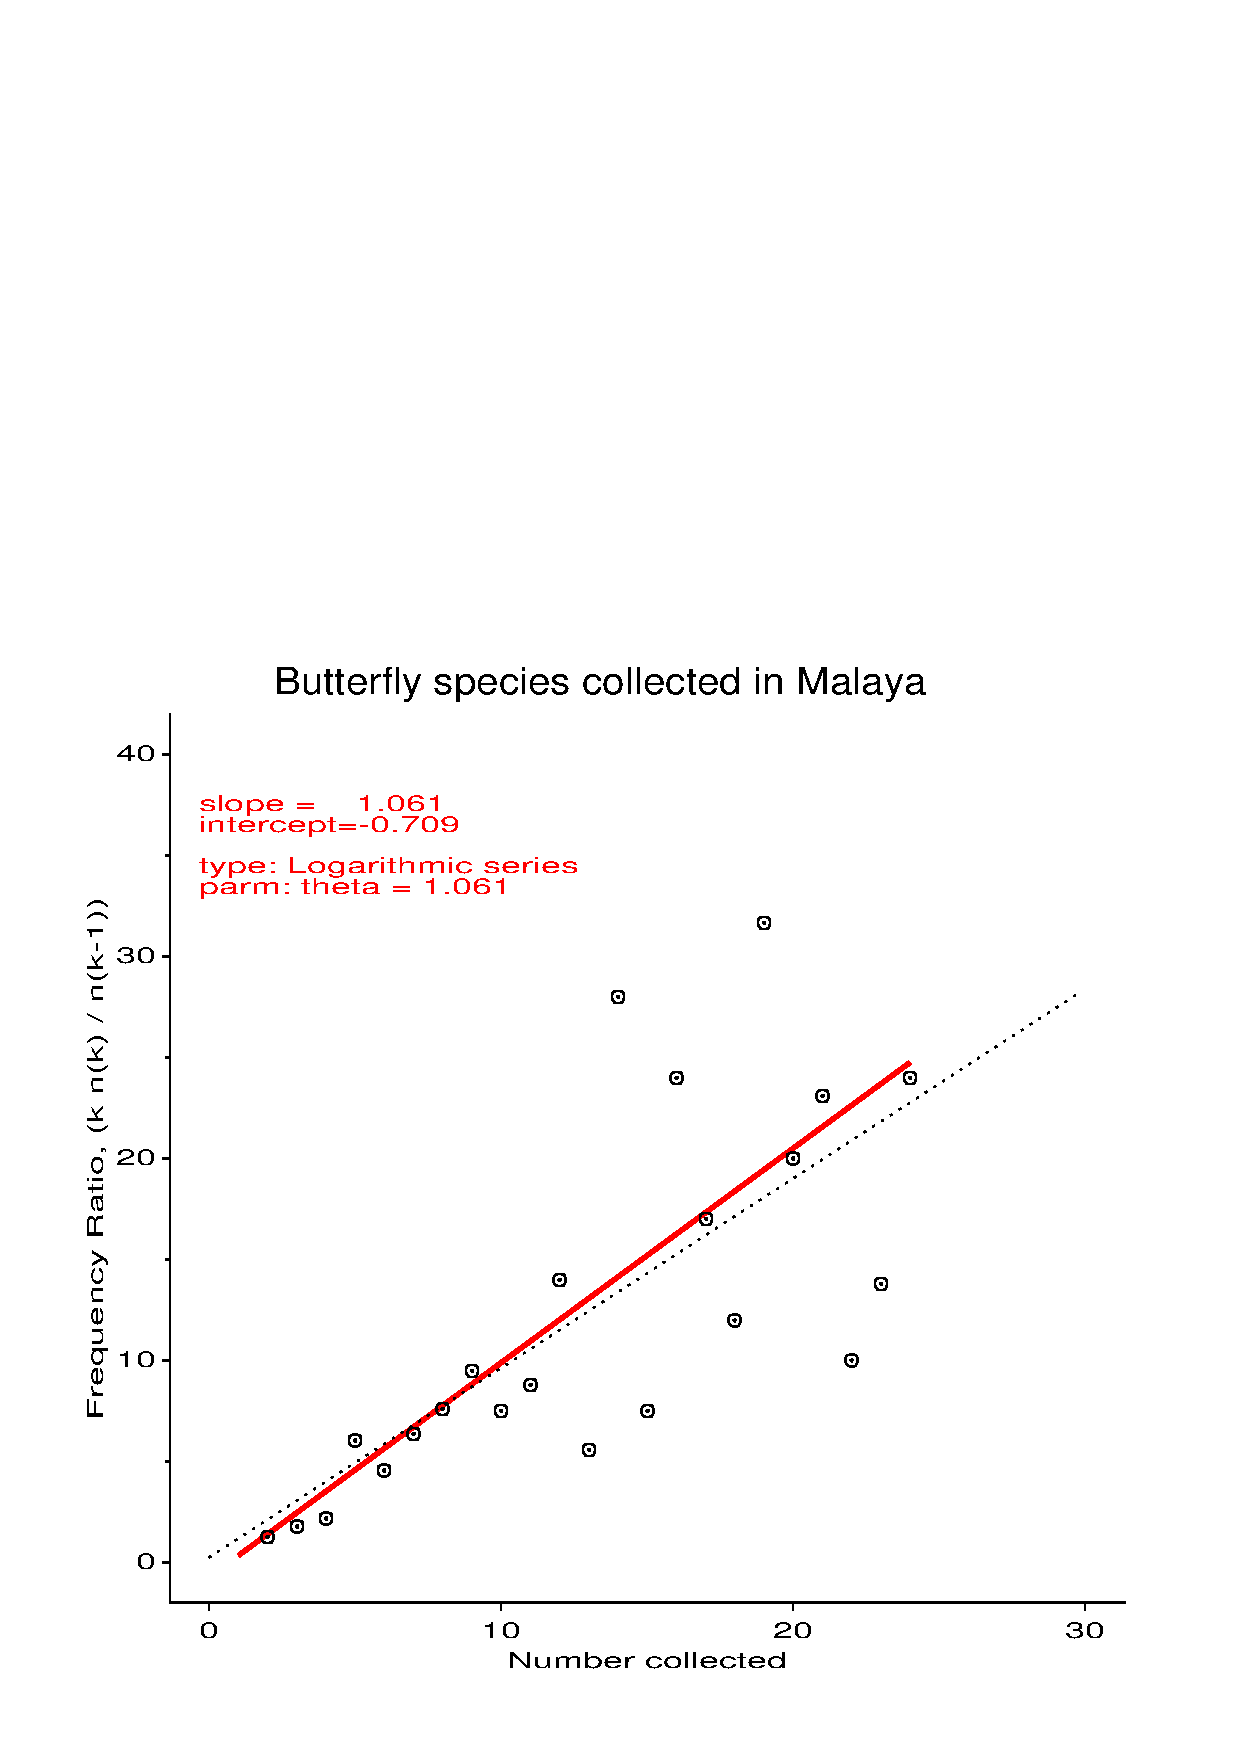
\includegraphics[width=1\linewidth]{orddemo3}\graphicsfile{ch2/fig/orddemo3.eps}{}
 \end{minipage}
 \hfill
 \begin{minipage}[c]{.33\linewidth}
  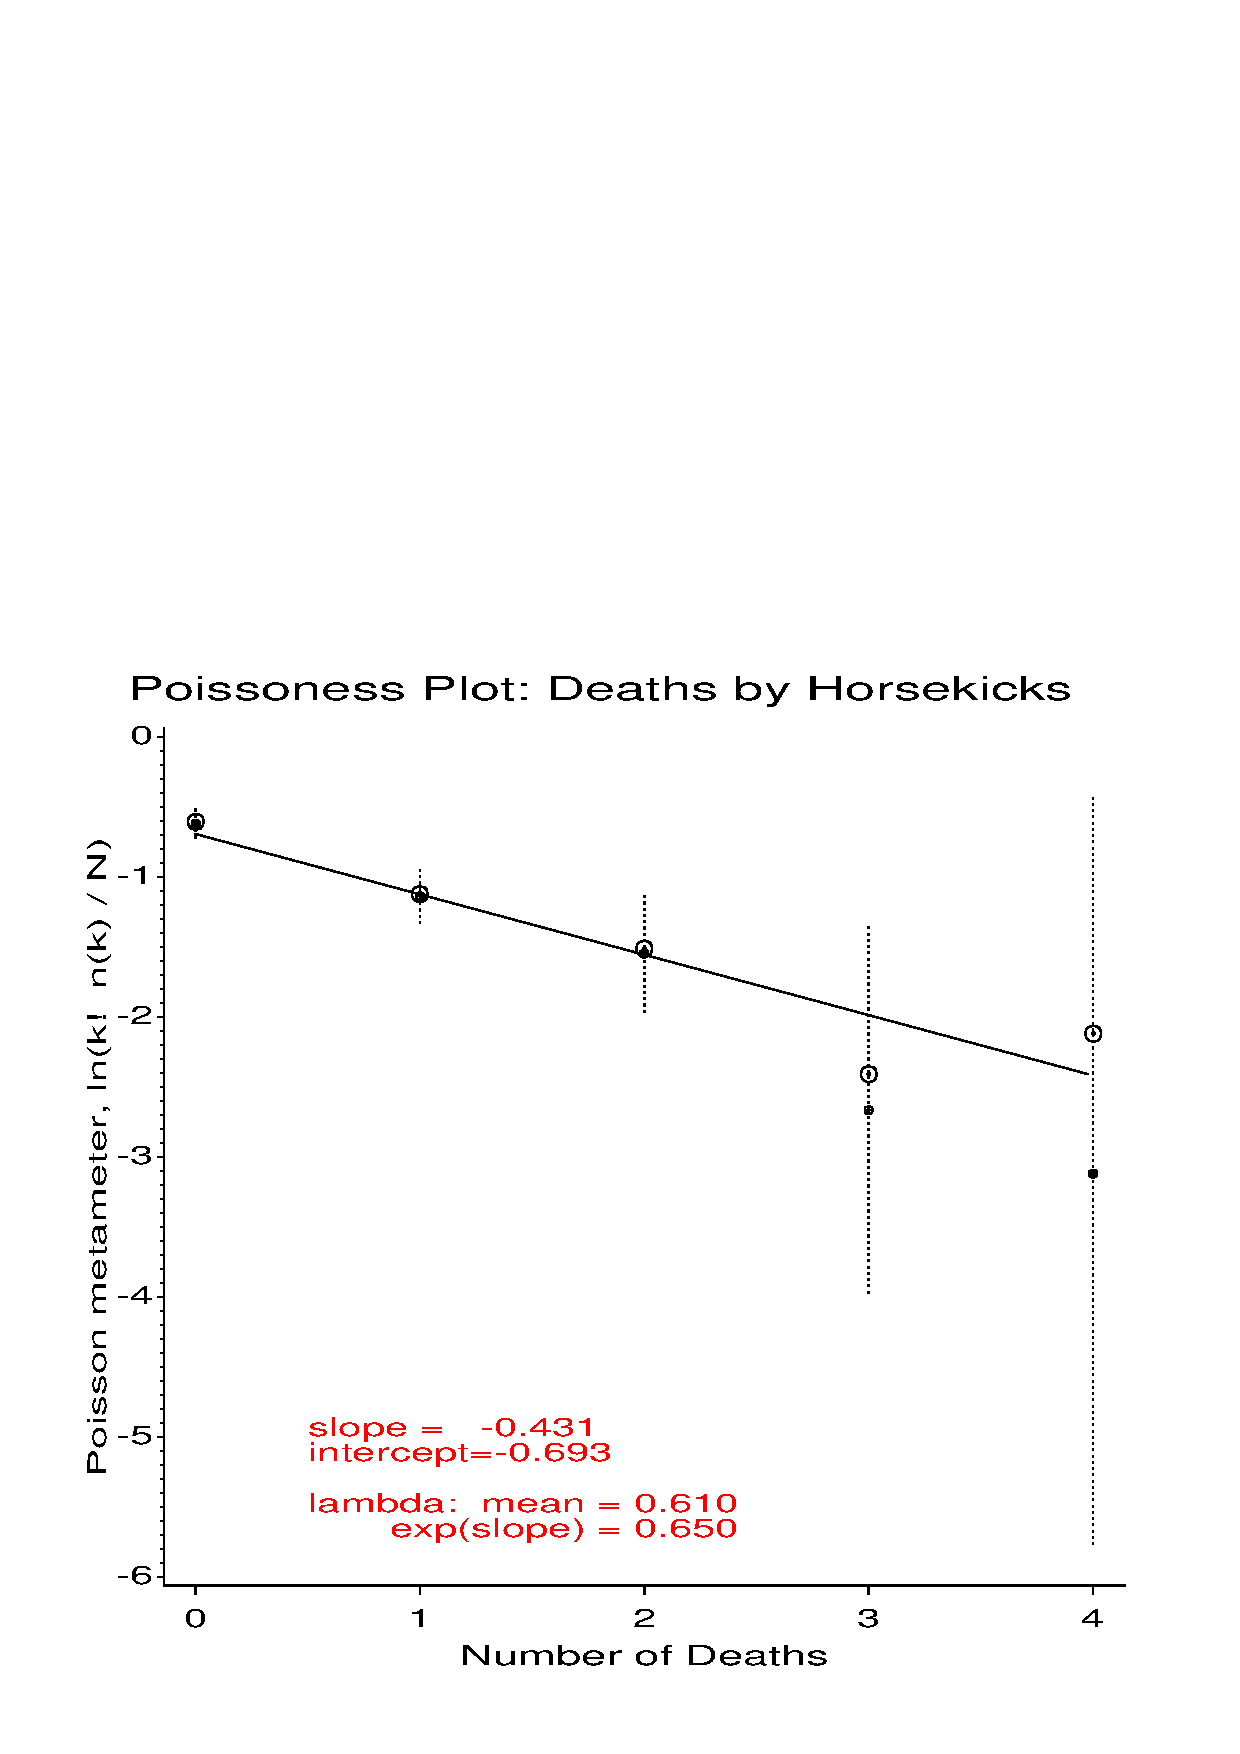
\includegraphics[width=1\linewidth]{poisdemo1}\graphicsfile{ch2/fig/poisdemo1.eps}{}
 \end{minipage}
\end{center}


\begin{quote}
{\Large
Discrete data often follow various theoretical probability models.
Graphic displays are used to visualize goodness of fit,
to diagnose an appropriate model, and determine the impact of
individual observations on estimated parameters.
}
\end{quote}
\minitoc
\clearpage

\section{Introduction}
\epigraph{Not everything that counts can be counted, and not everything that
can be counted counts.}
{Albert Einstein}
Discrete frequency distributions often involve counts of occurrences
such as accident fatalities, words in passages of text,  births of twins,
events of terrorism or suicide, or blood
cells with some characteristic.  Typically such data consist of a
table which records that \(n_k\) of the observations pertain to the
basic outcome value \(k \,  , \,  k = 0 , 1, \dots\).
For such data, we often wish to understand the process which gives rise to
these numbers, or to estimate frequencies for outcome values $k$ we
did not observe.  Both goals can be approached by examining
how closely the data follow a particular discrete probability distribution, such as the Poisson, the binomial, or the geometric distribution.

We briefly describe the properties of some of the most widely used
discrete distributions in \secref{sec:discrete-distrib}, along with
SAS techniques for calculating and visualizing those distributions.
\secref{sec:discrete-fit} presents theory and visualization techniques
related to fitting these distributions to empirical data.
In some cases, we may not know \emph{which} discrete distribution
should be fit to a given \Dset;  \secref{sec:discrete-Ord}
describes a simple graphical method designed to determine an appropriate
distribution type.
A more robust graphical method for diagnosing whether a given data
set follows the Poisson distribution is illustrated in \secref{sec:discrete-Poissonness}.
It turns out that the the discrete distributions described here
are members of a more general, parametric family, the \emph{power series},
permitting these
techniques to be applied to all of them.
A number of SAS macros to simplify the fitting and graphing of discrete
distributions are presented throughout the chapter.
  
The tables described in \exref{ex:horskick1}--\exref{ex:butterfly} illustrate several discrete data sets. For data such as these,
we can fit various discrete distributions and test hypotheses that
the fit is reasonably close.
However, rather than simply summarizing the goodness-of-fit in a
single number, we learn more from well-chosen graphical displays.

\begin{Example}[horskick1]{Death by horse kick}
One of the oldest and best known examples of a Poisson distribution
is the data from
\citet{Bortkiewicz:98} on deaths of soldiers in the Prussian
army from kicks by horses and mules, shown in \tabref{tab:horskick}.
von Bortkiewicz tabulated the number of soldiers in each of
14 army corps in the 20 years from 1875-1894
who died after being kicked by a horse
\citep[p. 18]{AndrewsHerzberg:85}.
\tabref{tab:horskick} shows the data used by
\citet{Fisher:25} for 10 of these
army corps, summed over 20 years, giving 200
`corps-year' observations.  In 109 corps-years,
no deaths occurred; 65 corps-years had one death, etc.
The data set is given more fully in \datref{dat:vonbort}.
The distribution is plotted in \figref{fig:poischart1}.
%% table from data set horskick (poistab.sas)
\begin{table}[htb]
\caption{Death by horse kicks}
\label{tab:horskick}
 \begin{center}
  \begin{tabular}{rr}
  \hline
Number of   & Number of  \\
Deaths ($k$)& Corps-Years ($n_k$)\\
  \hline
0 & 109 \\
1 & 65 \\
2 & 22 \\
3 & 3 \\
4 & 1 \\
  & N = 200 \\
  \hline
  \end{tabular}
 \end{center}
\end{table}

\end{Example}

\begin{Example}[madison1]{Federalist papers}
In 1787--88, Alexander Hamilton, John Jay, and James Madison
wrote a series of newspaper essays to persuade the voters of
New York State to ratify the U.S. Constitution.
The essays were titled \emph{The Federalist Papers}
and all were signed with the pseudonym ``Publius.''  Of the 77 papers published,
the author(s) of 65 are known, but \emph{both}
Hamilton and Madison later claimed sole authorship of the remaining 12.
\citet{MostellerWallace:84}
investigated the use of statistical methods to identify authors of
disputed works based on the frequency distributions of certain key
function words, and concluded that Madison had indeed authored the
12 disputed papers.  

\tabref{tab:madison} shows the distribution of the occurrence of one of
these ``marker'' words, 
the
word \emph{may} in 262 blocks of text (each about 200 words long)
from issues of the \emph{Federalist Papers} and other essays known
to be written by James Madison.  In 156 blocks, the word \emph{may}
did not occur; it occurred once in 63 blocks, etc.  The distribution
is plotted in \figref{fig:poischart2}.

%% table from data set madison (poistab.sas)
\begin{table}[htb]
\caption[Occurrences of `may' in Federalist Papers]{Number of Occurrences of the word \emph{may} in Federalist Papers
and essays written by James Madison}
\label{tab:madison}
 \begin{center}
  \begin{tabular}{rr}
  \hline
Number of        & Blocks of \\
Occurrences ($k$)& Text ($n_k$)\\
  \hline
0 & 156 \\
1 & 63 \\
2 & 29 \\
3 & 8 \\
4 & 4 \\
5 & 1 \\
6 & 1 \\
  & N = 262 \\
  \hline
  \end{tabular}
 \end{center}
\end{table}


\begin{figure}[htb]
 \begin{minipage}[b]{.5\linewidth}
  \centering
  \includegraphics[width=.9\linewidth,clip]{ch2/fig/poischart1.eps}
  \caption{von Bortkiewicz's data}\label{fig:poischart1}
 \end{minipage}%
 \begin{minipage}[b]{.5\linewidth}
  \centering
  \includegraphics[width=.9\linewidth,clip]{ch2/fig/poischart2.eps}
  \caption{Mosteller \& Wallace data}\label{fig:poischart2}
 \end{minipage}
\end{figure}

Note that the distributions of these data sets in \figref{fig:poischart1}
and \figref{fig:poischart2} are superficially similar in shape:
both have their mode at $k=0$ and frequencies $n_k$ which steadily
decline as $k$ increases.
Nevertheless, it turns out, the Horse Kick data is reasonably well-described by
a Poisson distribution, but the Madison data is not (Mosteller
and Wallace concluded that a negative binomial distribution provides
a better fit).
\end{Example}

Several other discrete distributions are illustrated by the
following examples.

\begin{Example}[queues]{Women in queues}
\citet{JinkinsonSlater:81,HoaglinTukey:85}
give the frequency distribution of the number of females observed in
queues of length 10 in a London Underground station.
If it is assumed that people line up independently, and that
men and women are equally likely to be found in a queue
(not necessarily reasonable assumptions),
then the number of women out of 10
would have a (symmetric) binomial distribution with parameters $N=10$ and
$p=\frac12$.
The frequency distribution, shown in \tabref{tab:queues},
appears systematically asymmetric, as we can see more clearly in
a histogram, \figref{fig:poischart3}.
However, there is no real reason to expect that males and females are
equally likely to be found in queues in the London underground,
so we may be interested in estimating $p$ from the data
and determining if a binomial distribution fits.

%% table from data set queues (poistab.sas) generated 16DEC97
\begin{table}[htb]
\caption{Number of women in 100 queues of length 10}
\label{tab:queues}
 \begin{center}
  \begin{tabular}{rr}
  \hline
Number of  & Number of \\
women ($k$) &  queues ($n_k$)\\
  \hline
0 & 1 \\
1 & 3 \\
2 & 4 \\
3 & 23 \\
4 & 25 \\
5 & 19 \\
6 & 18 \\
7 & 5 \\
8 & 1 \\
9 & 1 \\
10 & 0 \\
  & N=100 \\
  \hline
  \end{tabular}
 \end{center}
\end{table}


%% one figure
\begin{figure}[htb]
% \SASfig{poischart3.eps}{scale=.9}{poischart3}{Women in Queues of Length 10}
  \centering
  \includegraphics[scale=.9]{poischart3.eps}
  \caption{Women in Queues of Length 10}%
  \label{fig:poischart3}
\end{figure}
\end{Example}

\begin{Example}[dice]{Weldon's dice}
Common examples of binomial distributions involve tossing coins
or dice.
Perhaps the most industrious dice-tosser of all times,
Weldon tallied the results of throwing 12 dice 26,306 times
(a task which presumably required a good deal of leisure time).
He reported his results in a letter to Francis Galton dated
February 2, 1894, in order
``to judge whether the differences between a series of group frequencies
and a theoretical law \dots were more than might be attributed
to the chance fluctuations of random sampling''
\citep{KempKemp:91}.
In his seminal paper,
\citet{Pearson:00} used Weldon's data to illustrate the \chisq{} goodness-of-fit test, as did
\citet[Table 5.1, p. 121]{KendallStuart:63}.  These data are
shown here as
\tabref{tab:dice},
in terms of the number of occurrences of either a 5 or
6 in the throw of 12 dice.
If the dice were all identical and perfectly fair (balanced), one would
expect that $p = \Pr\{5 \textrm{ or } 6\} = \frac13$
and the distribution of the number of 5 or 6 would be binomial.
A peculiar feature of these data
as presented by Kendall and Stuart (not uncommon in discrete distributions)
is that the frequencies of 10--12 successes
are lumped together.  This grouping must be taken into account in fitting
the distribution.  The distribution is shown in \figref{fig:dice}.
%% table from data set dice (dice.sas) generated 26DEC97
\begin{table}[htb]
\caption{Frequencies of a 5 or 6 in throws of 12 dice}
\label{tab:dice}
 \begin{center}
  \begin{tabular}{rr}
  \hline
Number of  & Frequency \\
5s or 6s ($k$) & ($n_k$) \\
  \hline
0 & 185 \\
1 & 1149 \\
2 & 3265 \\
3 & 5475 \\
4 & 6114 \\
5 & 5194 \\
6 & 3067 \\
7 & 1331 \\
8 & 403 \\
9 & 105 \\
10+ & 18 \\
    & N=26306 \\
  \hline
  \end{tabular}
 \end{center}
\end{table}

%% one figure
\begin{figure}[htb]
%  \SASfig{dice.eps}{scale=.65}{dice}{Weldon's dice data}
  \centering
  \includegraphics[scale=.65]{dice.eps}
  \caption{Weldon's dice data}%
  \label{fig:dice}
\end{figure}
\end{Example}

\begin{Example}[butterfly]{Butterfly species in Malaya}
In studies of the diversity of animal species, individuals are
collected and classified by species.
The distribution of the number of species (types) where $k = 1, 2, \dots$
individuals (tokens) were collected forms a kind of type-token distribution.
An early example of this kind of distribution was presented by
\citet{Fisher-etal:43}.
\tabref{tab:butterfly} lists the number of individuals of each of
501 species of butterfly collected in Malaya.
There were thus 118 species for which just a single instance was found,
74 species for which two individuals were found,
down to 3 species for which 24 individuals were collected.
Fisher et-al.\  note however that the distribution was truncated
at $k = 24$.
Type-token distributions are often J-shaped, with a long upper tail,
as we see in \figref{fig:poischart4}.
%% table from data set butfly (poistab.sas) generated 11DEC97
\begin{table}[htb]
{
\small
\caption{Number of butterfly species for which $k$ individuals were collected}
\label{tab:butterfly}
 \begin{center}
  \begin{tabular}{rr|rr}
  \hline
Number of & Number of & Number of & Number of \\
Individuals ($k$)& Species ($n_k$) & Individuals ($k$)& Species ($n_k$)\\
  \hline
1 & 118 & 13 & 6 \\
2 & 74 & 14 & 12 \\
3 & 44 & 15 & 6 \\
4 & 24 & 16 & 9 \\
5 & 29 & 17 & 9 \\
6 & 22 & 18 & 6 \\
7 & 20 & 19 & 10 \\
8 & 19 & 20 & 10 \\
9 & 20 & 21 & 11 \\
10 & 15 & 22 & 5 \\
11 & 12 & 23 & 3 \\
12 & 14 & 24 & 3 \\
    & &   & N = 501 \\ 
  \hline
  \end{tabular}
 \end{center}
}
\end{table}


%% one figure
\begin{figure}[htb]
%  \SASfig{poischart4.eps}{width=.9\linewidth}{poischart4}{Butterfly species in Malaya}
  \centering
  \includegraphics[width=.9\linewidth]{poischart4.eps}
  \caption{Butterfly species in Malaya}%
  \label{fig:poischart4}
\end{figure}
\end{Example}

\section{Discrete distributions}\label{sec:discrete-distrib}
This section briefly reviews the characteristics of some of the
important discrete distributions encountered in practice.
For each distribution, we describe properties and generating
mechanisms, and show how its parameters can be estimated
and how to plot the frequency distribution.
For more detailed information on these and other discrete distributions,
\citet{Johnson-etal:92} present the most comprehensive treatment
and \citet[\C 2]{Zelterman:99} gives a compact summary.

\subsection{The binomial distribution}
\ix{binomial distribution|(}
The binomial distribution arises as the distribution of the
number of events of interest which occur in $n$ independent trials
when the probability of the event on any one trial is the constant
value $p = \Pr ( \textrm{event} )$.
For example, if 15\% of the population has red hair,
the number of red-heads in randomly sampled groups of $n=10$
might follow a binomial distribution, $\Bin(10, 0.15)$.
Over $n$ independent trials, the number of events  $k$
may range from 0 to $n$; if $X$ is a random variable
with a binomial distribution, the probability that $X = k$ is given
by

\begin{equation}\label{eq:binom}
\Bin(n,p): \Pr \{ X = k \} \equiv p ( k )  =
{n \choose k} p^k (1-p)^{n-k}
  \quad\quad k = 0, 1, \dots, n
  \comma
\end{equation}
where ${n \choose k} = n! / k! (n - k)!$ is the number of ways
of choosing $k$ out of $n$.
The first three (central) moments of the binomial distribution are
(letting $q = 1 - p$),
\begin{eqnarray*}
\textrm{Mean}[X] & = & n p  \\
\textrm{Var}[X] &  = & n p q \\
\textrm{Skew}[X] & = & n p q (q - p) 
\comma
\end{eqnarray*}
so the binomial distribution has its maximum variance and is
symmetric when $p = .5$.

If we are given data in the form of a discrete (binomial) distribution
(and $n$ is known),
then the maximum likelihood estimator of $p$ can be obtained
as
\begin{equation*}% \label{eq:binp}
\hat{p} = \frac{\bar{x}}{n} =
  \frac{(\sum_{k} k \times n_k ) / \sum_k n_k}{n}
  \comma
\end{equation*}
with sampling variance $pq/n$.

\subsubsection{Calculation and visualization}
\ix{binomial distribution!visualization|(}
In SAS you can calculate binomial probabilities \eqref{eq:binom} with the
\FUNC{probbnml} and generate random data from a binomial
distribution with the \FUNC{ranbin} or the \CALL{ranbin}.
The \FUNC{probbnml},
\texttt{probbnml(p,n,m)} calculates cumulative probabilities,
$ \sum_{k=0}^{k=m} p ( k )$,
so to find individual probability densities, you must subtract
successive values for $k$ and $k-1$.
In \sasver{6.12} and above, the general \FUNC{pdf}
calculates probability densities directly, for the binomial
and most other distributions.  For the binomial distribution,
it is called as \texttt{pdf('binomial',m,p,n)}.

Discrete distributions are easily visualized by plotting the probability
density (or expected frequencies in a total sample of given size)
against the random variable ($k$), for given values of the distribution
parameters.

For example, assume that 15\% of the population has red
hair, and 35\% has brown hair.
What are the probabilities that in groups of $n=10$
people, $k = 0, 1, \dots, 10$ will have red hair or brown
hair, respectively?
We can calculate these probabilities
(and the expected frequencies in 1000 repetitions) in a \Dstp{} as
follows, giving the output in \outref{out:binomial1}.
We use macro variables for $n$ and $p$ (in the form of a \texttt{DO} list)
so that the same program may be
used for any binomial distributions.
A complete distribution is generated for each combination of $n$ and $p$.

%% input: /users/faculty/friendly/sasuser/catdata/binomial.sas
%% last modified: 22-Dec-97  9:44
\begin{listing}
%let N=10;
%let p=.15, .35;
title "Binomial distributions, N=&N, p=&p";
data binomial;
   reps = 1000;
   drop reps;
   N=&N;
   do p=&p;
      do k=0 to N;
         if k=0 
            then prob = probbnml(p, N, 0);
            else prob = probbnml(p, N, k) - probbnml(p, N, k-1);
         freq = reps * prob;
         output;
         end;
      end;
   label freq='Frequency'
      k = 'k';
proc print;
   id p;
   by p;
run;

proc means data=binomial mean var max vardef=weight;
   var k;
   weight prob;
   by p;
\end{listing}


\begin{Output}
\caption{Binomial probabilities}\label{out:binomial1}
\verbatiminput{ch2/out/binomial1.out}
\end{Output}

\begin{Output}
\caption{Means and variances for binomial probabilities}\label{out:binomial2}
\verbatiminput{ch2/out/binomial2.out}
\end{Output}

Notice that in the \PROC{MEANS} step the option \texttt{VARDEF=WEIGHT}
is used to calculate the variance correctly from a grouped frequency distribution,
producing the output in \outref{out:binomial2}.
These distributions are shown side-by-side in \figref{fig:binomial},
plotted using \PROC{GCHART}, with $p$ as a group variable:
\begin{listing}
proc gchart data=binomial;
   vbar k /sumvar=freq group=p midpoints=0 to 10
      coutline=black frame raxis=axis1;
   pattern1 v=solid c=grayc0;
   axis1 order=(0 to 350 by 50);
run; quit;
\end{listing}

%% one figure
\begin{figure}[htb]
%  \SASfig{binomial.eps}{scale=.75}{binomial}{Binomial distributions for $n=10$ trials}
  \centering
  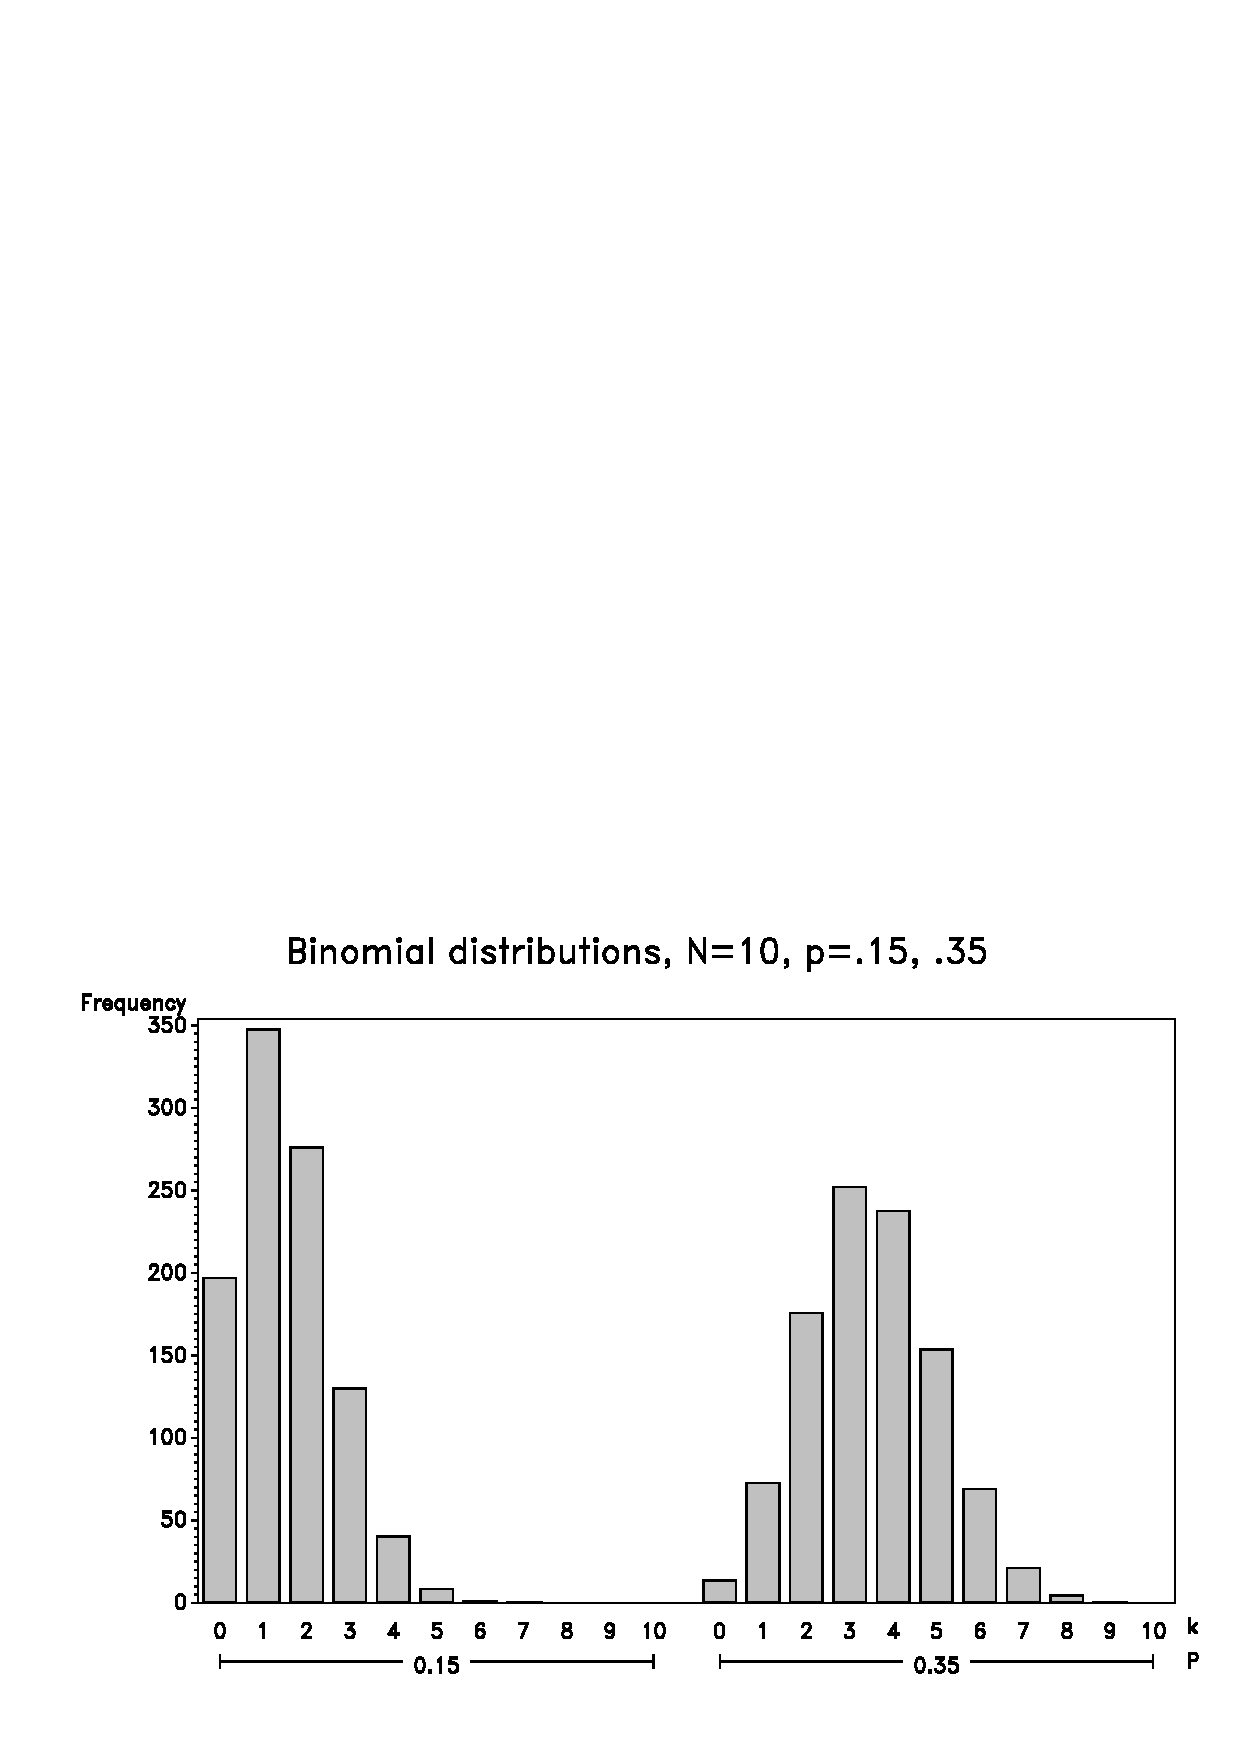
\includegraphics[scale=.75]{binomial}\graphicsfile{ch2/fig/binomial.eps}{}
  \caption{Binomial distributions for $n=10$ trials}%
  \label{fig:binomial}
\end{figure}
Alternatively, one may prefer to plot such distributions as frequency
polygons or as needle graphs, using \PROC{GPLOT}.
For example, \figref{fig:binomial2} shows frequency polygons for
the binomial distributions $\Bin(10,p)$ with $p = 0.15 (0.20) 0.75$,
obtained by running the \texttt{binomial} \Dstp\ with
\begin{listing}
%let p=.15 to .75 by .20;
\end{listing}
The \PROC{GPLOT} step (excluding statements for symbols, axes, and the
legend) is just
\begin{listing}
proc gplot data=binomial;
   plot freq * k = p / frame vminor=1 hminor=0 ... ;
\end{listing}

%% one figure
\begin{figure}[htb]
%  \SASfig{binomial2.eps}{scale=.75}{binomial2}{Binomial distributions for $n=10$ trials, as frequency polygons}
  \centering
  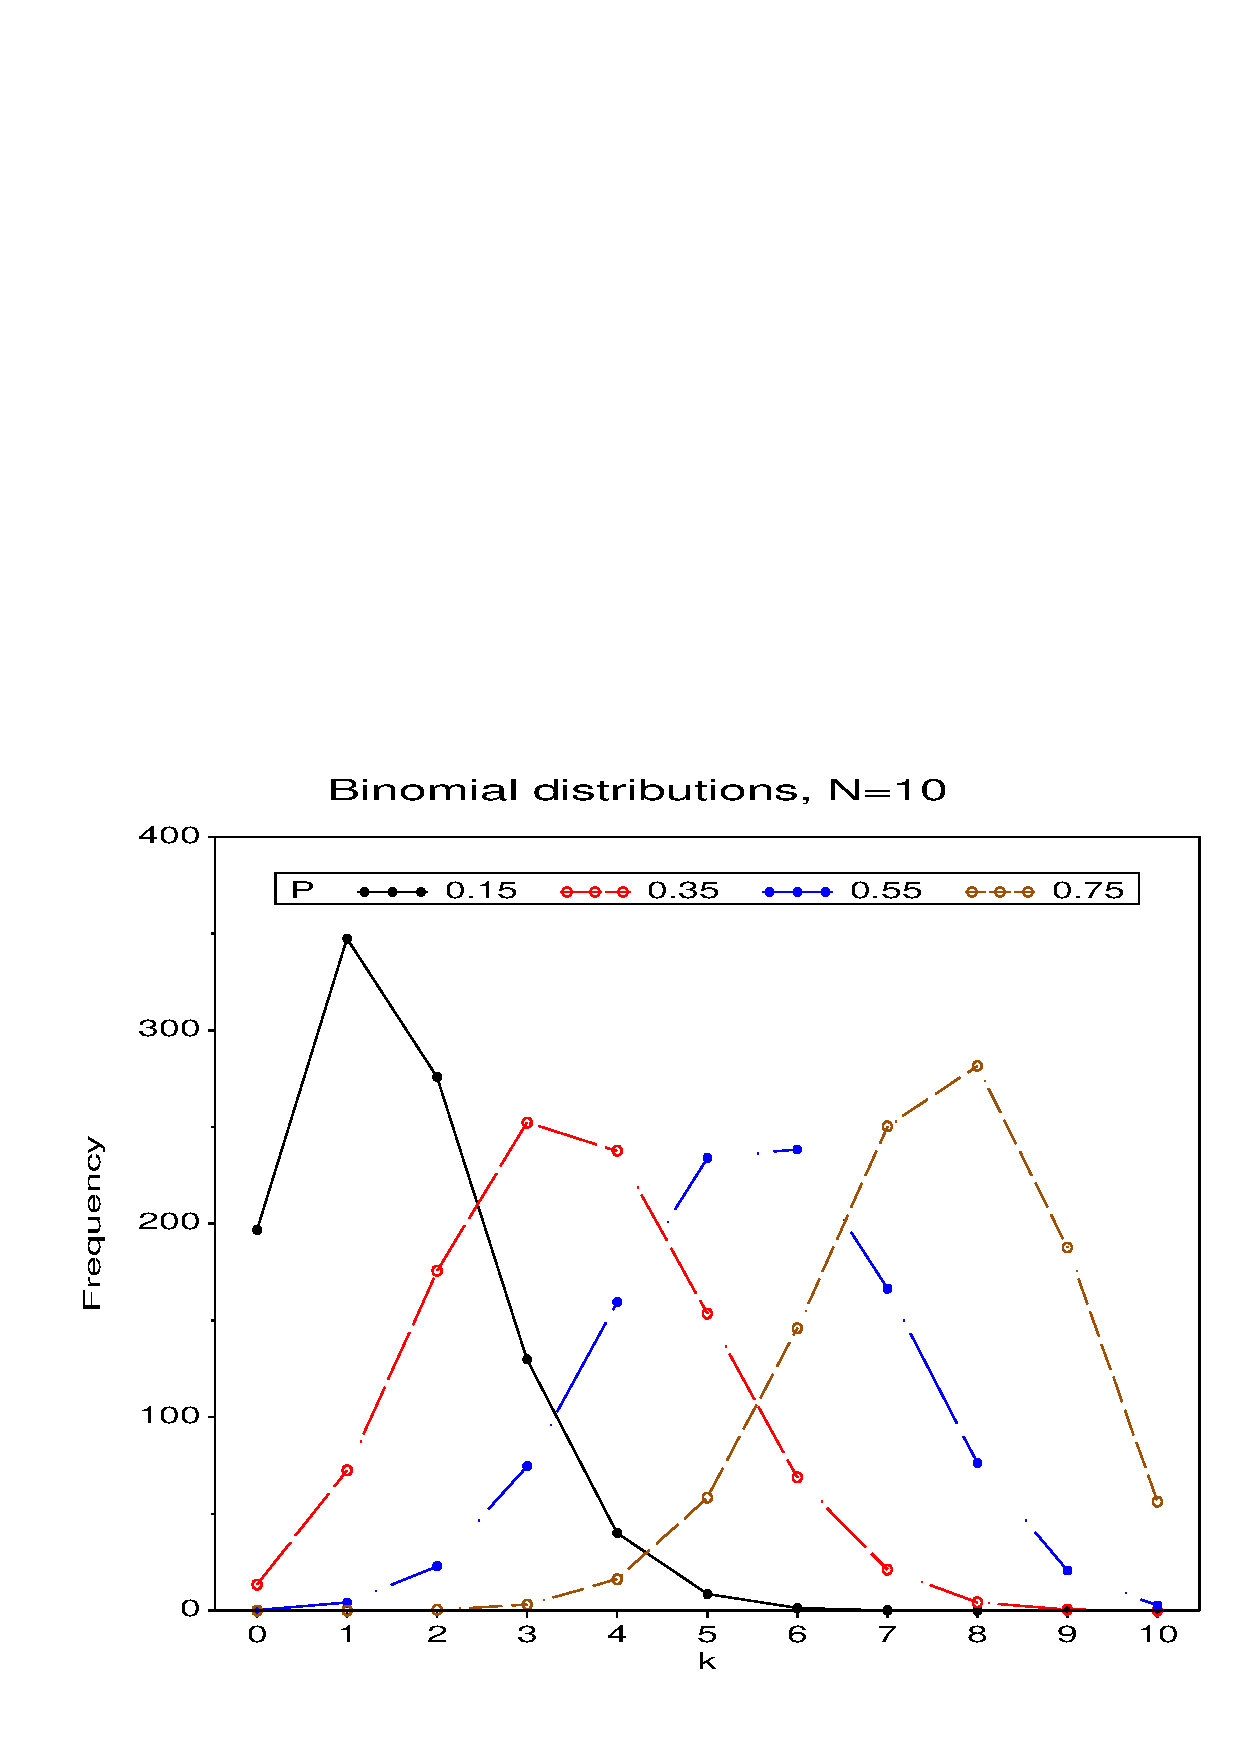
\includegraphics[scale=.75]{binomial2}\graphicsfile{ch2/fig/binomial2.eps}{}
  \caption{Binomial distributions for $n=10$ trials, as frequency polygons}%
  \label{fig:binomial2}
\end{figure}
\ix{binomial distribution!visualization|)}
\ix{binomial distribution|)}

\subsection{The Poisson distribution}
\ix{Poisson distribution|(}

The Poisson distribution gives the probability of an event occurring
$k = 0, 1, 2, \dots$ times over a large number of ``trials'',
when the probability, $p$, that the event occurs on any one
trial is very small and constant;
hence, the Poisson distribution is usually applied to the study of
rare events such as highway accidents at a particular location,
deaths from horse kicks, or defects in a well-controlled manufacturing
process.

For the \IX{Poisson distribution}, the probability function
is
\begin{equation}\label{eq:poisf}
\textrm{Pois}(\lambda):\Pr \{ X = k \} \equiv p (k)=
  \frac{ e^{ - \lambda } \:  \lambda^k } { k ! }
  \quad\quad k = 0, 1, \dots
\end{equation}
where the parameter, $\lambda$ turns out to be the mean of the
distribution.
The first three (central) moments of the Poisson distribution are
in fact all equal to $\lambda$:
\begin{eqnarray*}
\textrm{Mean}[X] & = & \lambda \\
\textrm{Var}[X] &  = & \lambda \\
\textrm{Skew}[X] & = & \lambda 
\end{eqnarray*}
%% Mathematica gives Skew = 1 / \sqrt(\lambda) ???

So, the mean and variance of the Poisson distribution are always
the same, which is sometimes used to identify a distribution
as Poisson.  For the binomial distribution, the mean ($Np$) is always
greater than the variance ($Npq$); for other distributions
(negative binomial and geometric) the mean is less than the
variance.

The maximum likelihood estimator of the parameter \(\lambda\)
in \eqref{eq:poisf} is just
the mean of the distribution,
\begin{equation*}
  \hat{\lambda}= \bar{x} = \frac{\sum_k k \,  n_k}{\sum_k  n_k}
  \period
\end{equation*}
Hence, the expected frequencies can be estimated by substituting the
sample mean into \eqref{eq:poisf}.
Moreover, Poisson variables have a nice reproductive property:
 if $X_1, X_2, \dots X_m$ are independent Poisson
variables with the same parameter $\lambda$, then their
sum, $\sum X_i$ is a Poisson variate with parameter $m \lambda$;
if the Poisson parameters differ, the sum is still Poisson with
parameter $\sum \lambda_i$.

\begin{Example}[soccer]{UK Soccer scores}
\tabref{tab:soccer1}  gives the distributions of goals scored by
the 20 teams in the  1995/96 season of the
 Premier League of the UK Football Association
as presented by
\citet{Lee:97}.%
\footnote{\citet[p. 16]{Lee:97} apparently has the home and away labels reversed in
his table.
The row and column labels in \tabref{tab:soccer1} give means of 1.48
for home teams and 1.06 for away teams.  The raw data were verified
from that listed at \url{http://users.aol.com/mabstabs/soccer.html}}
Over a season
each team plays each other team exactly once, so there are a total of
$20 \times 19 = 380$ games.
Because there may be an advantage for the home team,
the goals scored have been classified as ``home team'' goals
and ``away team'' goals in the table.
\input{ch2/tab/soccer1}

If we assume that in any small interval of time there is a small, constant
probability that the home team or the away team may score a goal,
the distributions of the goals scored by home teams
(the row totals in \tabref{tab:soccer1})
may be modeled as Pois($\lambda_H$) and the distribution of
the goals scored by away teams (the column totals)
may be modeled as Pois($\lambda_A$).

If the number of goals scored by the home and away teams are independent%
\footnote{This question
is examined visually in \chref{ch:mosaic} (\exref{ex:soccer2})
and \chref{ch:corresp} (\exref{ex:soccer3}), where we find that the answer
is ``basically, yes''.},
we would expect that the total number of goals scored in any
game would be distributed as Pois($\lambda_H + \lambda_A$).
These totals are shown in \tabref{tab:soccer2}.
As preliminary check of the distributions for the home and away goals,
we can determine if the means and variances are reasonably close
to each other.
If so, then the total goals variable should also have a mean and variance
equal to the sum of those statistics for the home and away goals.
\input{ch2/tab/soccer2}

The statements below read the data from \tabref{tab:soccer1}, calculate
the \texttt{TOTAL} goals, and find the distribution of \texttt{TOTAL} goals
shown in \tabref{tab:soccer2}.  The \PROC{MEANS} step produces the
mean and variance of each variable, shown in \outref{out:soccer1.2}.
\input{ch2/sas/soccer1}

\begin{Output}[htb]
\caption{UK Soccer data, assessing Poissonness}\label{out:soccer1.2}
\small
\verbatiminput{ch2/out/soccer1.2}
\end{Output}
The means are all approximately equal to the corresponding variances.
More to the point, the variance of the \texttt{TOTAL} score
is approximately equal to the sum of the individual variances.
Note also there does appear to be an advantage for the home team,
of nearly half a goal.
\end{Example}


\subsubsection{Calculation and visualization}
\ix{Poisson distribution!visualization|(}
Poisson probabilities may be calculated using the \FUNC{poisson},
which is called as \texttt{poisson(lambda, m)} for a distribution
with mean \texttt{lambda}.
This also returns cumulative probabilities,
$ \sum_{k=0}^{k=m} p ( k )$,
which must be differenced to calculate the probability of exactly
$m$ events.  The \FUNC{pdf}, called as \texttt{pdf('poisson', m, lambda)}
calculates these densities directly.
Random data from a poisson distribution may be obtained using the
\CALL{ranpoi}.

The \Dstp\ below illustrates the use of the \FUNC{pdf} to calculate
poisson frequencies for the distributions with means ($\lambda$) 2 and 5,
for $k = 0, 1, \dots , 12$.

%% input: /Users/friendly/sasuser/catdata/poisson1.sas
%% last modified: 07-Jul-99 13:37
\begin{listing}
%let N=12;
%let lambda = 2, 5;
title "Poisson distributions, lambda=&lambda, k=0..&N";
data poisson;
   reps = 1000;
   drop reps;
   N=&N;
   do lambda=&lambda;
      do k=0 to N;
         prob = pdf('poisson', k, lambda);
         freq = reps * prob;
         output;
         end;
      end;
   label freq='Frequency'
        lambda='Lambda'
        k = 'k';
\end{listing}

\begin{figure}[htb]
  \centering
  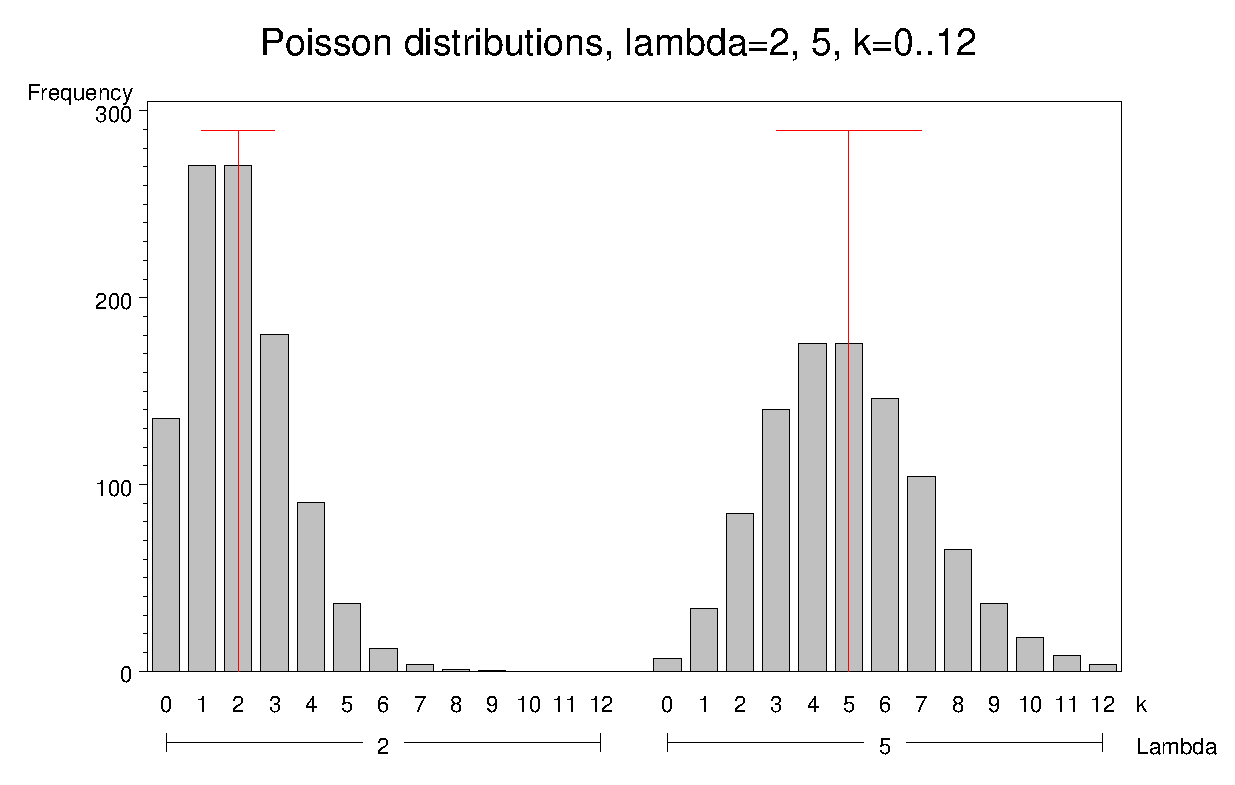
\includegraphics[scale=.75]{poisson1}\graphicsfile{ch2/fig/poisson1.eps}{}
  \caption[Poisson distributions with $\lambda =$ 2, 5.]{Poisson distributions with $\lambda =$ 2 and 5.  The vertical line shows the mean
  of each distribution; the horizontal lines show the standard deviation.}%
  \label{fig:poisson1}
\end{figure}

These distributions are shown in \figref{fig:poisson1},
plotted using \PROC{GCHART} as shown earlier for the binomial
distribution.
\ix{Poisson distribution!visualization|)}
\ix{Poisson distribution|)}

\subsection{The negative binomial distribution}
\ix{negative binomial distribution|(}

The negative binomial distribution is a type of waiting-time distribution.
One form of
the negative binomial distribution
(also called the Pascal distribution) arises when a series of Bernoulli
trials is observed with constant probability $p$ of some event,
and we ask how many trials it takes to observe
$n$ events.
The probability function with parameters $n$ (an integer, $0 < n < \infty$) and $p \, (0 < p < 1)$
gives the probability that $k$ non-events (failures) are observed before
the $n$-th event (success), and
can be written
\begin{equation}\label{eq:negbinf}
\NBin(n,p):   \Pr \{ X = k \} \equiv p(k)  =
  {n+k-1 \choose k} p^n (1-p)^k
  \quad\quad k = 0, 1, \dots , \infty
\end{equation}

The moments of the negative binomial distribution are:
\begin{eqnarray*}
\textrm{Mean}[X] &=&nq / p \\
\textrm{Var}[X] &=&nq / p^2 \\
\textrm{Skew}[X] &=&\frac{2-p}{\sqrt{nq}}
\comma
\end{eqnarray*}
where $q=1-p$.

A more general form of the negative binomial distribution
allows $n$ to take non-integer values and to be an unknown
parameter.
In this case, the combinatorial coefficient,
${n+k-1 \choose k}$ in \eqref{eq:negbinf} is calculated using
the gamma function, $\Gamma(\bullet)$,
a generalization of the factorial for non-integer values,
defined so that $\Gamma(x+1) = x!$ when $x$ is an integer.
Then the probability function \eqref{eq:negbinf} becomes
\begin{equation}\label{eq:negbinf2}
  \Pr \{ X = k \} \equiv p(k)  =
  \frac{\Gamma(n+k)}{\Gamma(n) \Gamma(k+1)}
   p^n (1-p)^k
  \quad\quad k = 0, 1, \dots , \infty
  \period
\end{equation}

In this form, the negative binomial distribution is frequently used
as an alternative to the Poisson distribution when the assumptions
of the Poisson (constant probability and independence) are not
satisfied, or when the variance of the distribution is greater
than the mean (termed \glossterm{overdispersion}).
\citet{GreenwoodYule:20}
developed the negative binomial distribution as a model for
accident proneness or susceptibility of individuals to
repeated attacks of disease.
They assumed that for any individual the number of accidents
or disease occurrences has a Poisson distribution with parameter
$\lambda_i$.
If individuals vary in proneness, so that the $\lambda_i$ have
a gamma distribution, the resulting distribution is the
negative binomial.

When both $n$ and $p$ are treated as unknown parameters,
maximum likelihood estimators are available, but involve
complex non-linear equations.
The simpler method of moments estimators
are
\begin{eqnarray*}
  \hat{p} & = & \bar{x} / s^2 \\
  \hat{n} & = & \bar{x}^2 / ( s^2 - \bar{x} )
  \comma
\end{eqnarray*}
where $\bar{x}$ and $s^2$ are the sample mean and variance of the observed
distribution.
Note that if $s^2 < \bar{x}$, the estimate of $n$ will be negative
and that of $p$ will be greater than 1, so the negative binomial
distribution should be considered inappropriate.

\subsubsection{Calculation and visualization}
The SAS \FUNC{probnegb} calculates negative binomial cumulative probabilities for
integer values of the number of successes parameter, $n$.
To calculate probabilities for individual values of $k$, it is necessary
to compute the difference between successive values $k-1$ and $k$,
as with the binomial and Poisson distribution functions,
or use the \FUNC{pdf}, called as \texttt{pdf('negbinomial', k, p, n)}.
For non-integer values of $n$ it is necessary to calculate the probabilities
directly using \eqref{eq:negbinf2}.
Random values from a negative binomial distribution may be obtained by
calculating the probabilities, $p(k), k=0, 1, \dots$ and
using these with the \FUNC{rantbl}.

\figref{fig:probnegb} shows negative binomial distributions for the number of
trials to observe  $n=2$ or $n=4$ successes with $p = .2, .3, .4$, and
with values of $k$ from 0 to 20.
The vertical line in each panel marks the location of the mean; the horizontal
line shows the range of one standard deviation about the mean.

%% one figure
\begin{figure}[htb]
% \SASfig{probnegb.eps}{scale=.8}{probnegb}{Negative binomial distributions for the number of trials to observe  {\protect{$n=2$ or $n=4$} successes}}
  \centering
  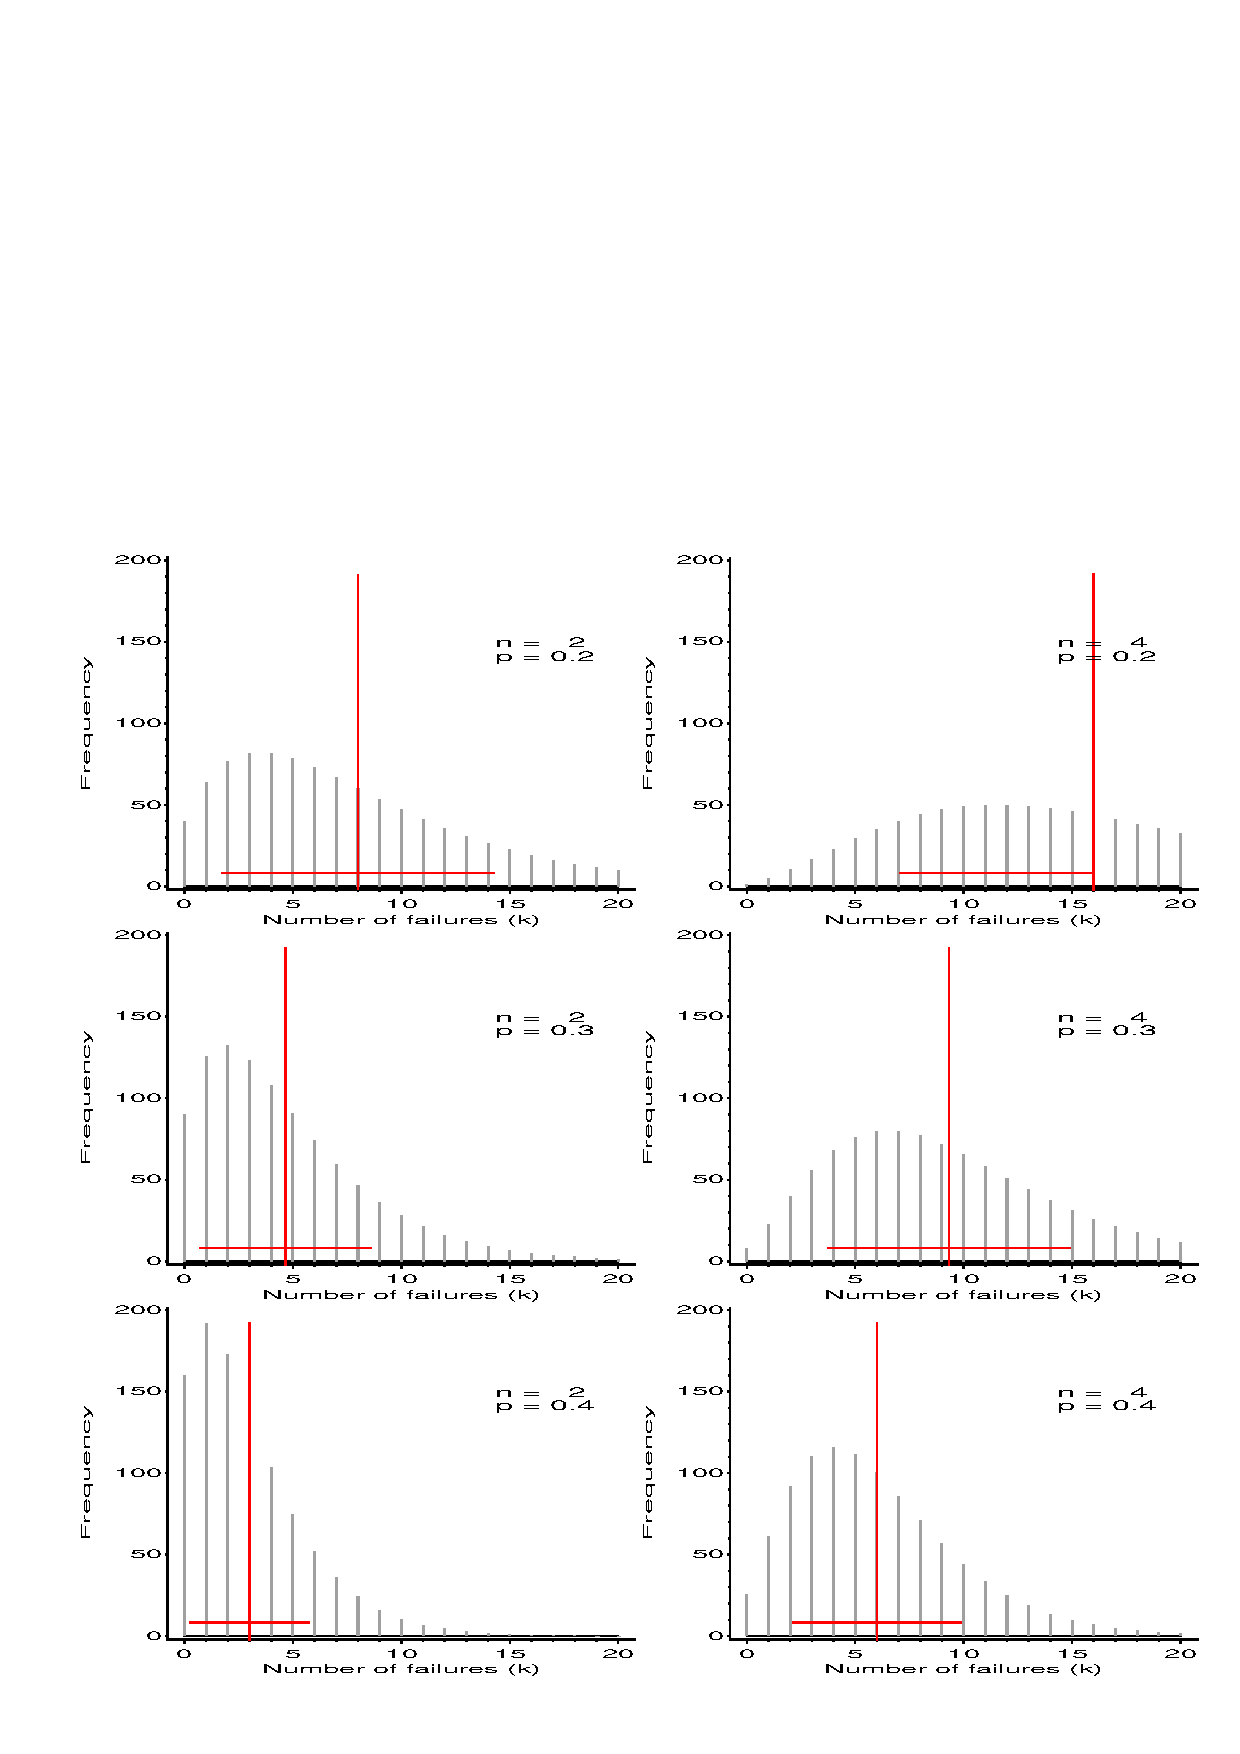
\includegraphics[scale=.8]{probnegb}\graphicsfile{ch2/fig/probnegb.eps}{}
  \caption{Negative binomial distributions for
        the number of trials to observe {\protect{$n=2$ or $n=4$} successes}}%
  \label{fig:probnegb}
\end{figure}
\ix{negative binomial distribution|)}

\subsection{The geometric distribution}
\ix{geometric distribution|(}
The special case of the negative binomial distribution when $n=1$
is a geometric distribution.
We observe a series of independent trials and count the number
of non-events (failures) preceding the first successful event.
The probability that there will be  $k$ failures before the first
success
is given by
\begin{equation}\label{eq:geomf}
\textrm{Geom}(p):   \Pr \{ X = k \} \equiv p ( k )  =
   p (1-p)^k
  \quad\quad k = 0, 1, \dots
  \period
\end{equation}
For this distribution,
\begin{eqnarray*}
\textrm{Mean}[X] & = & 1 / p\\
\textrm{Var}[X] &  = & (1-p) / p^2 \\
\textrm{Skew}[X] & = & (2-p) / \sqrt{1-p}
\end{eqnarray*}
\ix{geometric distribution|)}

\subsection{The logarithmic series distribution}
\ix{logarithmic series distribution|(}
The logarithmic series distribution is a long-tailed distribution
introduced by
\citet{Fisher-etal:43}
in connection with data on the abundance of individuals
classified by species of the type shown for the distribution of butterfly
species
in \tabref{tab:butterfly}.

The probability distribution function with parameter $\theta$ is given by
\begin{equation}\label{eq:logseriesf}
\textrm{LogSer}(\theta): \Pr \{ X = k \} \equiv p ( k )  =
\frac{\theta ^k}{-(k\log (1-\theta ))} =
\alpha \theta^k / k
\quad\quad k = 1, 2, \dots, \infty
\comma
\end{equation}
where $\alpha = -1 / \log(1 - \theta)$
and $0 < \theta <1$.
Fisher derived the logarithmic series distribution by assuming that
for a given species the number of individuals trapped has a Poisson
distribution with parameter $\lambda = \gamma t$, where
$\gamma$ is a parameter of the species (susceptibility to entrapment)
and $t$ is a parameter of the trap.
If different species vary so that the parameter $\gamma$ has a gamma
distribution, then the number of representatives of each species trapped
will have a negative binomial distribution.
However, the observed distribution is necessarily truncated on the left,
because one cannot observe the number of species never caught (where $k=0$).
The logarithmic series distribution thus arises as a limiting form of the
zero-truncated negative binomial.

From \eqref{eq:logseriesf}
\begin{equation*}
\frac{p(k+1)}{p(k)} = \frac{k \theta}{k+1} < 1
\comma
\end{equation*}
for all $k$, since $\theta < 1$.  Hence, the maximum probability occurs at $k=1$
and $p(k)$ decreases steadily as $k$ increases.

The mean and variance of the distribution are
\begin{eqnarray}
\textrm{Mean}[X] & = & \alpha \theta / (1-\theta ) \equiv \mu \label{eq:logsermean}\\
\textrm{Var}[X] & = &  \alpha \theta (1-\alpha\theta) / (1-\theta )^2
= \mu ( \frac{1}{1-\theta} - \mu )
\nonumber
\end{eqnarray}

In fitting this distribution to data, the method of moments and maximum likelihood
both involve equating the sample mean to the population mean in \eqref{eq:logsermean},
a nonlinear equation which must be solved numerically for $\theta$.
When $\bar{x} < 25$, an approximation given by
\citet{Birch:63},
\begin{equation*}%\label{eq:thetabirch}
\hat\theta  \approx
1 - \frac{1}{1 + [ ( \frac{5}{3} - \frac{1}{16}\log \bar{x}) (\bar{x}-1) + 2 ] \log \bar{x} }
\period
\end{equation*}

Another useful unbiased approximation is based on the proportion of observations
at $k=1$,
\begin{equation*}
\hat\theta  \approx 1- \frac{n_1 / N}{\bar{x}}
\period
\end{equation*}
\ix{logarithmic series distribution|)}

\subsection{Power series family}\label{sec:pwrseries}
\ix{power series distributions|(}

I mentioned earlier that the Poisson distribution was unique among all discrete (one parameter) distributions, in that it is the only one whose mean and variance are equal
\citep{Kosambi:49}.
The relation between mean and variance of discrete distributions also provides
the basis for integrating them into a general family.
All of the discrete distributions described in this section are in fact
special cases of a family of discrete distributions
called the power series distributions by
\citet{Noack:50}
and defined by
\begin{equation*}
p(k) = a(k) \theta^k / f(\theta)
\quad\quad k=0, 1, \dots \comma
\end{equation*}
with parameter $\theta > 0$,
where $a(k)$ is a coefficient function depending only on $k$
and $f ( \theta) = \sum_k a(k) \theta^k$ is called the series
function.  The definitions of these functions are shown in
\tabref{tab:pwrseries}.
\begin{table}[!tb] \centering%
\caption{The Power Series family of discrete distributions\label{tab:pwrseries}}%
\small
\begin{tabular}{lllll}\hline
Discrete & Probability  & Series  & Series  & Series \\ 
Distributiion & function, $p(k)$ & parameter, $\theta$ &
function, $f(\theta )$ & coefficient, $a(k)$ \\ \hline
%
Poisson & $e^{-\lambda }\lambda ^k/k!$ & $\theta = \lambda$ & $e^\theta $ & $1/k!$ \\[1ex] 
Binomial & $\binom nkp^k(1-p)^{n-k}$ & $\theta = p / (1-p) $ & $(1+\theta )^n$ & $\binom nk$ \\[1ex] 
Negative binomial & $\binom{n+k-1}kp^n(1-p)^k$ &  $\theta = (1-p) $ & $(1-\theta )^{-k}$ & $%
\binom{n+k-1}k$ \\[1ex] 
Geometric & $p(1-p)^k$ &  $\theta = (1-p)$ & $(1-\theta )^{-k}$ & $1$ \\[1ex]
Logarithmic series & $\theta ^k/[-k\log (1-\theta )]$ &  $\theta = \theta$ & $-\log (1-\theta )$
& $1/k$ \\[1ex] \hline
\end{tabular}
%TCIMACRO{\TeXButton{E}{\end{table}}}
%BeginExpansion
\end{table}%
%EndExpansion



These relations among the discrete distribution provide the basis for
graphical techniques for diagnosing the form of discrete data described
later in this chapter (\secref{sec:discrete-other}).
\ix{power series distributions|)}

\section{Fitting discrete distributions}\label{sec:discrete-fit}

Often interest is focused on how closely such data follow a
particular distribution, such as the Poisson, binomial, or geometric
distribution.  Usually this is examined with a classical (Pearson)
goodness-of-fit chi-square test,
\glosstex{chi-square test}

\begin{equation}\label{eq:chi2}
  \chi^2 = \sum_{k=1}^K \:
  \frac{{ ( n_k - N \hat{p}_k ) }^2}
  { N \hat{p}_k }  \sim \chi^2_{( K-s-1 )}
  \comma
\end{equation}
where there are $K$ frequency classes, 
$s$ parameters have been estimated from the data and
\(\hat{p}_k\) is the estimated probability of each basic count,
under the null hypothesis that the data follows the chosen distribution.
An alternative test statistic is the likelihood-ratio $G^2$
statistic,
\begin{equation}\label{eq:g2}
 G^2 = \sum_{k=1}^K \: n_k \log ( n_k / N \hat{p}_k )
 \comma
\end{equation}
when the $\hat{p}_k$ are estimated by maximum likelihood,
which also has an asymptotic $\chi^2_{(K - s - 1)}$ distribution.
``Asymptotic'' means that these are large sample tests.
A common rule of thumb is that all expected frequencies
should exceed one and that fewer than 20\% should be less than 5.

For the horse kick data, the mean is 122/200 = .610, and calculation
of Poisson probabilities (\texttt{PHAT}), expected frequencies, and
contributions to \(\chi^2\) \eqref{eq:chi2} are shown below.
\ixd{deaths by horsekick}

\begin{center}
\begin{alltt}
 k     nk      p        phat         exp     chisq

 0    109    0.545    0.54335    108.670    0.00100
 1     65    0.325    0.33144     66.289    0.02506
 2     22    0.110    0.10109     20.218    0.15705
 3      3    0.015    0.02056      4.111    0.30025
 4      1    0.005    0.00313      0.627    0.22201
      ===                        =======    =======
      200                        199.915    0.70537 \(\sim \chi\sp2 (3)\)
\end{alltt}
\end{center}

In this case the \(\chi^2\) shows an exceptionally good (perhaps unreasonably
good?) fit.  In the word frequency example
(\exref{ex:madison1}), the fit of the Poisson
turns out not to be close at all.  However, even a close fit may show
something interesting, if we know how to look; conversely, it is
useful to know why or where the data differ from a chosen model.

\subsection{The \macro{GOODFIT}}
The \macro{GOODFIT} (see \macref{mac:goodfit}) carries out Pearson \chisq{} and \LR{} goodness-of fit tests
for the uniform, binomial, Poisson, negative binomial,
 logarithmic series, and geometric distributions,
as well as any discrete (multinomial) distribution whose probabilities you can specify.
The data may consist either of individual observations on a single
variable, or a grouped frequency distribution in the form
shown in \tabref{tab:horskick}.
The parameter(s) of the distribution may be specified as constants
or may be estimated from the data.

\begin{comment}  %%% begin stuff deleted
The macro is used as follows%
\footnote{In subsequent descriptions of macros in the text
we simply give references to the documentation provided in Appendix \ref{ch:macros} and provide examples of usage.}%
:
\aunote{Should we take this out?}
\begin{listing}
\%goodfit(data=\emph{SASdatasetname},
   var=\emph{variablename},
   freq=\emph{variablename},
   dist=\emph{distribution},
   parm=\emph{parameters},
   sumat=\emph{value},
   format=\emph{SASformat},
   out=\emph{outputdatasetname},
   outstat=\emph{statisticsdatasetname});
\end{listing}
\end{comment}  
The macro parameters are described in \macref{mac:goodfit}.
We illustrate its use in \exref{ex:weldon} and \exref{ex:federalist} below.

\begin{Example}[weldon]{Weldon's dice}
The data from \tabref{tab:dice}
can be fit to a binomial distribution as shown below.
Note that, because the frequencies have been lumped for 10--12
successes, it is necessary to
\begin{seriate}
\item Input frequencies for all values of $k = 0, \dots, 12$,
using missing values for the frequencies beyond $k=10$;
\item specify \texttt{sumat=10} in the macro call.
\end{seriate}
\input{ch2/sas/dice}

The first call to the \macro{GOODFIT} fits the binomial distribution
with parameter $p = \frac13$, assuming the dice to be fair,
and produces the output shown in \outref{out:dice.1} and \outref{out:dice.2}.
The \chisq{} statistics indicate that the fit is poor,
and the pattern of residuals
suggests that $p > \frac13$
(the observed frequencies for larger values of $k$ are all
greater than the expected frequencies).
\begin{Output}
\caption{Fitting Binomial(12,$\frac13$) to Weldon's dice data: Observed and fitted frequencies}\label{out:dice.1}
\verbatiminput{ch2/out/dice.1}
\end{Output}
\begin{Output}
\caption{Fitting Binomial(12,$\frac13$) to Weldon's dice data: Goodness of fit tests}\label{out:dice.2}
\verbatiminput{ch2/out/dice.2}
\end{Output}

The second call to the \macro{GOODFIT} allows the
 parameter $p$ to be estimated from the data, giving $\hat{p} = .3377$,
and produces the output shown in \outref{out:dice.3} and \outref{out:dice.4}.
The fit is much better---in fact, quite satisfactory.
So, Weldon's dice differed minutely from being absolutely fair,
but with over 26,000 tosses it is easy to detect the difference.
\begin{Output}
\caption{Fitting Binomial(12,$p$) to Weldon's dice data: Observed and fitted frequencies}\label{out:dice.3}
\verbatiminput{ch2/out/dice.3}
\end{Output}
\begin{Output}
\caption{Fitting Binomial(12,$p$) to Weldon's dice data: Goodness of fit tests}\label{out:dice.4}
\verbatiminput{ch2/out/dice.4}
\end{Output}
\end{Example}

\begin{Example}[federalist]{Federalist papers}
The data on the occurrences of the word \emph{may} in Madison's
Federalist Papers (\tabref{tab:madison})
are fit to both the Poisson and Negative binomial distributions as shown below.  In each case, the parameters are estimated from the data.  The output for the Poisson distribution appears
in \outref{out:madfit.1} and \outref{out:madfit.2}.
The results for the Negative binomial distribution appear
in \outref{out:madfit.3} and \outref{out:madfit.4}.
\begin{listing}
%include catdata(madison);
%goodfit(data=madison, var=count, freq=blocks, dist=poisson);

%goodfit(data=madison, var=count, freq=blocks, dist=negbin);
\end{listing}

\begin{Output}
\caption{Fitting the Poisson($\lambda$) to the Federalist Papers data: Observed and fitted frequencies}\label{out:madfit.1}
\small
\verbatiminput{ch2/out/madfit.1}
\end{Output}
\begin{Output}
\caption{Fitting the Poisson($\lambda$) to the Federalist Papers data: Goodness of fit tests}\label{out:madfit.2}
\verbatiminput{ch2/out/madfit.2}
\end{Output}

\begin{Output}
\caption{Fitting the Negative binomial($n, p$) to the Federalist Papers data: Observed and fitted frequencies}\label{out:madfit.3}
\small
\verbatiminput{ch2/out/madfit.3}
\end{Output}
\begin{Output}
\caption{Fitting the Negative binomial($n, p$) to the Federalist Papers data: Goodness of fit tests}\label{out:madfit.4}
\small
\verbatiminput{ch2/out/madfit.4}
\end{Output}
\end{Example}

\subsection{Plots of observed and fitted frequencies}
Plots of the observed and fitted frequencies can help to show
both the shape of the theoretical distribution we have fitted and the
pattern of any deviations between our data and theory.

\figref{fig:madfit1} shows the fit of the Poisson distribution to the Federalist papers data, using one common form of plot that is sometimes
used for this purpose.
In this plot, observed frequencies are shown by bars and fitted
frequencies are shown by points, connected by a smooth (spline)
curve.%
%\footnote{Using a curve has the unfortunate }

Such a plot, however, is dominated by the largest frequencies,
making it hard to assess the deviations among the smaller frequencies.
To make the smaller frequencies more visible, \citet{Tukey:77}
suggest plotting the frequencies  on a square-root scale,
which he calls a \emph{rootogram} (see \figref{fig:madfit2}).
An additional improvement is to move the rootogram bars so their tops
are at the expected frequencies (giving a \emph{hanging rootogram}, \figref{fig:madfit3}).
This has the advantage that we can more easily judge the pattern
of departures against the horizontal reference line at 0, than
against the curve.
A final variation is to emphasize the differences between the
observed and fitted frequencies by drawing the bars to show the
gaps between the 0 line and the (observed-expected) difference
(\figref{fig:madfit4}).

These plots are produced by the \macro{ROOTGRAM} using the (default)
\texttt{OUT=FIT}
\Dset\ from the \macro{GOODFIT}:
\input{ch2/sas/madfit1}

% subfigmatrix 2 x 2
\begin{figure}[htb]
 \begin{subfigmatrix}{2}
 \subfigure[Histogram]{\label{fig:madfit1}%
  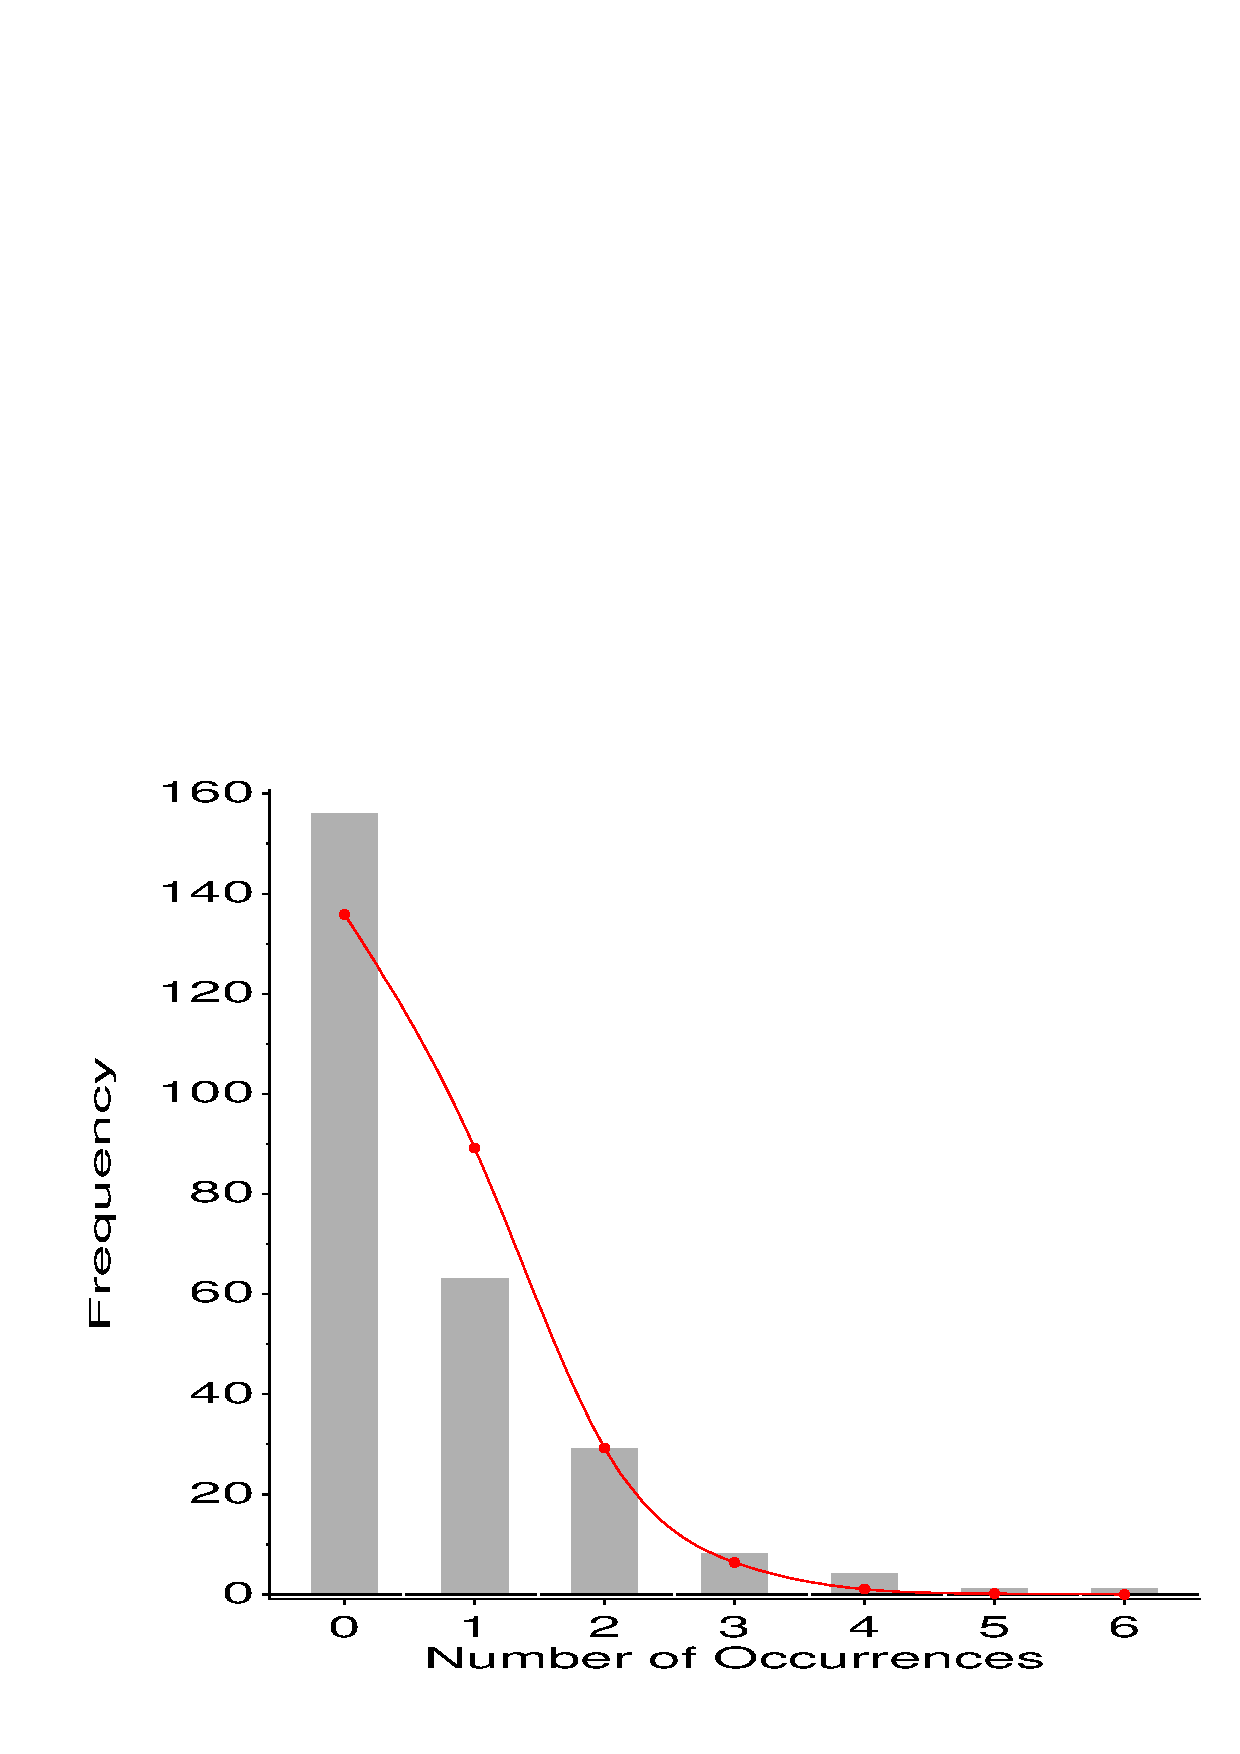
\includegraphics{madfit1}\graphicsfile{ch2/fig/madfit1.eps}{}
 }
 \subfigure[Rootogram]{\label{fig:madfit2}%
  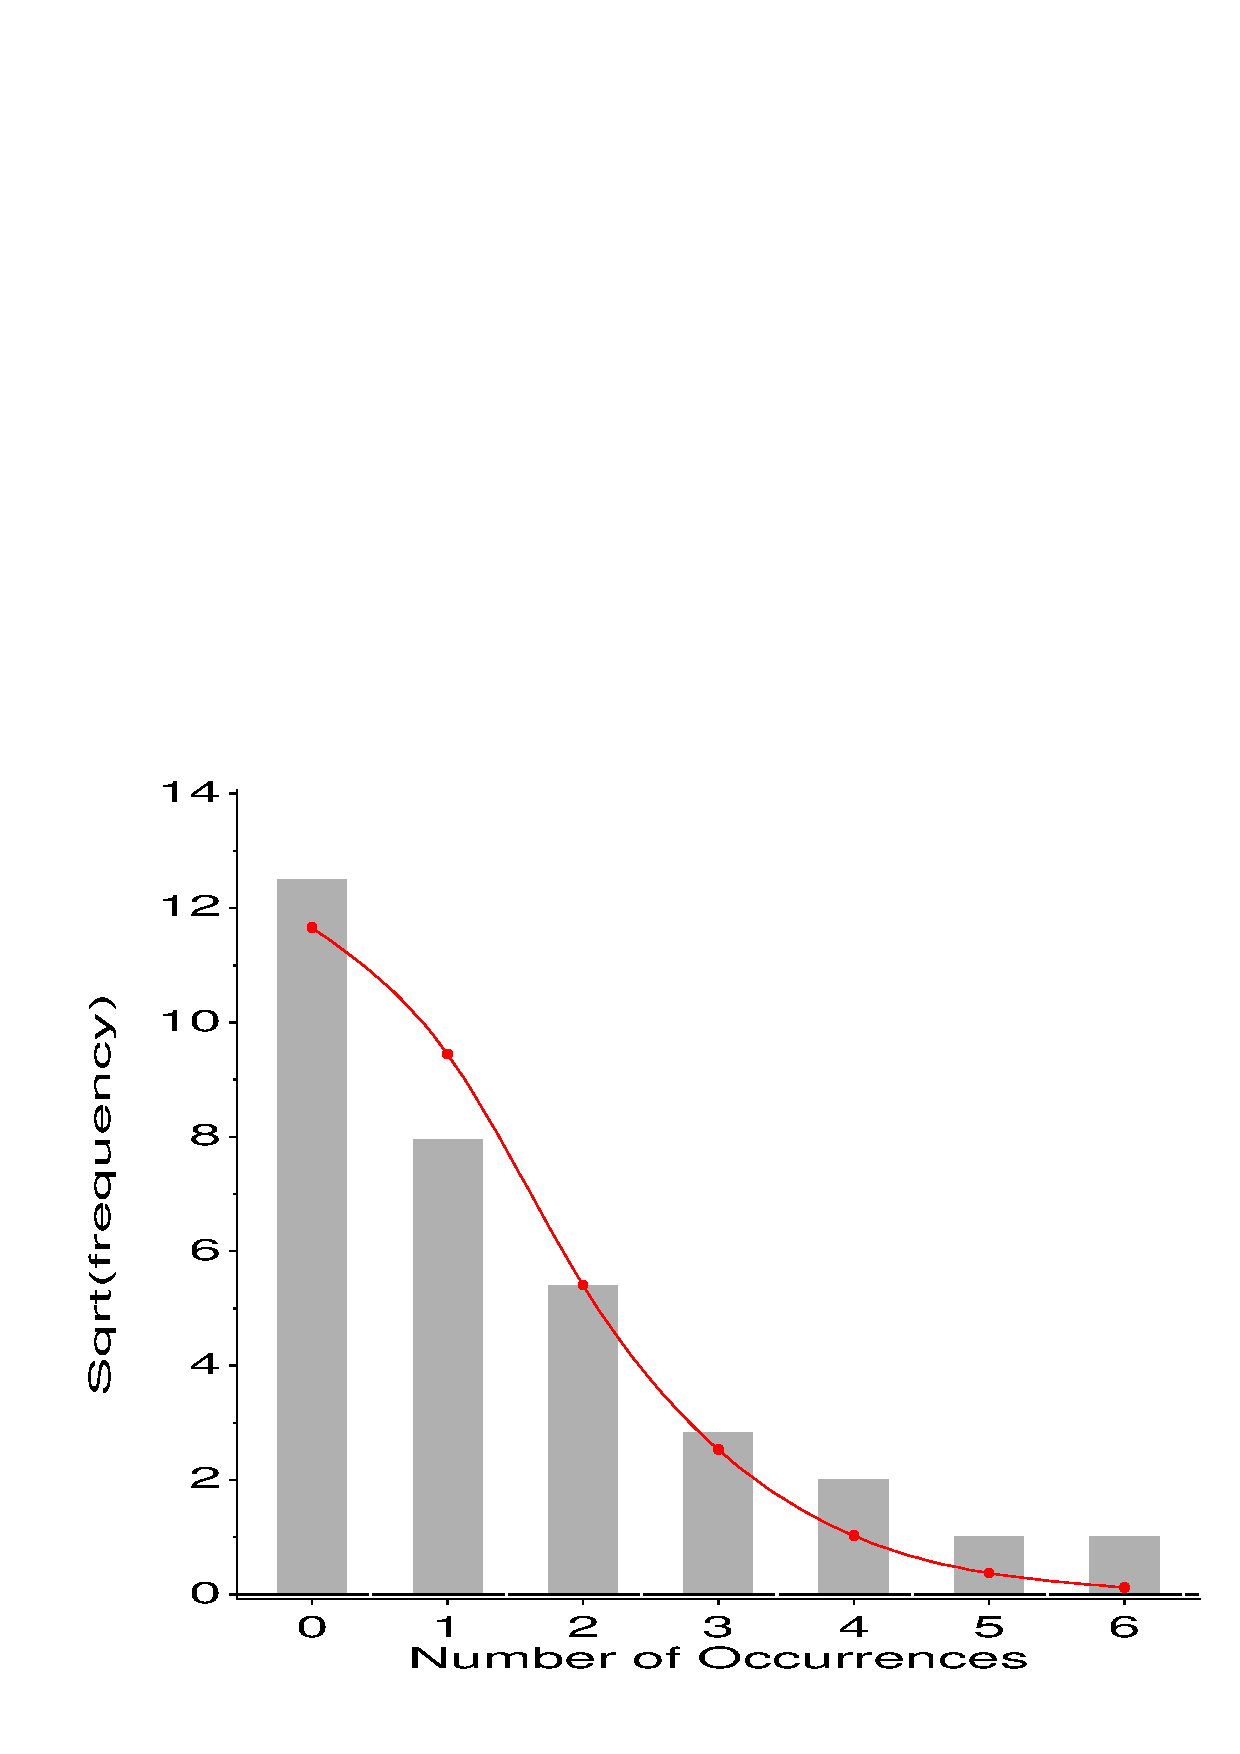
\includegraphics{madfit2}\graphicsfile{ch2/fig/madfit2.eps}{}
 }
 \subfigure[Hanging rootogram]{\label{fig:madfit3}%
  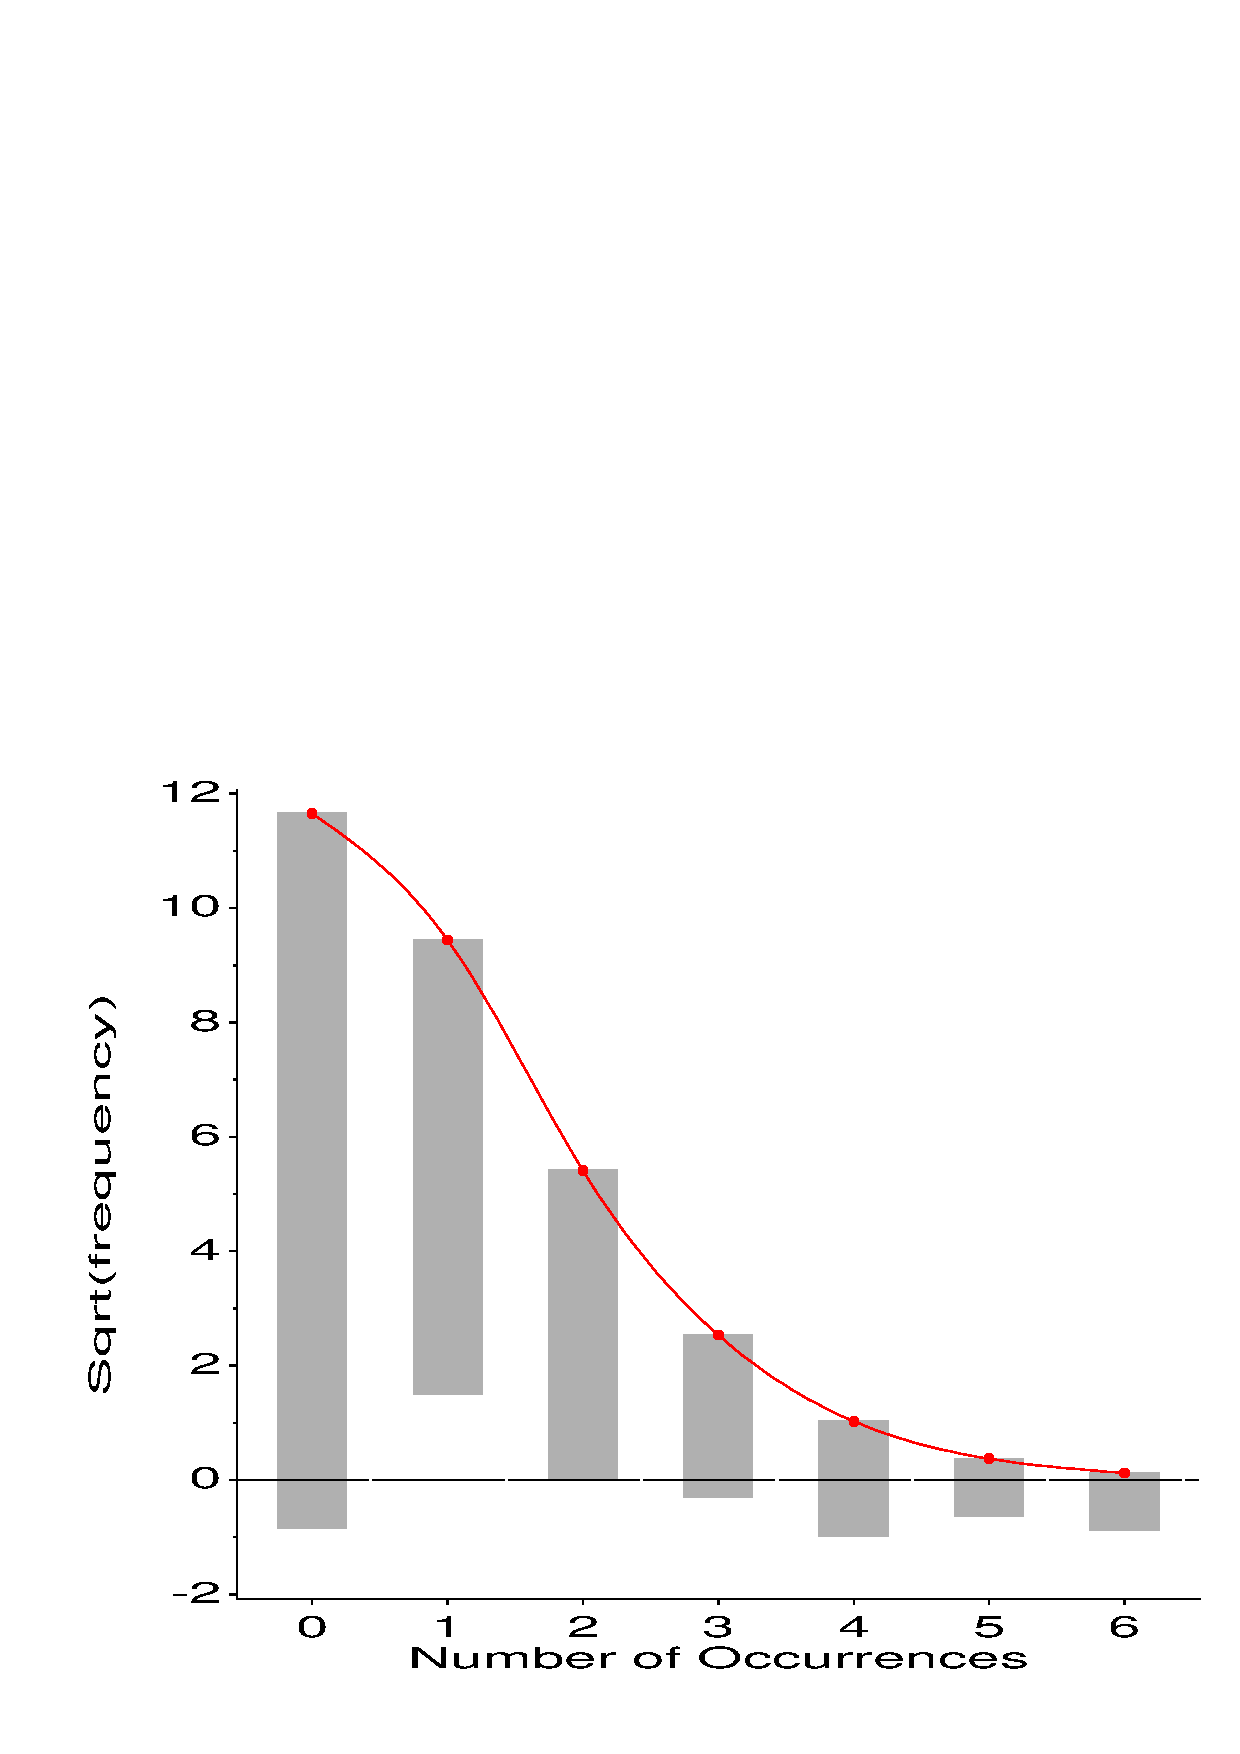
\includegraphics{madfit3}\graphicsfile{ch2/fig/madfit3.eps}{}
 }
 \subfigure[Deviation rootogram]{\label{fig:madfit4}%
  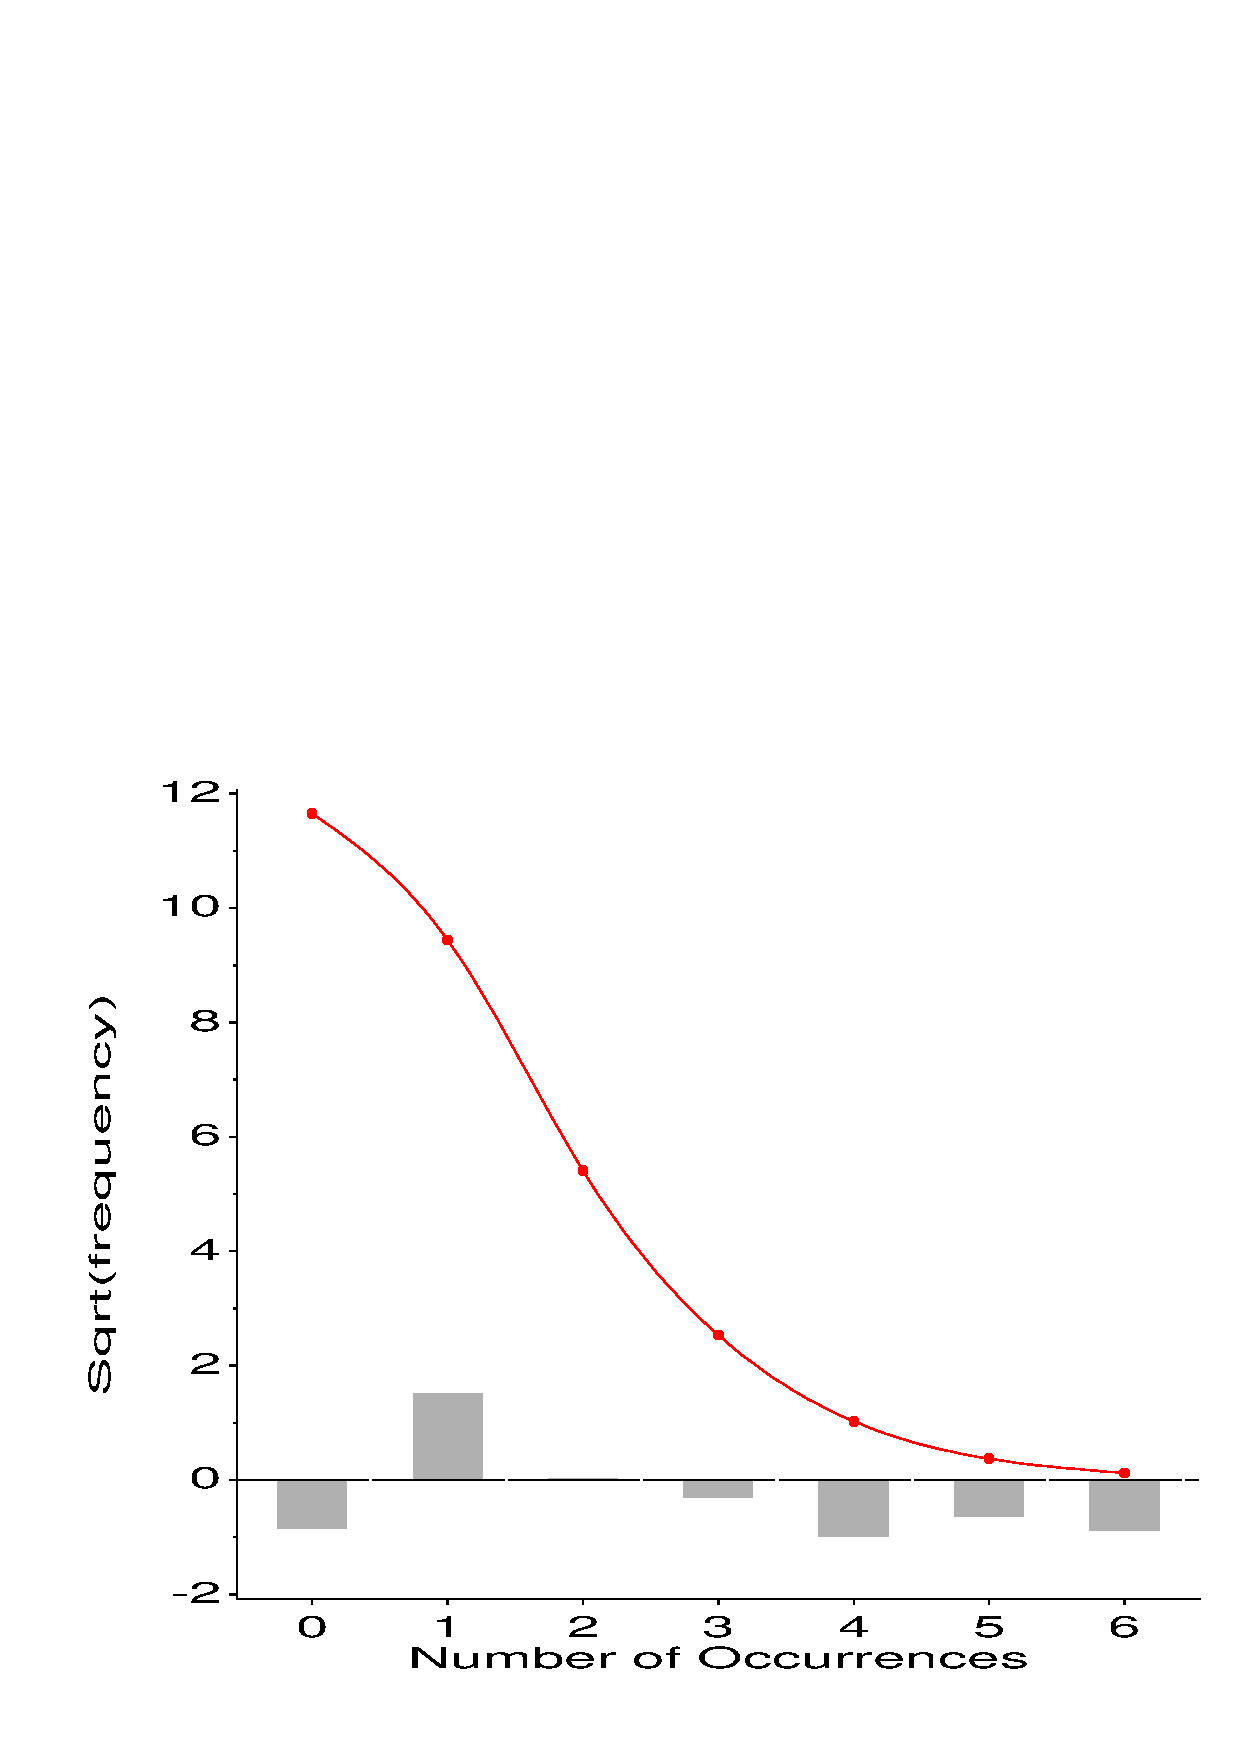
\includegraphics{madfit4}\graphicsfile{ch2/fig/madfit4.eps}{}
 }
 \end{subfigmatrix}
 \caption[Plots of observed and fitted frequencies]{Plots of observed and fitted frequencies
 for the Federalist Papers data, Poisson model.  Each panel shows the fitted frequencies as a smooth
 curve and observed frequencies as a bar.  Panel (a) raw frequencies;
 panels (b)-(d) on a square-root scale, to emphasize smaller frequencies.  Panel (c) is a hanging rootogram, where observed - fitted differences can be judged relative to the horizontal line. Panel (d) shows only the difference between the observed and fi

tted frequency.}\label{fig:madfit}
\end{figure}


\subsection{The \macro{ROOTGRAM}}\label{discrete-root}
The \macro{ROOTGRAM} (\macref{mac:rootgram}) displays observed and fitted frequencies
for a \Dset\ in any of the forms shown in \figref{fig:madfit}.
The input \Dset\ is usually of the form of the output
\texttt{OUT=} \Dset\ produced by the \macro{GOODFIT}.

\begin{Example}[federalist2]{Federalist papers}
We have seen that the negative binomial produces a better fit to the
Federalist Papers data.  The hanging rootogram (\figref{fig:madfit5}),
produced by the statements below, is characteristic of a decent fit.
\begin{listing}
%include catdata(madison);
%goodfit(data=madison, var=count, freq=blocks, dist=negbin, out=fit2);
%rootgram(data=fit2, var=count, obs=blocks, btype=dev);
\end{listing}
%\begin{figure}
%\fig{madfit5.eps}{scale=.7}{madfit5}{Hanging rootogram for the Federalist Papers data, Negative binomial model}
\fig{madfit5}{scale=.7}{Hanging rootogram for the Federalist Papers data, Negative binomial model}
%\end{figure}
\end{Example}


\begin{Example}[saxony1]{Families in Saxony}
Geissler
(cited in \citet{SokalRholf:69}
and \citet{Lindsey:95})
tabulated a huge \Dset\ on sex distributions in families in Saxony
in the 19th century.  Included were $N=6115$ families with $n=12$ children,
which might reasonably be expected to follow a Bin(12,$p$) distribution.
The data are input and fit as shown below.
\input{ch2/sas/saxony}

The fitted distribution, using the estimated proportion of males,
$p = .5192$ is shown in \outref{out:saxony.1};
the goodness of fit tests shown in \outref{out:saxony.2}
indicate that the fit of the Binomial is not good.
The hanging rootogram in \figref{fig:saxony} shows why---%
there is a systematic pattern of deviations from the Binomial,
which produces fitted frequencies too high in the middle and too small
in the tails.
The lack of fit might be ascribed to violations of the assumptions---%
a constant probability of a male birth over a long time span
is a good possibility.
\footnote{\citet[p. 131]{Lindsey:95}
fits a double binomial model with one extra parameter,
and achieves a much better fit, but this too
shows significant lack of fit, not surprising considering the
enormous sample size.}
\begin{Output}
\caption{Fit of the Binomial($12, p$) to the Families in Saxony data: Observed and fitted frequencies}\label{out:saxony.1}
\small
\verbatiminput{ch2/out/saxony.1}
\end{Output}
\begin{Output}
\caption{Fit of the Binomial($12, p$) to the Families in Saxiony data: Goodness of fit tests}\label{out:saxony.2}
\small
\verbatiminput{ch2/out/saxony.2}
\end{Output}

\begin{figure}[htb]
  \centering
  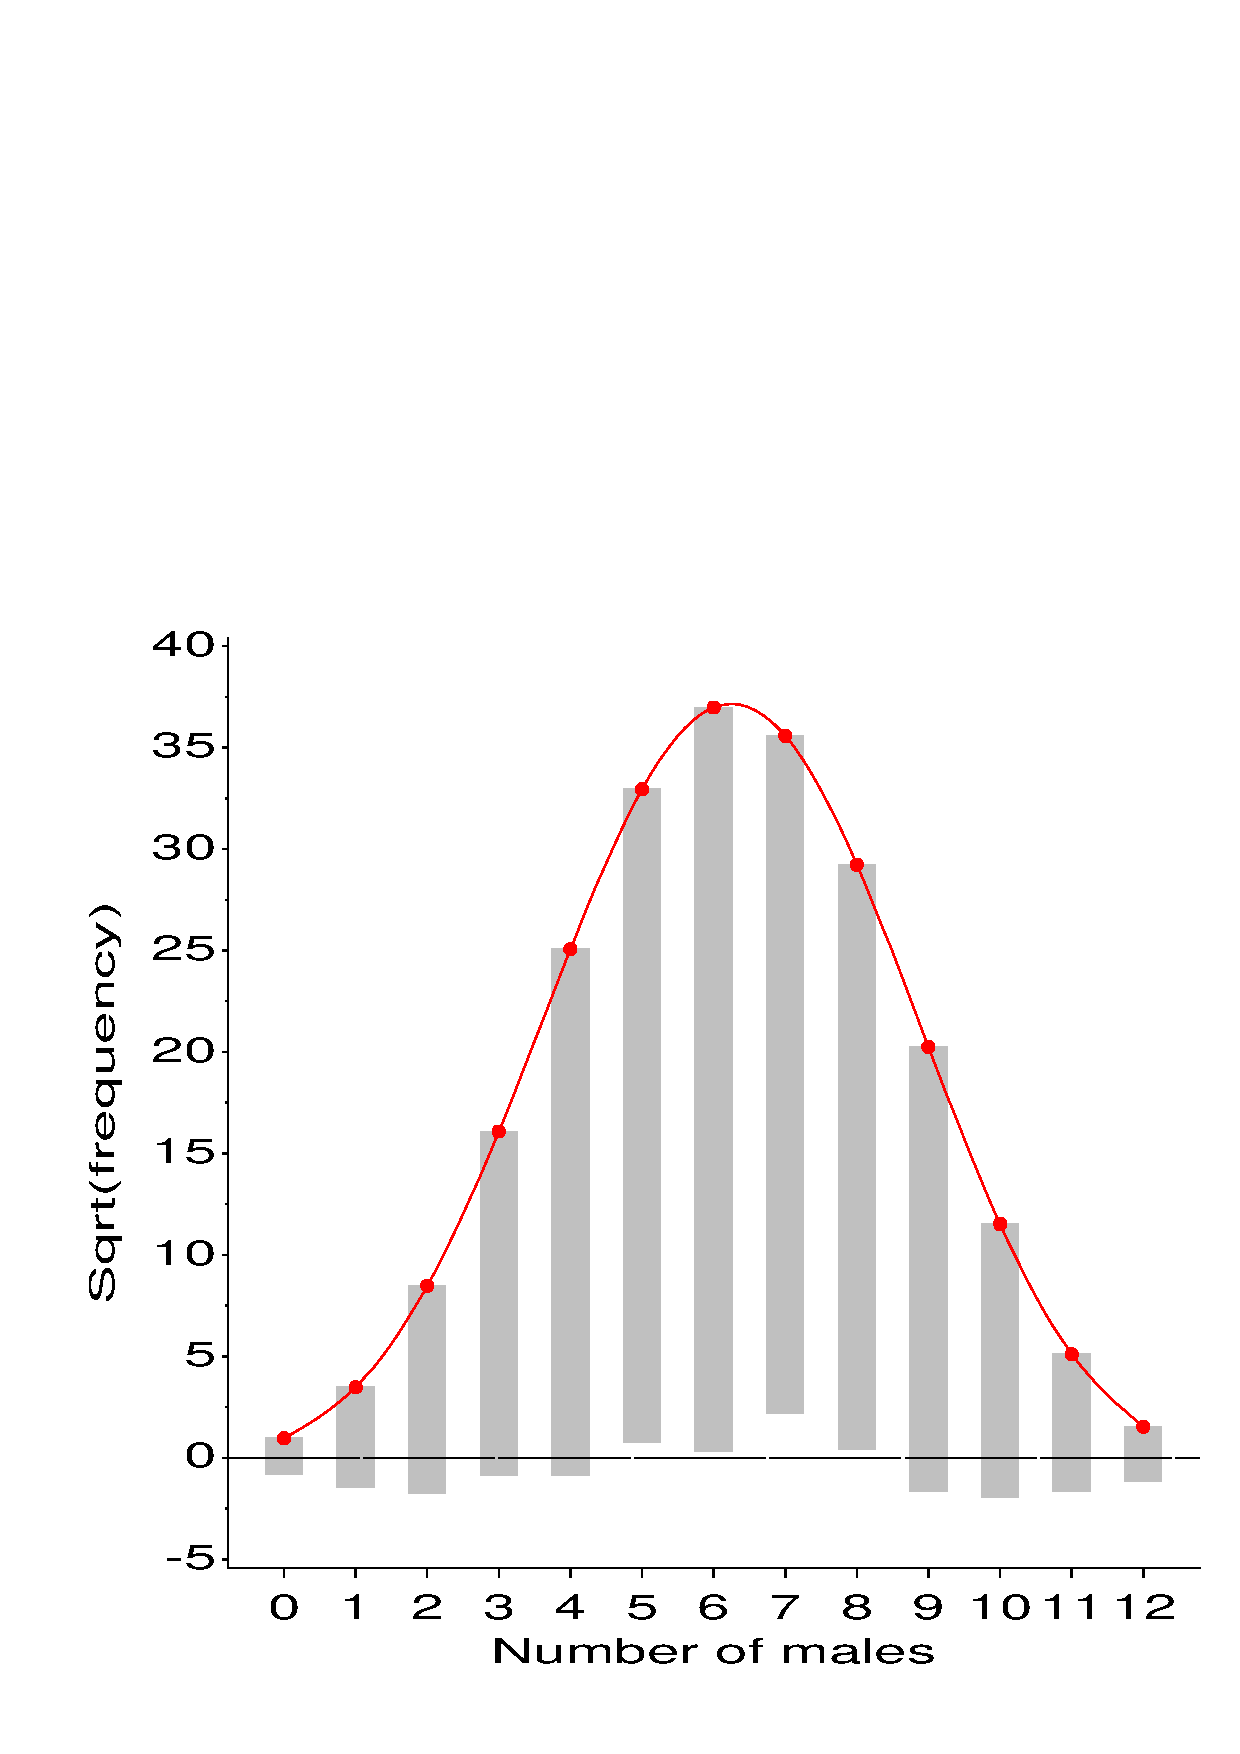
\includegraphics[scale=.5]{saxony}\graphicsfile{ch2/fig/saxony.eps}{}
  \caption[Hanging rootogram for Saxony families, Binomial model]{Hanging rootogram for Saxony families, Binomial($12, p$) model.
The systematic pattern of deviations shows that the Binomial model is not completely adequate for these data.}\label{fig:saxony}
\end{figure}
\end{Example}


\subsection{Maximum likelihood estimation}
\secref{sec:discrete-distrib} described the common discrete distributions,
their probability functions, and sample estimates.
Here we consider the general case.
Suppose we have a multinomial sample of
$K$ ``groups'', with frequencies of $n_k$ in group
$k$, and $\sum_k n_k = N$.
Suppose further that we have a probability model which specifies
the probability, \( \pi_k (\vec{\theta}), \: k = 1, 2, \dots ,  K \),
of an observation in group $k$, where $\vec{\theta}$ is a vector
of $s \geq 0$ parameters of the distribution
and $\sum_k \pi_k (\vec{\theta}) = 1$.

The likelihood, $\mathcal{L}$, is the probability of the data as
a function of the parameters,

\begin{equation*}
  \mathcal{L}(\vec{\theta}) = n ! \prod_{k=1}^K \frac{\pi_k (\vec{\theta})^{n_k}}{n_k !}
\end{equation*}

We can determine the value(s) of $\vec{\theta}$ which maximize $\mathcal{L}$
by maximizing the log-likelihood,

\begin{equation}\label{eq:loglikelihood}
 \ell(\vec{\theta}) \equiv
 \log \mathcal{L}(\vec{\theta}) = \log n ! +
  \sum_{k=1}^K n_k \log \pi_k (\vec{\theta}) - \sum_{k=1}^K \log n_k !
\end{equation}
The maximum likelihood estimate (MLE) of $\vec{\theta}$ will be
the value $\hat{\vec{\theta}}$ which is the solution of the
estimating equations
\begin{equation*}
\frac{\partial \log \mathcal{L}(\vec{\theta})}{\partial \vec{\theta}_i} = 0
\quad\quad i=1, 2, \dots s
\end{equation*}

For example, for the geometric distribution with probability
function \eqref{eq:geomf}, the log-likelihood is
\begin{equation*}
 \ell(\vec{\theta})   = n \log \theta +
  \sum_{k=1}^K (n_k - 1) \log (1-\theta)
\end{equation*}
which gives the estimating equation,
\begin{equation*}
\frac{\partial \ell(\theta)}{\partial \theta} =
\frac{(\sum_k n_k) - n}{1-\theta} + \frac{n}{\theta} = 0
\end{equation*}
whose solution is $\hat{\theta} = 1/\bar{k}$.  The fitted probabilities
under the geometric model
are then $\pi_k (\hat{\theta}) = (1 - \hat{\theta})^{k-1} \hat{\theta}$.

Having found the maximum likelihood estimate of the parameters, the
likelihood ratio
goodness-of-fit \GSQ{} statistic compares the maximized value of the
log-likelihood to the maximized log-likelihood of an unrestricted model
where the probabilities are only constrained so that $\sum_k \pi_k =1$.
In this case, there are $s=0$ parameters, and we symbolize the log-likelihood
by $ \ell(\theta_0) \equiv \ell(\vec{\pi})$.  For a multinomial sample this is

\begin{equation}\label{eq:loglikelihood0}
 \ell(\vec{\theta}_0)  = \log n ! +
  \sum_{k=1}^K n_k \log \pi_k  - \sum_{k=1}^K \log n_k !
\end{equation}
Maximizing \eqref{eq:loglikelihood0} subject to $\sum_k \pi_k =1$
gives $\hat{\pi}_k = n_k / N$.
The likelihood ratio statistic is

\begin{equation}\label{eq:likeratio}
 G^2 = -2 \log \left[
 \frac{\mathcal{L}(\vec{\theta}_0)}{\mathcal{L}(\vec{\theta})}
 \right]
 = 2 [ \ell(\vec{\theta}) - \ell(\vec{\theta}_0) ]
 = 2 \sum_{k=1}^{K} n_k \log \left( \frac{n_k}{N \pi_k (\hat{\theta}) } \right)
\end{equation}
which follows an asymptotic chi-square distribution with $K-1-s$ degrees
of freedom.


\subsection{Fitting discrete distributions as \loglin\ models}
In \secref{sec:pwrseries}, I described how the common discrete distributions
are all members of the general power series family.
Another general family of distributions---the exponential family---%
includes most of the common continuous distributions:
the normal, gamma, exponential, and others,
and is the basis of the class of generalized linear models fit
by \PROC{GENMOD}.

\citet{LindseyMersch:92}, \citet[6.1]{Lindsey:95} have shown how various discrete
(and continuous)
distributions can be fit to frequency data using Poisson \loglin{} models
available in \PROC{GENMOD}.  The uniform, geometric, binomial, and the
Poisson distributions may all be fit easily in this way.
A clear advantage is that this method gives estimated standard errors for the
distribution parameters as well as estimated confidence intervals
for fitted probabilities.

The essential idea is that, for frequency data, any distribution in the
exponential family may be represented by a linear model for the logarithm
of the cell frequency, with a Poisson distribution for errors,
otherwise known as a ``Poisson \loglin\ regression model''.
These have the form
\begin{equation*}
\log (N \pi_k) = \textrm{ offset } + \beta_0 + \vec{\beta}\trans \vec{S}(k)
 \comma
\end{equation*}
where $\vec{S}(k)$ is a vector of zero or more sufficient statistics for the
canonical parameters of the exponential family distribution,
and the offset term is a value which does not depend on the
parameters.  \tabref{tab:expfamily} shows the sufficient statistics and
offsets for several discrete distributions.
See \citet{LindseyMersch:92} for further details, and definitions
for the double-binomial distribution.

\input{ch2/tab/expfamily}

\begin{Example}[saxony2]{Families in Saxony}
The binomial distribution and the double binomial can both be fit to frequency data as a Poisson
regression using $\log \binom{n}{k}$ as an offset.
We only display results for the binomial model.
\begin{listing}
*-- calculate offset variables for binomial and double binomial;
data saxony;
   set saxony;
   logkn = log( gamma(12+1) / (gamma(males+1) * gamma(12-males+1)) );
   if 0 < males < 12
      then ylogity = -males * log(males/(12-males));
      else ylogity = 0;

   *-- fit binomial (12,p);
proc genmod data=saxony;
   model families = males /
      dist=poisson offset=logkn obstats ;

   *-- fit double binomial (12,p, psi);
proc genmod data=saxony;
   model families = males ylogity /
      dist=poisson offset=logkn obstats ;
\end{listing}
The goodness of fit tests shown in \outref{out:saxony2.1}
are equivalent to those calculated directly by the
\macro{GOODFIT} in \outref{out:saxony.2}.
The parameter estimate for \texttt{MALES}, $\beta_1 = 0.0769$
is actually estimating the logit of $p$, $\log p / (1-p)$,
so the inverse transformation gives
$\hat{p} = \frac{\exp (\beta_1)}{1 + \exp (\beta_1)} = 0.5192$,
as we had before.
The fitted frequencies (shown in \outref{out:saxony2.2}), given by the \opt{OBSTATS}{GENMOD}
on the \stmt{MODEL}{GENMOD} are the same as those
in \outref{out:saxony.1}.
The standard error for \texttt{MALES}, $s_{\beta_1} = 0.0074$
could also be transformed back to the probability scale in the same
way.
\begin{Output}
\caption{Fit of the Binomial($12, p$) to the Families in Saxony data: Goodness of fit tests}\label{out:saxony2.1}
\small
\verbatiminput{ch2/out/saxony2.1}
\end{Output}
\begin{Output}
\caption{Fit of the Binomial($12, p$) to the Families in Saxony data: Observed and fitted frequencies}\label{out:saxony2.2}
\small
\verbatiminput{ch2/out/saxony2.2}
\end{Output}
\end{Example}



\section{Diagnosing discrete distributions: Ord plots}%
\label{sec:discrete-Ord}
\ix{Ord plot|(}
Ideally, the general form chosen for a discrete distribution should
be dictated by substantive knowledge of a plausible mechanism
for generating the data.
When such knowledge is lacking, however,
we may not know which distribution is most appropriate for
some particular set of data.
In these cases, the question is often turned around, so that we seek
a distribution that fits well, and then try to understand the mechanism
in terms of aspects of the underlying probability theory (independent trials,
rare events, waiting-time to an occurrence, and so forth).

Although it is possible to fit each of several possibilities,
the summary goodness-of-fit statistics can easily be influenced by
one or two disparate cells, or additional (ignored or unknown) factors.
One simple alternative is a plot suggested by
\citet{Ord:67} which may be used to diagnose
the form of the discrete distribution.  Ord showed that a linear
relationship of the form,
\begin{equation} \label{eq:ord}
  \frac{ k \,  p(k) } { p(k-1) }
 = a  +  b \,  k \comma
\end{equation}
holds for each of the Poisson, binomial, negative binomial, and
logarithmic series distributions, and these distributions are
distinguished by the signs of the intercept,
$a$, and slope, $b$, as shown in
\tabref{tab:ordparm}.
The slope, \(b\),
in \eqref{eq:ord} is zero for the
Poisson, negative for the binomial, and positive for the negative
binomial and logarithmic series distributions; the latter two are
distinguished by their intercepts.
\ix{Poisson distribution}
\ix{logarithmic series distribution}
\ix{binomial distribution}
\ix{negative binomial distribution}

Thus, a plot of \(k \,  n_k /  n_{k-1}\) against \(k\), if linear,
is suggested as a means to determine which of these distributions to apply.
The values of the slope and intercept provide rough estimates of the
distribution parameters.

\begin{table}[htb]
\caption[Diagnostic slope and intercept for four discrete distributions]{Diagnostic slope and
intercept for four discrete distributions.  The ratios $k n_k / n_{k-1}$ plotted
against $k$ should appear as a straight line, whose slope and intercept
determine the particular distribution.}
\label{tab:ordparm}
\begin{center}
%\vspace{1ex}
\begin{tabular}{|ccll|}\hline
Slope & Intercept & Distribution & Parameter \\
(b)   & (a)       & (parameter)  &  estimate \\ \hline
0     &  $+$      &  Poisson (\(\lambda\)) & \(\lambda = a\)    \\
$-$   &  $+$      &  Binomial (n, p)       & \(p = b / (b-1)\)  \\
$+$   &  $+$      &  Negative binomial (n,p)      & \(p = 1 - b\)      \\
$+$   &  $-$      &  Log.\ series (\(\theta\)) & \(\theta =  b\) \\
      &      &                     &   \(\theta = - a\) \\ \hline
\end{tabular}
\end{center}
\end{table}

\subsubsection{Fitting the line}
One difficulty in applying this technique is that the number of points
(distinct values of $k$)
in the Ord plot is often small, and the sampling variances of
\(k \,  n_k /  n_{k-1}\) can vary enormously.
A little reflection indicates that points where $n_k$ is small
should be given less weight in determining the slope of the
line (and hence determining the form of the distribution).
In the small number of cases I've
tried, I have found that using a weighted least squares fit of \(k \,
n_k /  n_{k-1}\) on \(k\), using weights of \(w_k = \sqrt { n_k -1
}\)
produces reasonably good%
\footnote{This definition implies that frequencies of $n_k =1$
are ignored in fitting the line.}
automatic diagnosis of the form of a
probability distribution, but this choice is surely open to further study.

\subsubsection{Examples}
\begin{Example}[horskick3]{Death by horse kick}
The table below shows the calculations for
the horse kicks data, with the ratio \({ k \,  n_k } /  { n_{k-1}
}\) labeled \texttt{y}.  The weighted least squares line, with weights
\(w_k\), has a slope close to zero, indicating the Poisson
distribution.  The estimate \(\lambda = a = .656\) compares
favorably with the MLE, $\lambda=0.610$ and the
value from the Poissonness plot, shown in the
following section.
\ixd{death by horse kick}

\begin{alltt}
      Ord Plot: Deaths by Horsekicks

   k     \(n\sb{k}\)    \(n\sb{k-1}\)       \(w\sb{k}\)         y

   0    109      .    10.3923     .        -- Weighted LS --
   1     65    109     8.0000    0.5963    slope = -0.034
   2     22     65     4.5826    0.6769    inter = 0.656
   3      3     22     1.4142    0.4091
   4      1      3     0.0000    1.3333
\end{alltt}
\end{Example}

\begin{Example}[madison3]{Federalist papers}
For the word frequency data, the slope is positive, so either the
negative binomial or log series are possible.  The intercept is
essentially zero, which is ambiguous.  However, the logarithmic
series requires \(b \approx  - a\), so the negative binomial is a
better choice.  Mosteller \& Wallace did in fact find a reasonably
good fit to this distribution.
\ix{logarithmic series distribution}
\ix{negative binomial distribution}
\ixd{Federalist papers}

\begin{alltt}
      Instances of 'may' in Federalist papers

   k     \(n\sb{k}\)    \(n\sb{k-1}\)       \(w\sb{k}\)         y

   0    156      .    12.4499     .       -- Weighted LS --
   1     63    156     7.8740    0.4038   slope = 0.424
   2     29     63     5.2915    0.9206   inter = -0.023
   3      8     29     2.6458    0.8276
   4      4      8     1.7321    2.0000
   5      1      4     0.0000    1.2500
   6      1      1     0.0000    6.0000
\end{alltt}

Plots of data fitting four different discrete distributions are
shown in \figref{fig:orddemo}, using the data previously examined
in this chapter.
In each case, the slope and intercept of the weighted least squares line correctly
identify the distribution.
\end{Example}

\subsubsection{Drawbacks}
Using a single plot to determine one of four common discrete
distributions is advantageous, but our enthusiasm should be
limited by several weaknesses:

\begin{itemize*}
\item The Ord plot lacks resistance, since a single discrepant
       frequency affects the points for both \(k\) and \(k  +  1\).

\item The sampling variance of \(k \,  n_k /  n_{k-1}\) fluctuates
       widely
       \citep{HoaglinTukey:85,JinkinsonSlater:81}.  The use of weights \(w_k\) helps, but is purely a
       heuristic device.
\end{itemize*}


\begin{figure}[htb]
 \begin{minipage}[b]{.5\linewidth}
  \centering
  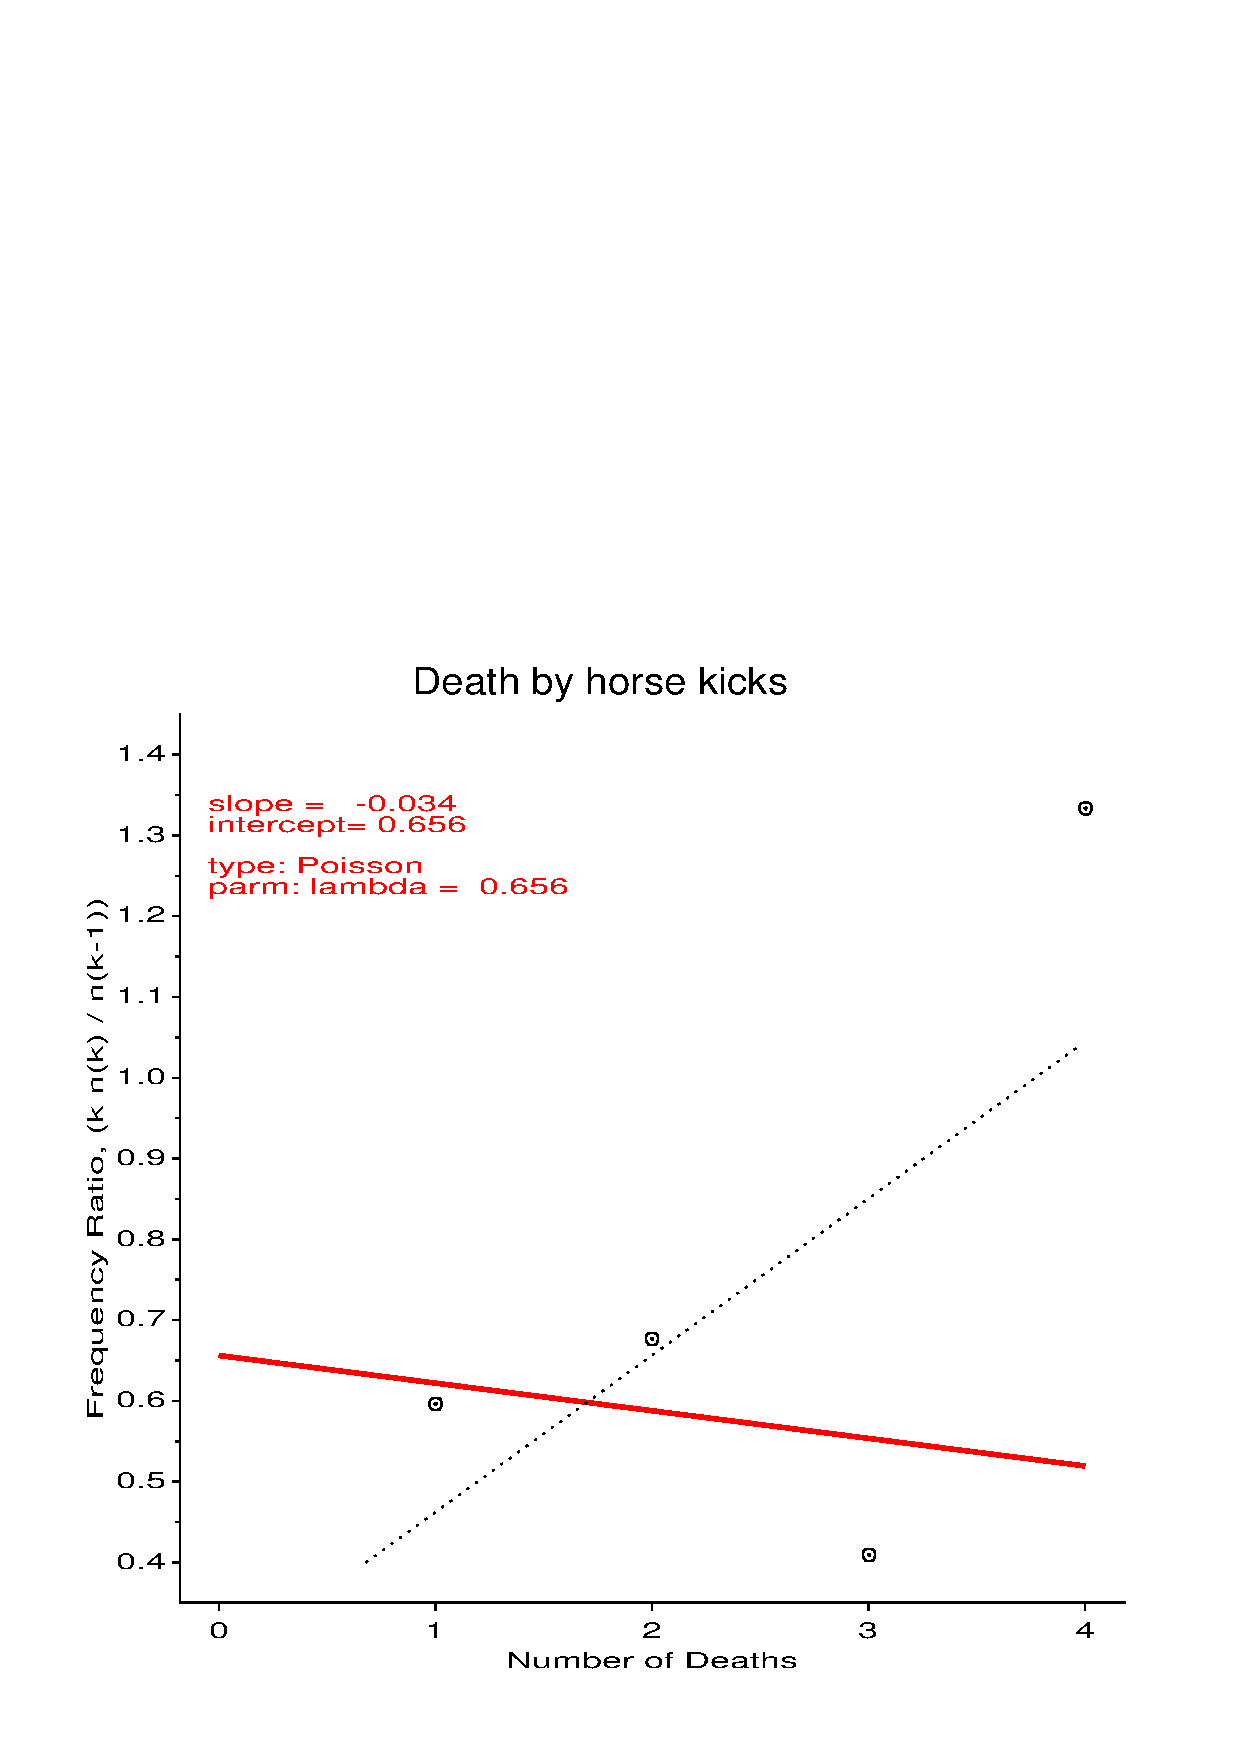
\includegraphics[width=.9\linewidth]{orddemo1}\graphicsfile{ch2/fig/orddemo1.eps}{}
 \end{minipage}%
 \begin{minipage}[b]{.5\linewidth}
  \centering
  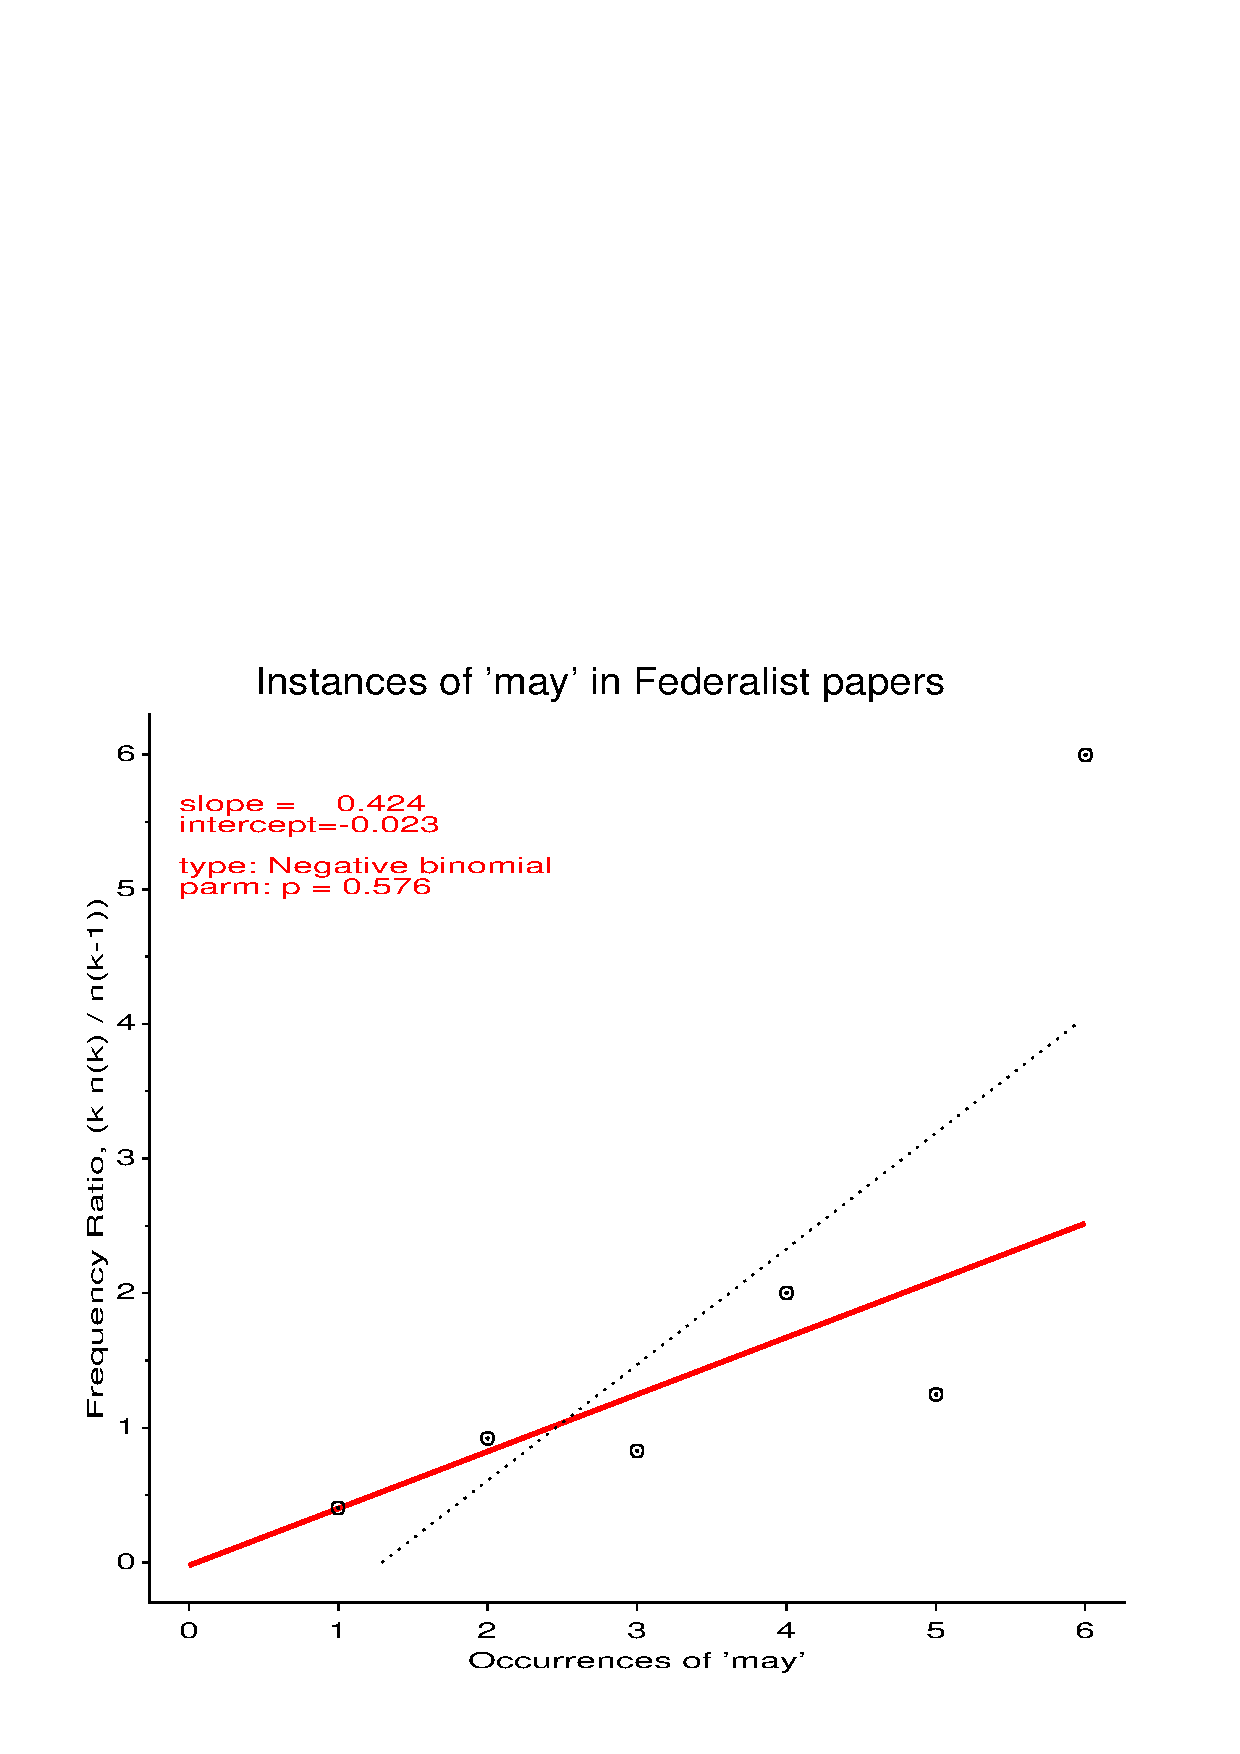
\includegraphics[width=.9\linewidth]{orddemo2}\graphicsfile{ch2/fig/orddemo2.eps}{}
 \end{minipage}
 \\[3ex]
 \begin{minipage}[b]{.5\linewidth}
  \centering
  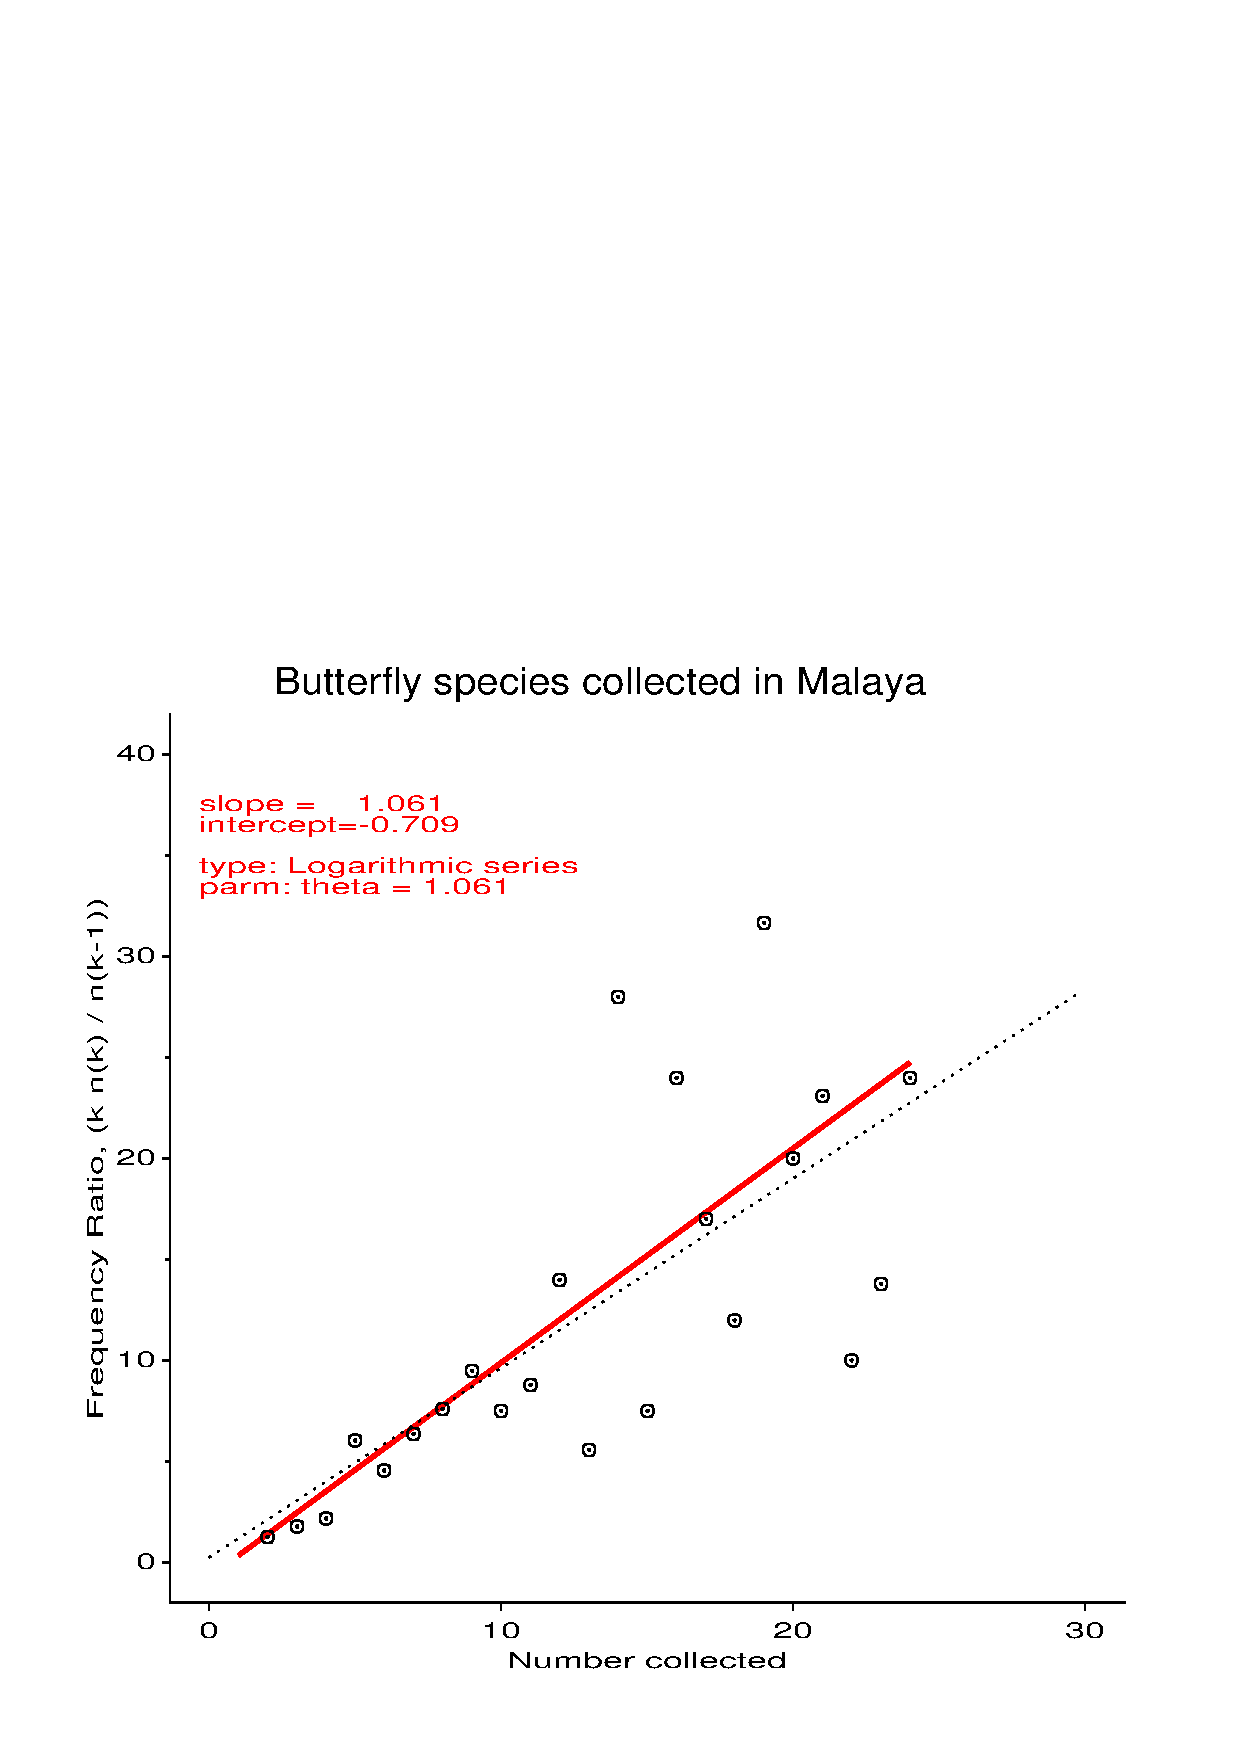
\includegraphics[width=.9\linewidth]{orddemo3}\graphicsfile{ch2/fig/orddemo3.eps}{}
 \end{minipage}%
 \begin{minipage}[b]{.5\linewidth}
  \centering
  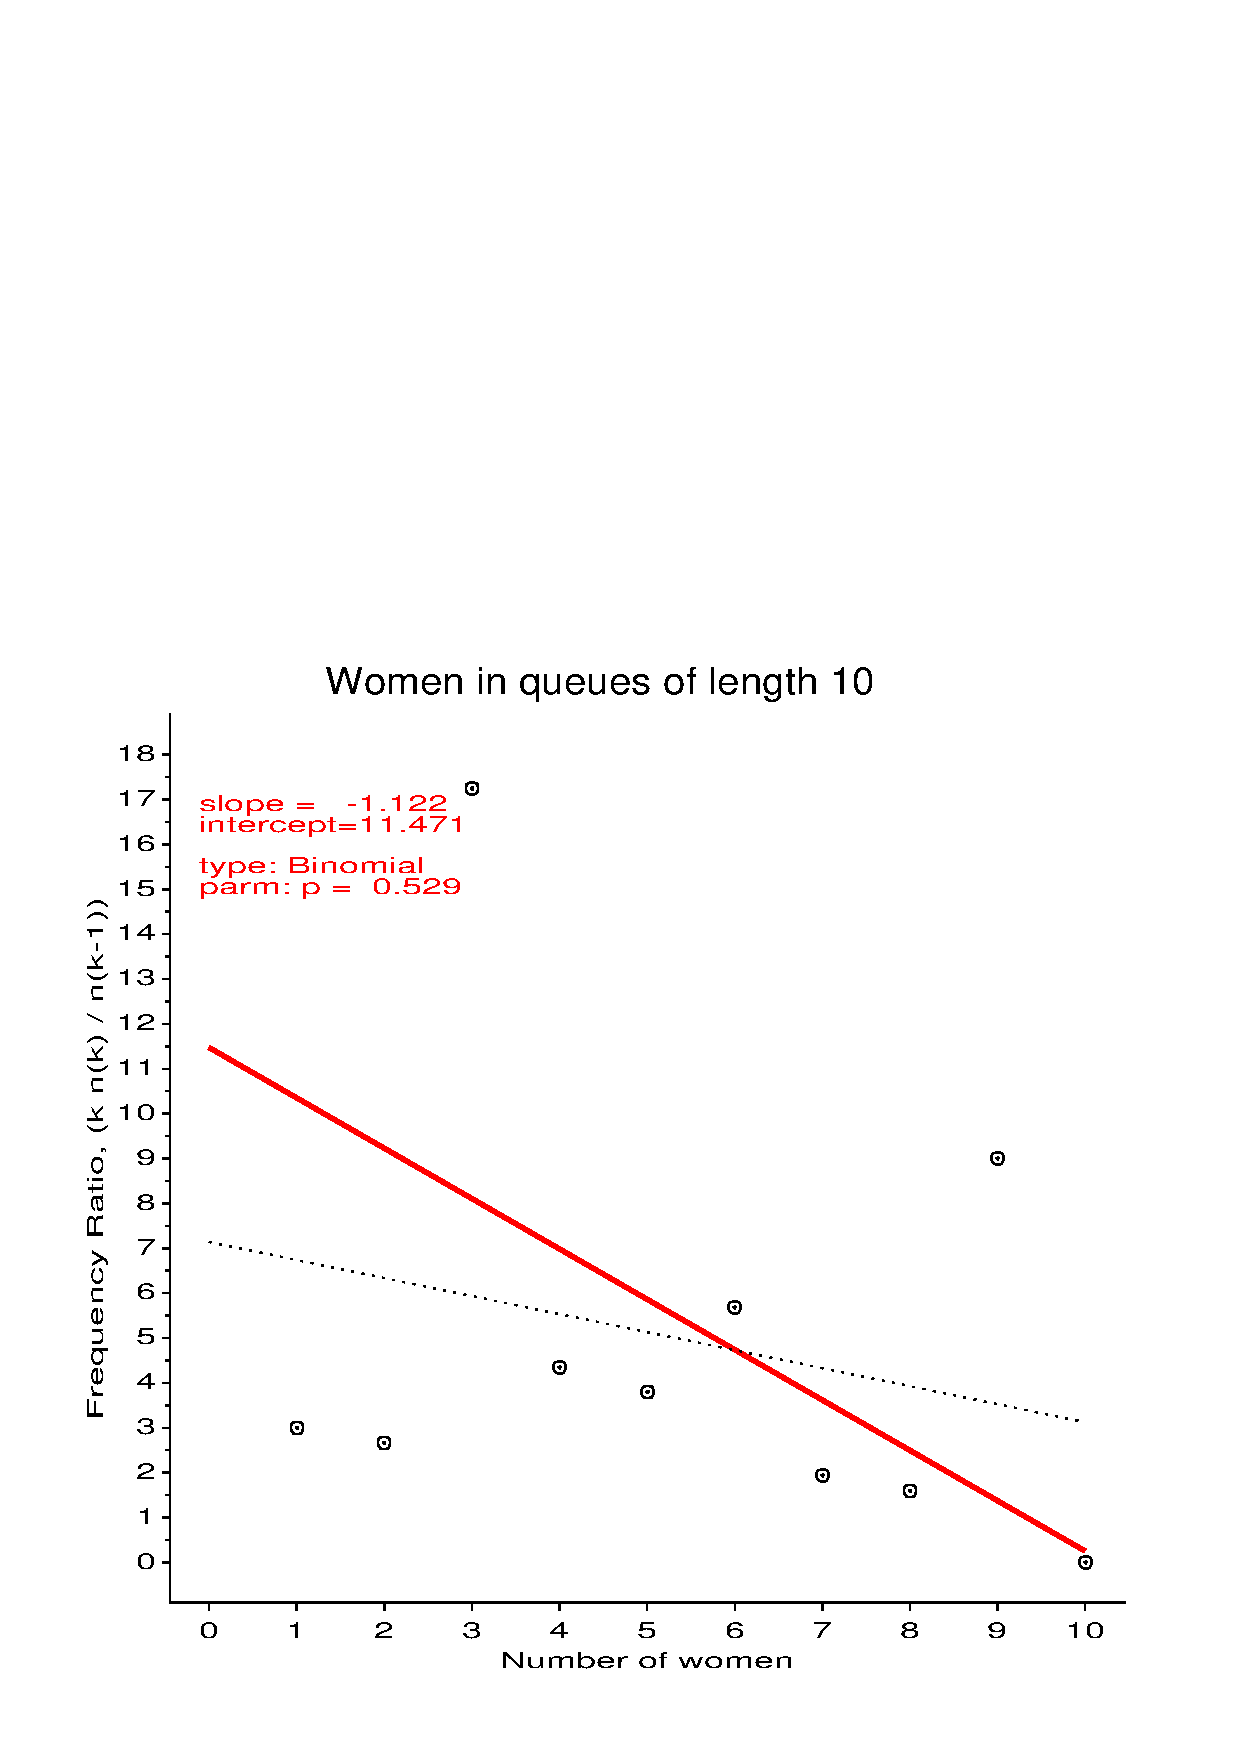
\includegraphics[width=.9\linewidth]{orddemo4}\graphicsfile{ch2/fig/orddemo4.eps}{}
 \end{minipage}
 \caption[Ord plots for four discrete distributions]{Ord plots for four discrete
distributions.  Each panel shows the least squares line (dotted, black) and the weighted least squares line (solid, red). The slope and intercept of the weighted least squares line are used to
identify the type of the distribution.}\label{fig:orddemo}
\end{figure}

\subsubsection{ORDPLOT macro}
These plots are produced by the \macro{ORDPLOT} (see \ref{mac:ordplot}).  For the horse kicks
data,  the plot in \figref{fig:orddemo} is produced with the macro call
\begin{listing}
%ordplot(data=horskick,
         count=Deaths, freq=corpsyrs);
\end{listing}
The \mparm{FREQ}{ORDPLOT} gives the name of the basic frequency variable ($k$),
and the \mparm{COUNT}{ORDPLOT} gives the associated count, $n_k$.
\ix{Ord plot|)}

\section{Poissonness plot}\label{sec:discrete-Poissonness}
\ix{Poissonness plot|(}

The Poissonness plot
\citep{Hoaglin:80}
is designed as a plot of some
quantity against \(k\), so that the result will be points along a
straight line when the data follow a \IX{Poisson distribution}.  When the
data deviate from a Poisson, the points will be curved.
\citet{HoaglinTukey:85}
develop similar plots for other discrete distributions,
including the binomial, negative binomial, and logarithmic series
distributions.
\ix{binomial distribution}
\ix{negative binomial distribution}

\subsection{Features of the Poissonness plot}
The Poissonness plot has the following desirable features:
\begin{itemize}
\item \boldital{Resistance}: a single discrepant value of \(n_k\)
       affects only the point at value \(k\).  (In the Ord plot
       it affects each of its neighbors.)
\item \boldital{Comparison standard}:  An approximate confidence
       interval can be found for each point, indicating its inherent
       variability and helping to judge whether each point is
       discrepant.
\item \boldital{Influence}:  Extensions of the method result in
       plots which show the effect of each point on the estimate of
       the main parameter of the distribution (\(\lambda\) in the
       Poisson).
\end{itemize}

\subsection{Plot construction}
Assume, for some fixed \(\lambda\), each observed frequency, \(n_k\)
equals the expected frequency, \(m_k = N p_k\).  Then, setting
\(n_k = N p_k  = N { e^{ - \lambda } \:  \lambda^k } /  { k ! }\),
and taking logs of both sides gives

\begin{equation*}
  \log ( n_k ) = \log \,  N - \lambda  +  k \,  \log \,  \lambda  -
  \log \,  k !
\end{equation*}
which can be rearranged to
\begin{equation} \label{eq:poispl}
  \log \left(  \frac{ k ! \:  n_k } {N} \right)
 = - \lambda  +  ( \log \,  \lambda ) \,  k
 \period
\end{equation}

The left side of \eqref{eq:poispl} is called the \glossterm{count metameter}, and
denoted \(\phi \,  ( n_k )  = \log_e ( k ! \,  n_k  /  N )\).  Hence,
plotting \(\phi ( n_k )\) against \(k\) should give a line
\(\phi ( n_k )= a + b k\) with

\begin{itemize*}
\item slope = \(\log  \,  \lambda\)
\item intercept = \(- \lambda\)
\end{itemize*}
when the observed frequencies follow a Poisson distribution.
If the points in this plot are close enough to a straight line,
then an estimate of $\lambda$ may be obtained from the slope $b$ of the line,
$\hat{\lambda} = e^b$ should be reasonably close in value
to the MLE of $\lambda$, $\hat{\lambda} = \bar{x}$.
In this case, we might as well use the MLE as our estimate.

\subsubsection{Leveled plot}
If we have a preliminary estimate $\lambda_0$ of $\lambda$,
we can use this to give a new plot where the reference line
is horizontal, making comparison of the points with the line
easier.
In this leveled plot the vertical coordinate $\phi (n_k)$ is modified to
\begin{equation*}
 \phi ' (n_k) = \phi (n_k) + \lambda_0 - k \log \lambda_0
 \period
\end{equation*}
When the data follow a Poisson distribution with parameter
$\lambda$, the modified plot will have
\begin{itemize*}
\item slope = \(\log  \lambda - \log  \lambda_0 = \log ( \lambda / \lambda_0 ) \)
\item intercept = \(\lambda_0 - \lambda\)
\end{itemize*}
In the ideal case, where our estimate of $\lambda_0$ is close to the true
$\lambda$, the line will be horizontal at $\phi ' = 0$.
The modified plot is particularly useful in conjunction with the
confidence intervals for individual points described below.

\subsubsection{Confidence intervals}
When one or two points deviate from an otherwise nearly linear
relation,
it is helpful to determine whether the discrepancy is consistent with
chance variation.
As well, we must recognize that classes with small frequencies $n_k$
are less precise than classes with large frequencies.
\citet{HoaglinTukey:85} develop approximate confidence intervals
for $\log m_k$ for each point in the Poissonness plot.
These are calculated as
\begin{equation*}
\phi \left( n_k^{*}\right) \pm h_k
\end{equation*}
where the count metameter function is calculated using a modified frequency $%
n_k^{*}$, defined as

\begin{equation*}
n_k^{*}= \left\{
\begin{array}{ll}
n_k-.8n_k-.67 & n\geq 2 \\
1/e & n=1 \\
\textrm{undefined} & n=0
\end{array}
\right.
\end{equation*}
%
and $h_k$ is the half-width of the 95\% confidence interval,
\begin{equation*}
h_k=1.96\frac{\sqrt{1-\widehat{p}_k}}{[n_k-(.25\widehat{p}_k+.47)\sqrt{n_k}%
]^{1/2}}
\end{equation*}
and $\hat{p}_k = n_k / N$.

\subsection{The \macro{POISPLOT}}
The \macro{POISPLOT} (see \macref{mac:poisplot}) performs the calculations and produces the
plots for all examples shown in this section.
The input data should contain a basic count variable (corresponding to $k$)
and a frequency variable (corresponding to $n_k$)
of the form shown in \tabref{tab:horskick}.

\begin{Example}[horskick2]{Death by horse kick}
A Poissonness plot is produced for the Horse kick data
using the \macro{POISPLOT} with
the following statements:
\begin{listing}
title 'Poissoness Plot: Deaths by Horsekicks' ;
data horskick;
    input deaths corpsyrs;
    label deaths='Number of Deaths'
       corpsyrs='Number of Corps-Years';
   datalines;
    0    109
    1     65
    2     22
    3      3
    4      1
;
%poisplot(data=horskick, count=Deaths,freq=corpsyrs);

\end{listing}

The calculations for the poissonness plot, including confidence
intervals, are shown below for the horse kicks data.  The macro
produces the plot in
\figref{fig:poisdemo1}.
The fitted least squares line has a slope of -0.431, which would
indicate $\lambda = e^{-0.431} = 0.65$.  This compares well with the MLE,
$\lambda = \bar{x} = 0.61$.
\ixd{death by horse kick}

\begin{alltt}
           \(\phi(n\sb{k})\)        CI       CI      Confidence Int
k    nk        Y       center   width     lower    upper

0   109   -0.607      -0.617    0.130    -0.748   -0.487
1    65   -1.124      -1.138    0.207    -1.345   -0.931
2    22   -1.514      -1.549    0.417    -1.966   -1.132
3     3   -2.408      -2.666    1.318    -3.984   -1.348
4     1   -2.120      -3.120    2.689    -5.809   -0.432
\end{alltt}
\begin{figure}[htb]
  \centering
  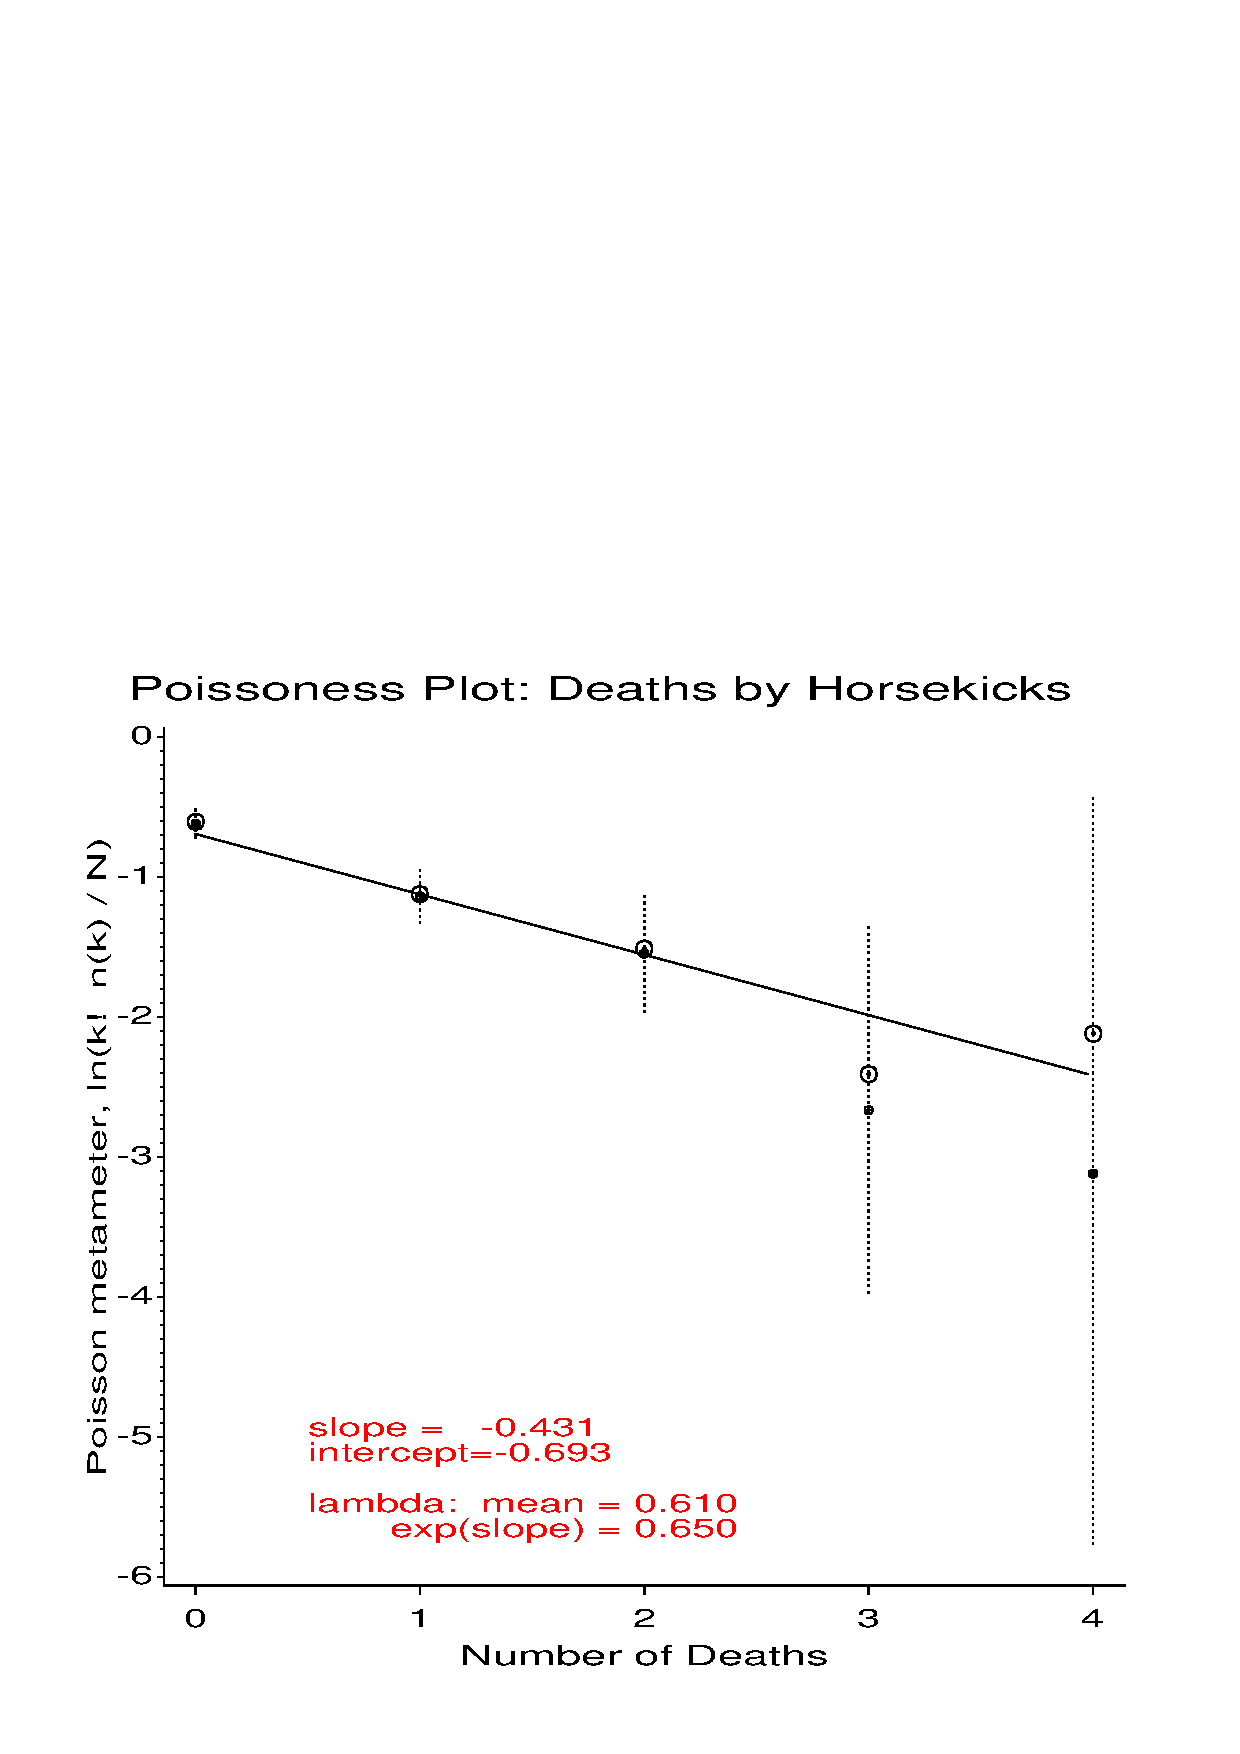
\includegraphics[scale=.5]{poisdemo1}\graphicsfile{ch2/fig/poisdemo1.eps}{}
  \caption[Poissonness plots for the horse kick data]{Poissonness plots
for the horse kick data.  The data fits the Poisson distribution
reasonably well.}\label{fig:poisdemo1}
\end{figure}

The leveled Poissonness plot (see \figref{fig:poisdemo2}) is produced by the \texttt{\%POISPLOT} statement
below, specifying \pname{LAMBDA=.610}.
%% input: /users/faculty/friendly/sasuser/catdata/poisdemo.sas
%% last modified: 08-Apr-99 12:38
\begin{listing}
title;
%poisplot(data=horskick, count=Deaths, freq=corpsyrs,
          lambda=.610, plot=dist);
run;
\end{listing}

\begin{figure}[htb]
  \centering
  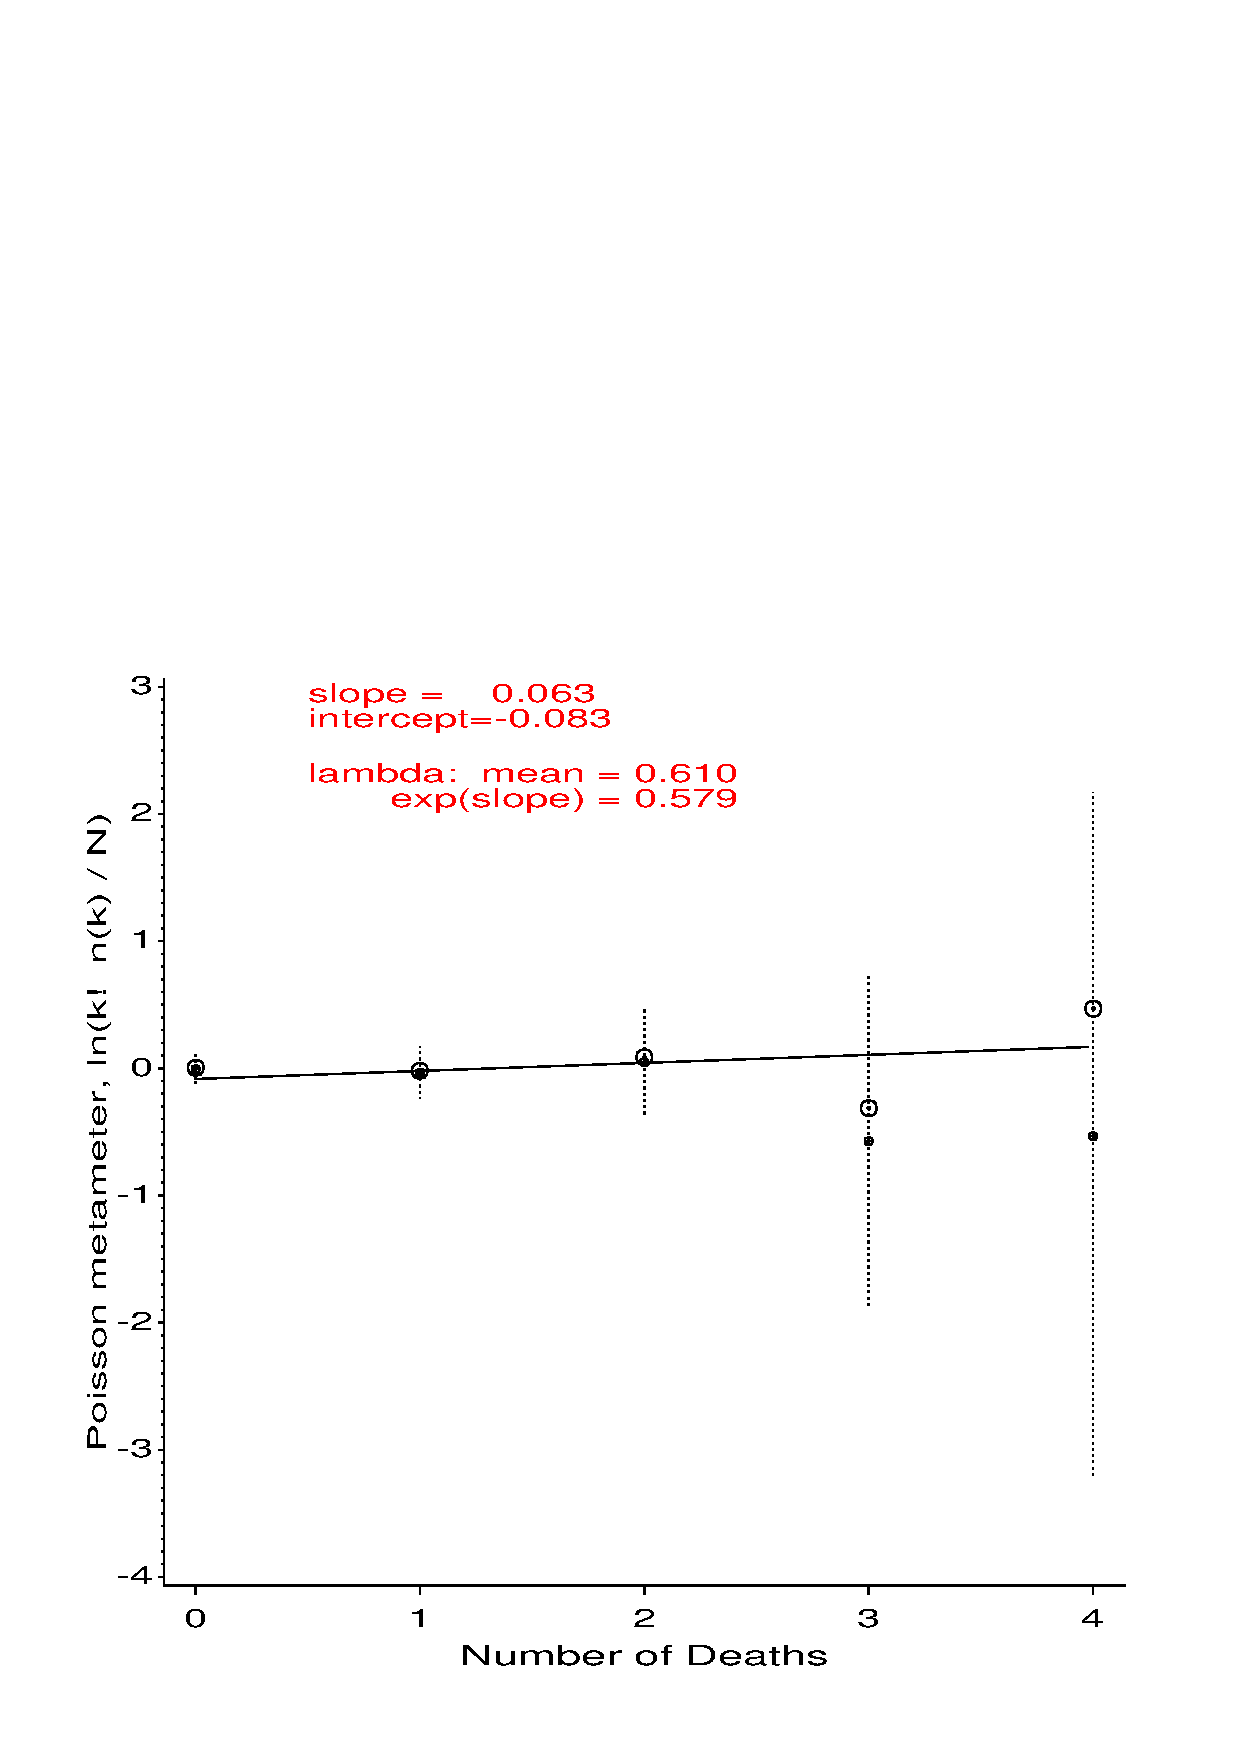
\includegraphics[scale=.5]{poisdemo2}\graphicsfile{ch2/fig/poisdemo2.eps}{}
  \caption[Leveled poissonness plot for the horse kick data]{Leveled poissonness plot for the horse kick data.}\label{fig:poisdemo2}
\end{figure}
In both plots the fitted line is within the confidence intervals;
the widths of the intervals for $k > 2$ are graphic reminders that these observations
have relatively low precision.

For comparison, \figref{fig:poismad1} shows the Poissonness plot
for the occurrences of \emph{may} in the
Federalist Papers (\tabref{tab:madison}).
The systematic curvature in the plot, judged relative to the confidence
intervals,
 indicates that these data do not follow a Poisson distribution.
\end{Example}

\begin{figure}[htb]
  \centering
  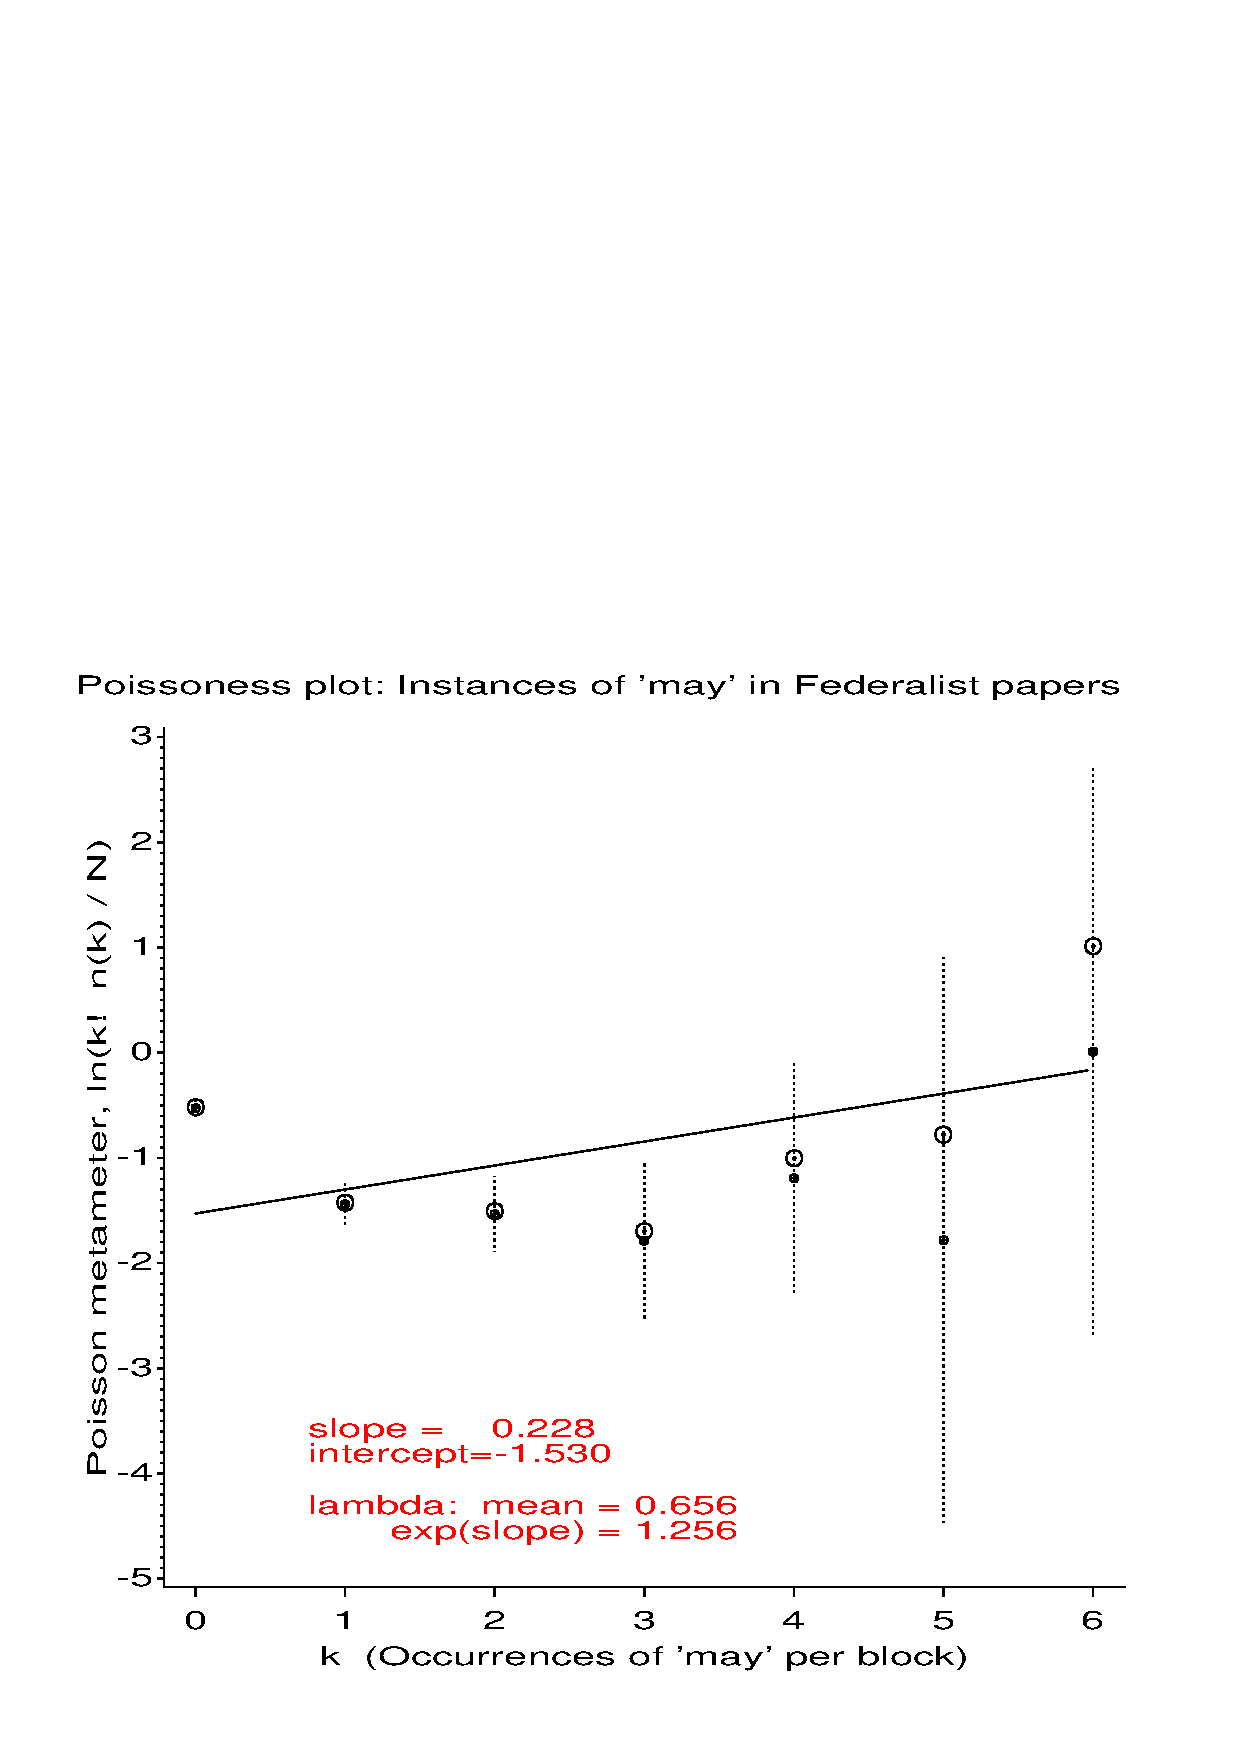
\includegraphics[scale=.5]{poismad1}\graphicsfile{ch2/fig/poismad1.eps}{}
  \caption[Poissonness plot for the Federalist Papers data]{Poissonness plot for the Federalist Papers data.
The systematic curvature in the plot indicates that this data does not follow a Poisson distribution.}\label{fig:poismad1}

\end{figure}
\subsection{Leverage and influence}
In standard models for quantitative data, common diagnostic techniques
attempt to estimate the effect that each observation has upon the
parameter estimates.
For linear models, these include measures of
\glossterm{leverage}---the potential
that an observation has to influence our results (due to its location
on the predictors),
and \glossterm{influence}---the actual effect this observation has
on parameter estimates and fitted values.

For discrete distributions, \citet{HoaglinTukey:85} derive
measures which are similar in spirit,  though based on the change in
the estimate of $ \lambda$ at each value of $k$ which would be
required to make the observed count metameter $\phi(n_k^{*})$
equal to its fitted value,
$\phi(m_k(\lambda_0))$ calculated using a contemplated or estimated $ \lambda_0$.

For the Poisson distribution, their analysis leads to the relation
\begin{equation}\label{eq:levpois}
\log \frac{\phi(n_k^{*})}{\phi(m_k(\lambda_0))}
= ( \lambda - \lambda_0 ) \left( \frac{k}{\lambda_0} - 1 \right)
\period
\end{equation}
Equation \eqref{eq:levpois} is 
a line through the origin with slope equal to $( \lambda - \lambda_0 )$.
By analogy with least squares regression through the origin
(where leverage is proportional to $x$), Hoaglin and Tukey
refer to $(k/\lambda_0) - 1$ as the leverage of point $k$.

Their parameter change plot shows each observation in the discrete
distribution as a point with vertical coordinate proportional to
$ \log [ \phi(n_k^{*}) / \phi(m_k(\lambda_0)) ] =
  \log ( \phi(n_k^{*})) - \log \phi(m_k(\lambda_0))$
and horizontal coordinate proportional to $k/\lambda_0 - 1$.
In this plot (see \figref{fig:poisdemo3}), the slope of
a line from the origin to a point shows the change in the Poisson
parameter, $\lambda - \lambda_0$ indicated by that
point.
The horizontal coordinate is proportional to the potential
of that observation to affect the Poisson parameter $\lambda$.

An alternative version of this plot, more in the spirit of the
influence plots for \loglin{} models and logistic regression
to be described later in this book, plots the
parameter change, $\lambda - \lambda_0$ directly on the
vertical axis against the same horizontal leverage value,
and uses a bubble whose size represents influence
as the plotting symbol.
%[More to be added here]

The parameter change plot and the influence plot are produced
with the \macro{POISPLOT} by including the keyword
\texttt{INFL} in the \texttt{PLOT=} parameter (i.e., \texttt{PLOT=DIST INFL}
gives all plots).
For the horse kick data, these plots are shown in
\figref{fig:poisdemo3} and \figref{fig:poisdemo4}.

\begin{figure}[htb]
  \centering
  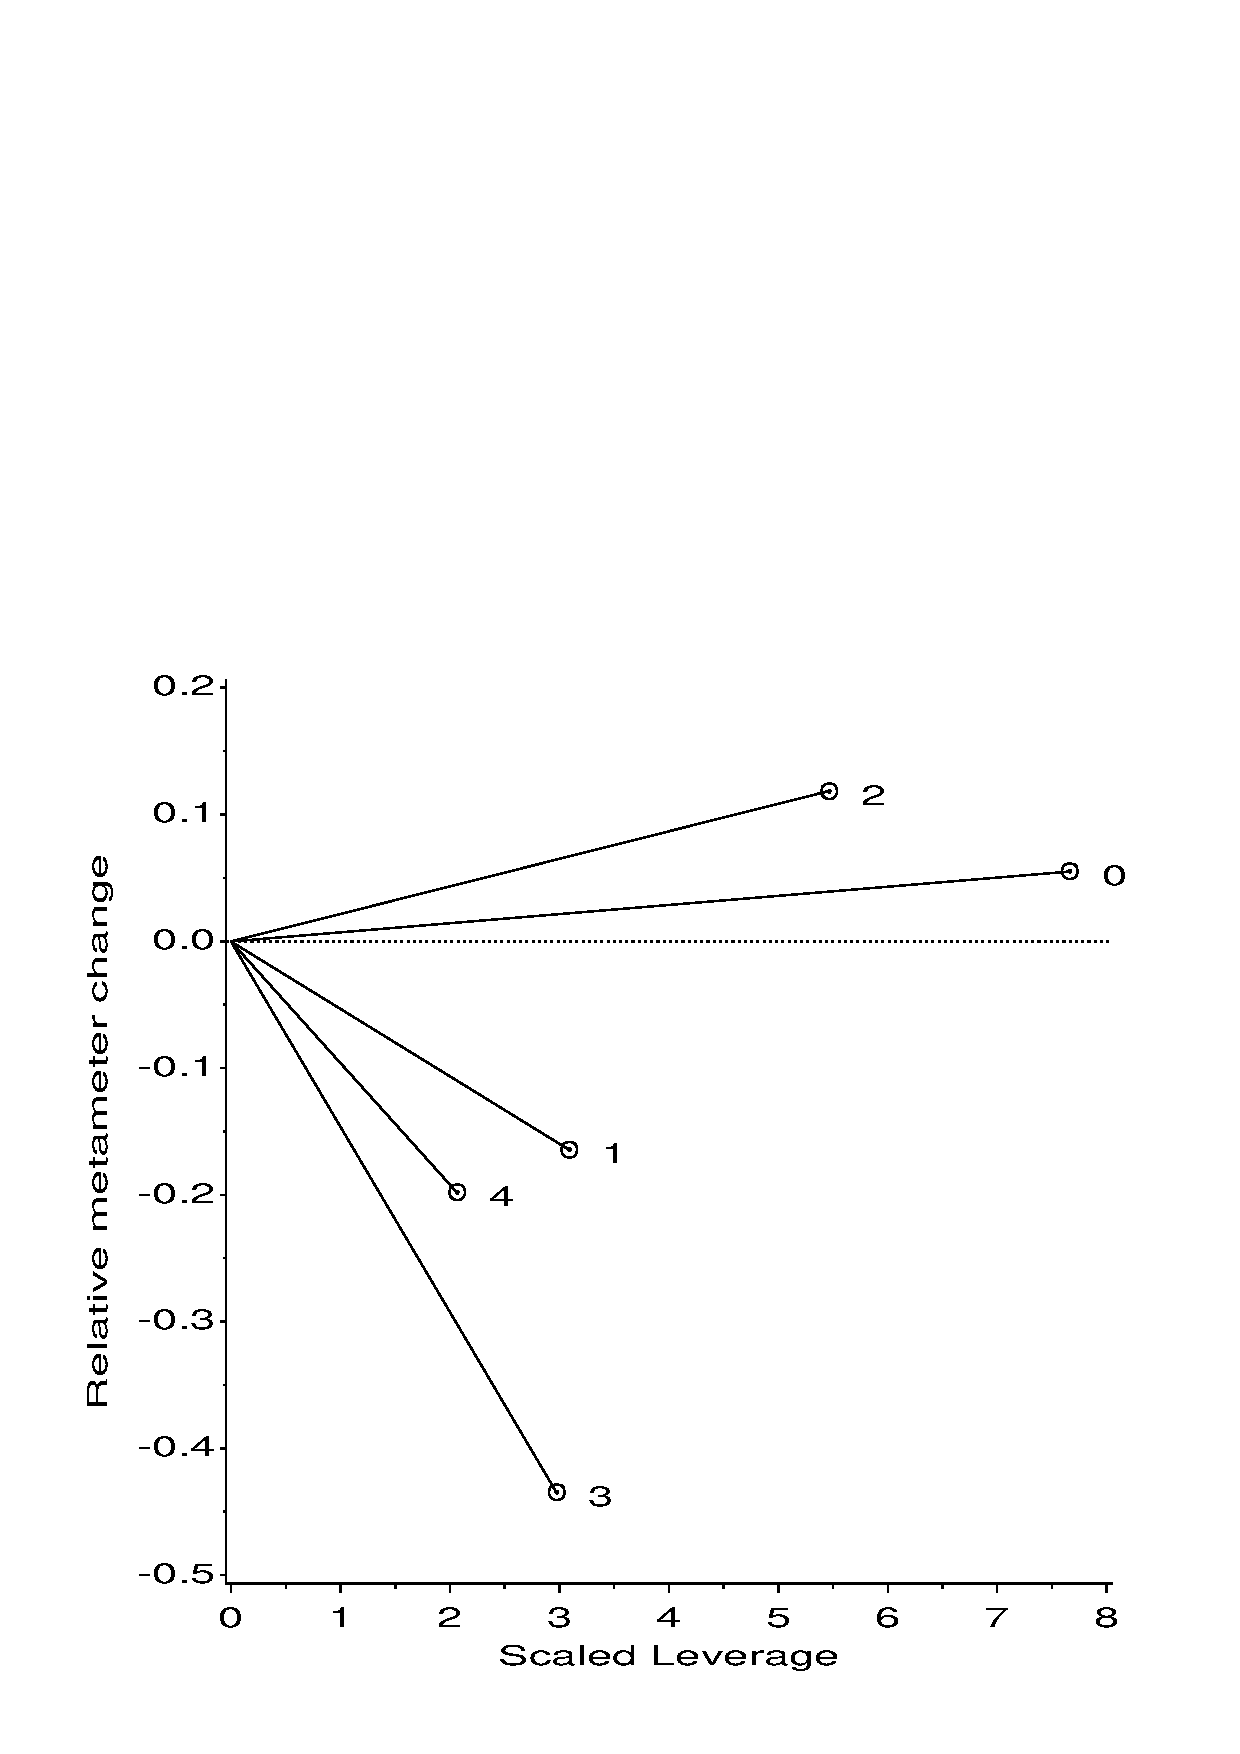
\includegraphics[scale=.5]{poisdemo3}\graphicsfile{ch2/fig/poisdemo3.eps}{}
  \caption[Parameter change plot for the Poisson parameter]{Parameter change
plot for the Poisson parameter, fitting the horse kick data.
The horizontal coordinate of each point is proportional to the potential of that observation to affect the value of $\lambda$.
The slope of the line through the origin is proportional to the
change in the count metameter.}\label{fig:poisdemo3}
\end{figure}
In \figref{fig:poisdemo3} we see that
the point corresponding to $k=0$ has the greatest leverage, but
influences $\lambda$ very little.
The point for $k=3$ has only moderate leverage, but has the greatest
impact on the Poisson parameter.
In \figref{fig:poisdemo2}
we see that the circle symbol for $\phi(n_k^{*})$
at $k=3$ is furthest from the
line.
\figref{fig:poisdemo4} shows that this point indicates a $\lambda$
value about 0.15 smaller than the estimated value.
\begin{figure}[htb]
  \centering
  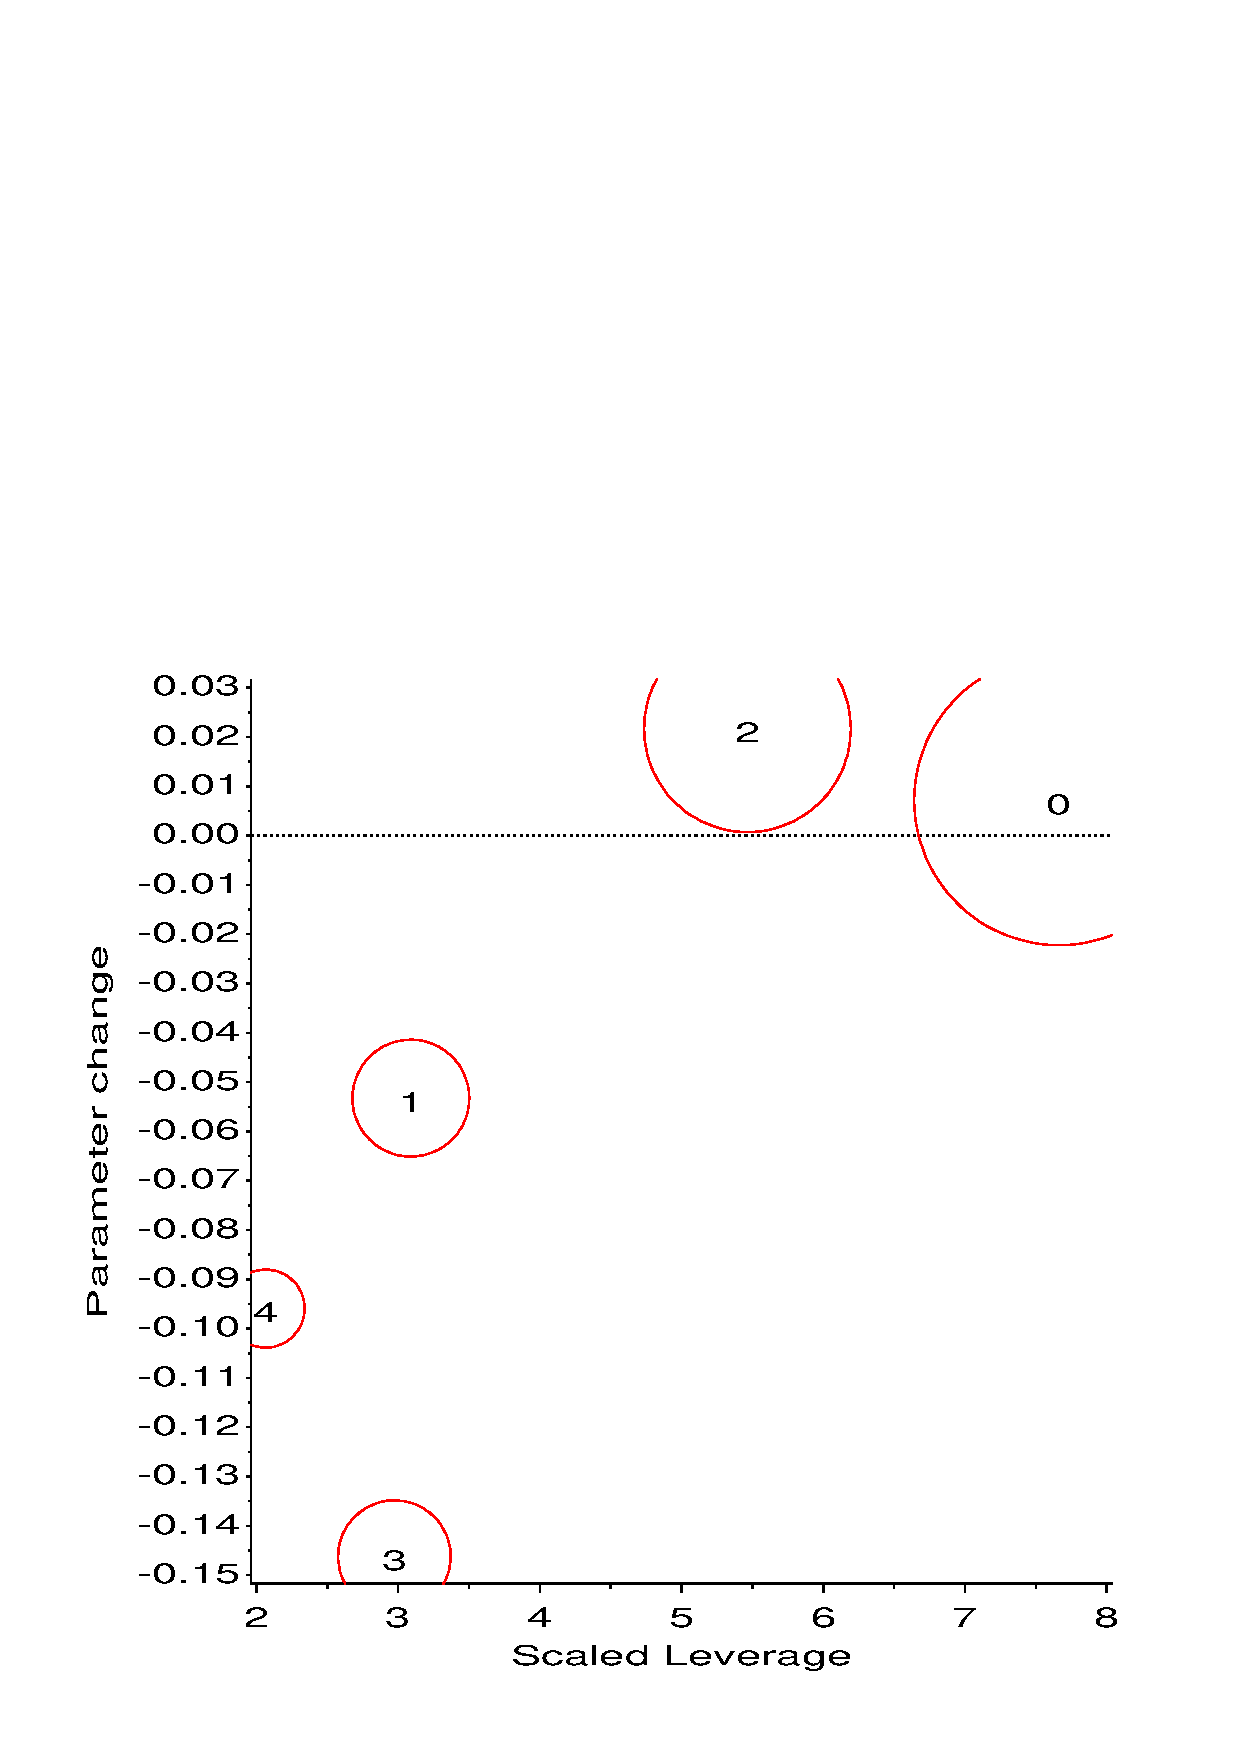
\includegraphics[scale=.5]{poisdemo4}\graphicsfile{ch2/fig/poisdemo4.eps}{}
  \caption[Influence plot for the Poisson parameter]{Influence plot
for the Poisson parameter, fitting the horse kick data.
  The ordinate shows the indicated change in $\lambda$
directly, and the bubble size is proportional to
influence.}\label{fig:poisdemo4} \end{figure}


\ix{Poissonness plot|)}

\subsection{Plots for other distributions}\label{sec:discrete-other}
As described in \secref{sec:pwrseries}, the binomial, Poisson, negative binomial,
geometric, and logseries distributions are all members of the
general  power series family of discrete distributions.
For this family, \citet{HoaglinTukey:85} develop similar plots
of a count metameter against $k$ which appear as a straight line
when a data distribution follows a given family member.

The distributions which can be analyzed in this way are shown in
\tabref{tab:distparms}, with the interpretation given to the
slope and intercept in each case.
For example, for the Binomial distribution, a ``binomialness''
plot is constructed by plotting $\log n_k^{*} / N \binom{n}{k}$
against $k$.  If the points in this plot approximate a straight
line, the slope is interpreted as $\log (p/(1-p))$, so the
binomial parameter $p$ may be estimated as $p = e^b/(1+e^b)$.
\begin{table}[htb]
\caption[Plot parameters for five discrete distributions]{Plot parameters for five discrete distributions. In each case the count metameter, $\phi
(n_k^{*})$ is plotted against $k$, yielding a straight line when the data
follow the given distribution.}
\label{tab:distparms}
 \begin{center}
\begin{tabular}{p{2.4cm}llll}
  \hline\\[.5ex]
  \tableheader
%              & Probability      & Count                      & Theoretical & Theoretical \\
%Distributiion & function, $p(k)$ & metameter, $\phi(n_k^{*})$ & Slope ($b$) & Intercept ($a$)\\[1ex]
  \multilineL{Distribution\\} & \multilineL{Probability\\function, $p(k)$} & \multilineL{Count)\\metameter, $\phi(n_k^{*})$} & \multilineL{Theoretical\\ slope ($b$)} &
  \multilineL{Theoretical\\ intercept ($a$)}
  \hline \\[.5ex]
Poisson          & $e^{-\lambda }\lambda ^k/k!$ & $\log (k!n_k^{*}/N)$ & $\log
(\lambda )$ & -$\lambda $ \\[.7ex]
%
Binomial          & $\binom nkp^k(1-p)^{n-k}$ & $\log \left( n_k^{*}/N\binom
nk\right) $ & $\log \left(\frac{p}{1-p}\right)$ & $n\log (1-p)$ \\[.7ex]
%
Negative binomial & $\binom{n+k-1}kp^n(1-p)^k$ & $\log \left( n_k^{*}/N%
\binom{n+k-1}k\right) $ & $\log (1-p)$ & $n\log (p)$ \\[.7ex]
%
Geometric         & $p(1-p)^k$ & $\log \left( n_k^{*}/N\right) $ & $\log (1-p)$ & $\log (p)$ \\[.7ex]
%
Log series        & $\theta ^k/[-k\log (1-\theta )]$ & $\log \left(
kn_k^{*}/N\right) $ & $\log (\theta )$ & $-\log \left( -\log (1-\theta)\right) $ \\[1ex]%
  \hline
  \multicolumn{5}{p{\textwidth}}{\emph{Source}: adapted from \citet{HoaglinTukey:85}, Table 9-15.} \\
\end{tabular}
 \end{center}
\end{table}



Unlike the Ord plot, a different plot is required for each distribution,
because the count metameter, \(\phi ( n_k )\), differs
from distribution to distribution.
Moreover, systematic deviation from a linear relationship does not
       indicate which distribution provides a better fit.
However, the attention to robustness, and the availability of confidence
intervals and influence diagnostics make this a highly useful tool
for visualizing discrete distributions.


\subsubsection{\macro{DISTPLOT}}
The \macro{DISTPLOT} (see \macref{mac:distplot}) carries out the analysis and produces overall
distribution plots and influence plots for the members of the
power series distributions shown in \tabref{tab:distparms}.
As with the \macro{GOODFIT} values for parameters for a given distribution
may be supplied
in the \mparm{PARM}{DISTPLOT}.

When the value of the distribution parameter
is not supplied, the macro produces the overall distribution plot
whose slope $b$ (and intercept $a$) are used to find graphical
estimates of the parameter.
For most distributions, the available MLE or moments estimates
given in \secref{sec:discrete-distrib}
are also calculated and displayed in the plot.
When the value of the distribution parameter is supplied,
a leveled plot is produced, with graphical parameter estimates adjusted
for the leveling.

\begin{Example}[saxony3]{Families in Saxony}
Our analysis in \exref{ex:saxony1} and \exref{ex:saxony2} of
the Saxony data
showed that the distribution of male children had slightly heavier tails
than the binomial.
We can see this even more clearly in the distribution diagnostic
plot produced
by the \macro{DISTPLOT}.  For a binomial distribution, we might call
this a ``binomialness plot''.

\figref{fig:saxony1} is produced with the statement
\begin{listing}
%distplot(data=saxony, count=males, freq=families, dist=binomial);
\end{listing}
The systematic curvature of the points again indicates the inadequacy
of the binomial, and the widths of the intervals around the points
show that the two extreme points are of limited reliability.
Comparing this plot with the hanging rootogram (\figref{fig:saxony}),
we see that heavy-tailed distributions will tend to curve upwards.
We also see that the estimate of $p = \exp(b) / [1+\exp(b)] $ from the slope of the fitted
line is quite close to the maximum likelihood estimate.
\begin{figure}[htb]
  \centering
  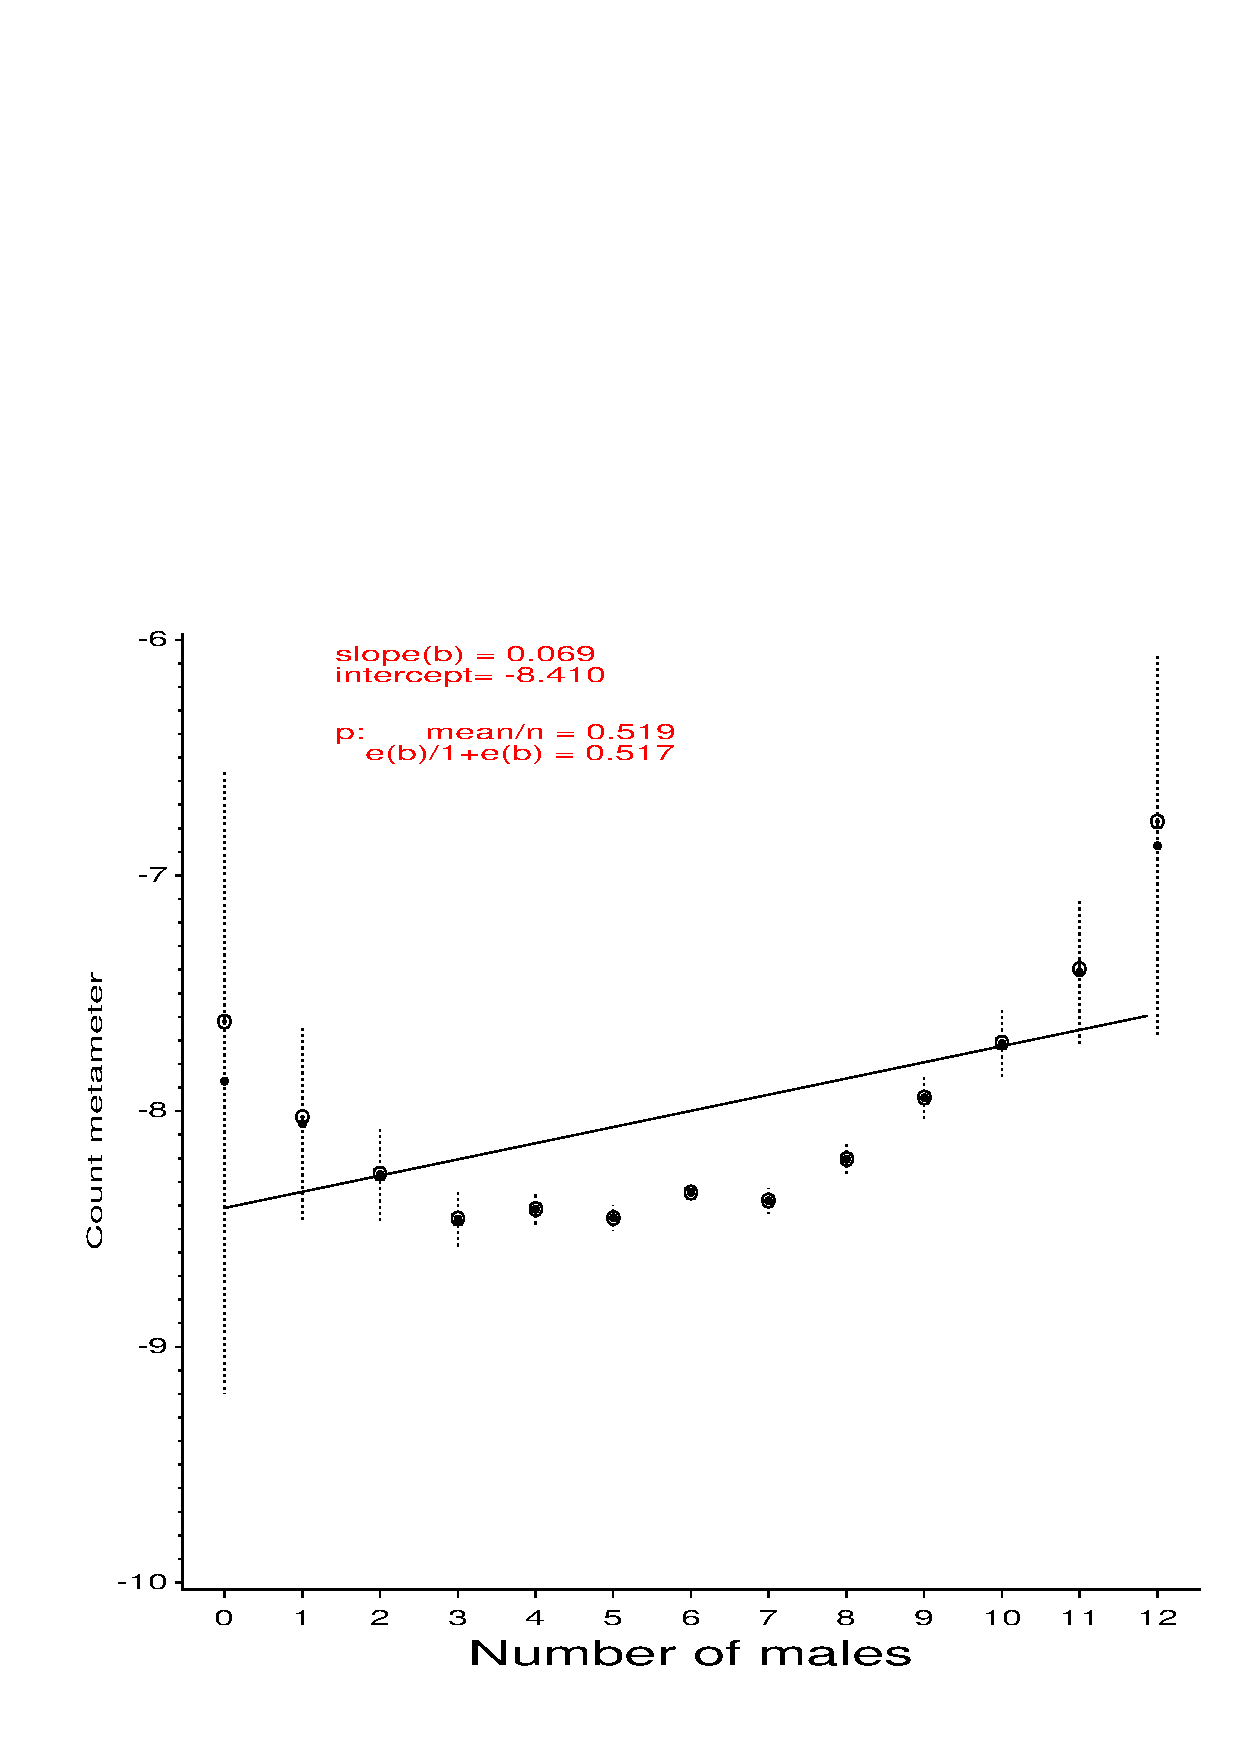
\includegraphics[scale=.6]{saxony1}\graphicsfile{ch2/fig/saxony1.eps}{}
  \caption{Binomialness plot for the distribution of males in Saxony families. }%
  \label{fig:saxony1}
\end{figure}
\end{Example}

%\section{Chapter summary}
\begin{itemize}
\item Correspondence analysis is an exploratory technique, designed to
show the row and column categories in a two- (or three-) dimensional
space.  These graphical displays, and various extensions, provide
ways to interpret the patterns of association and visually explore 
the adequacy of certain \loglin models.

\item The scores assigned to the categories of each variable are optimal
in several equivalent ways.
Among other properties,
they maximize the (canonical) correlations between the quantified
variables (weighted by cell frequencies), and make the regressions
of each variable on the other most nearly linear, for each CA dimension.

\item Multi-way tables may be analyzed in several ways.
In the ``stacking'' approach, two or more variables may be combined
interactively in the rows and/or columns of an \nway table.
Simple CA of the restructured table reveals associations between
the row and column categories of the restructured table,
but hides associations between the variables combined interactively.
Each way of stacking corresponds to a particular \loglin model
for the full table.

\item Multiple \ca is a generalization of CA to two or more variables
based on representing the data as an indicator matrix, or the Burt matrix.
The usual MCA provides an analysis of the joint, bivariate relations
between all pairs of variables.

% \item An extended form of MCA provides a means to display higher-order
% associations among multiple categorical variables.
% For $2^Q$ tables composed of $Q$ binary variables, this analysis yields
% simple geometric relations that may be interpreted in terms of odds ratios.
% \TODO{Delete this if \secref{sec:ca-mcainter} is not included.}

\item The biplot is a related technique for visualizing the elements of
a data array by points or vectors in a joint display of their row and
column categories. A standard CA biplot represents the contributions to
lack of independence as the projection of the points for rows
(or columns) on vectors for the other categories.

\item Another application of the biplot to \ctab data is described, based on analysis
of log frequency.
This analysis also serves to diagnose patterns of independence and
partial independence in two-way and larger tables.
\end{itemize}

%\section{Further reading}


\bibliographystyle{plain}
\bibliography{bibtex_example}

\printindex

\end{document}
